\section{EXTRACTING THE \texorpdfstring{$x$}{x}-DEPENDENCE}

\subsection{ Constraint $b\cdot P \neq 0$ for ($P_1=-1$)}
From
\begin{align}
    \frac{v \tcdot b}{v \tcdot P} = b \tcdot P \frac{R(\zetahat^2)}{\mN^2}
\end{align}
We have,
\begin{align}
    b_{1}|v|\left[\frac{P_{1}}{m_{N}}\left(\hat{\zeta}-\sqrt{\hat{\zeta}^2+1}\right)+\hat{\zeta}\frac{m_{N}}{P_{1}}\right]=\vec{v}_{T}\cdot\vec{b}_{T}
\end{align}
let $\vec{v}_{T}=(0,v_{3})$ and $\vec{b}_{T}=(b_{2},0)$
\begin{align}
    \mN &= 1067\text{ MeV};~~~~P_{1}=-\frac{2\pi}{L}=-\frac{2\pi}{32\times 0.114\text{ fm}}=-339.3\text{ MeV},
\end{align}
then
\begin{align}
   \Longrightarrow \left[\frac{P_{1}}{m_{N}}\left(\hat{\zeta}-\sqrt{\hat{\zeta}^2+1}\right)+\hat{\zeta}\frac{m_{N}}{P_{1}}\right]&=0\\
    \Longrightarrow \hat{\zeta} &=\sqrt{\frac{P_{1}^2}{m_{N}^{2}\left(\frac{m_{N}^{2}}{P_{1}^{2}}+2\right)}}\\
    \Aboxed{\hat{\zeta} &= \pm 0.0922238}.
\end{align}
Now,
\begin{align}
    \hat{\zeta}&=\frac{-v_{1}P_{1}}{|v|\mN}=\frac{-v_{1}P_{1}}{\left(\sqrt{v_{1}^{2}+0^{2}+v_{3}^{2}}\right)m_{N}}
\end{align}
on solving for $v_{1}$,
\begin{align}
    \Longrightarrow\Aboxed{v_{1}=\pm 0.303023~v_{3}}
\end{align}
Similarly, we find for all momenta as follows
\begin{table}[h!]
    \centering
    \begin{tabular}{|c|c|c|}
    \hline
        $\vect{P}\cdot a\hat{L}/(2\pi)$ & $\hat{\zeta}$ &  $v_{1}$\\
        \hline
        $(-1,0,0)$ & $\pm 0.090772$ &$v_{1}=\pm 0.301~v_{3}$\\
        \hline
        $(-2,0,0)$ & $\pm 0.294367$ &$v_{1}=\pm 0.531~v_{3}$\\
        \hline
        $(-3,0,0)$ & $\pm 0.539684$ &$v_{1}=\pm 0.689~v_{3}$\\
        \hline
        $(-4,0,0)$ & $\pm 0.785756$ &$v_{1}=\pm 0.786~v_{3}$\\
        \hline
    \end{tabular}
    \caption{Directions of $\vect{v}$ vector}
    \label{tab:placeholder}
\end{table}

So, we have
\begin{table}[h!]
    \centering
    \begin{tabular}{|c|c|c|}
    \hline
       $\vect{\bvec}/a$  &  $\eta \vect{v}/a$ & $\vect{P}\cdot a\hat{L}/(2\pi)$\\
       \hline
        $(b_{1},b_{2},0)$ & $ \eta\cdot(v_{1},0,v_{3})$, $\eta=0,\cdots,10$  & $(n,0,0)$, $n=-1,-2,-3,-4$\\
        \hline
    \end{tabular}
    \caption{Parameters of Lattice QCD calculations}
    \label{tab:my_label}
\end{table}

\begin{figure}
    \centering
    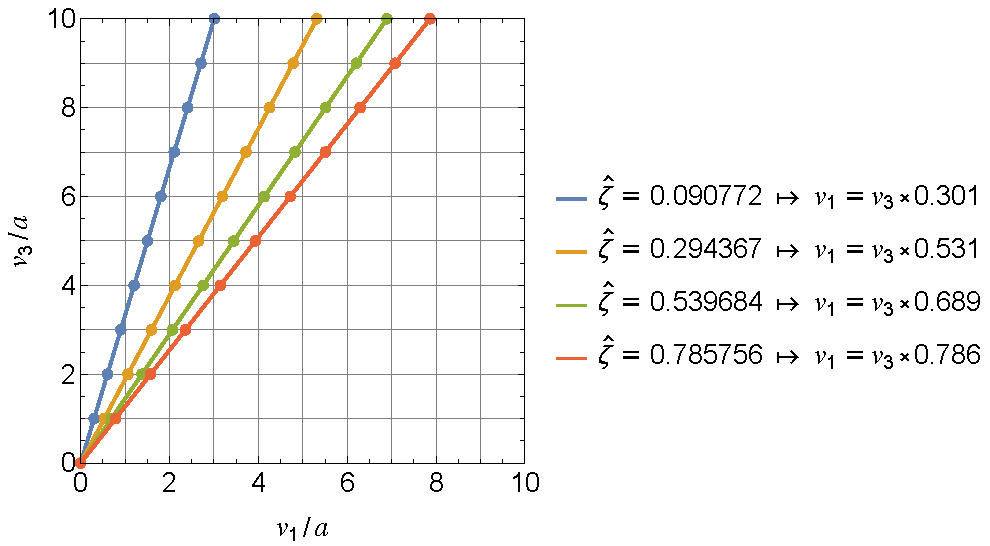
\includegraphics[width=0.5\linewidth]{plots/kinematics_interpolation/v1_v2_allzetahat_plot.pdf}
    \caption{Caption}
    \label{fig:placeholder}
\end{figure}

\pagebreak
\subsubsection{Off-axis \texorpdfstring{$\vect{v}$}{TEXT}}
\begin{figure}[h!]
    \centering
    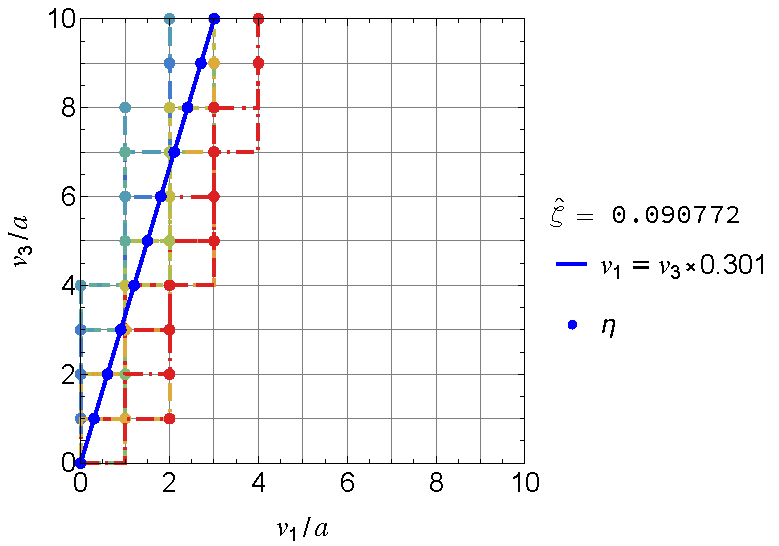
\includegraphics[width=0.5\linewidth]{plots/kinematics_interpolation/v1_v2_withPath_forP-1_plot.pdf}
    \caption{Caption}
    \label{fig:placeholder}
\end{figure}
\begin{figure}[h!]
    \centering
    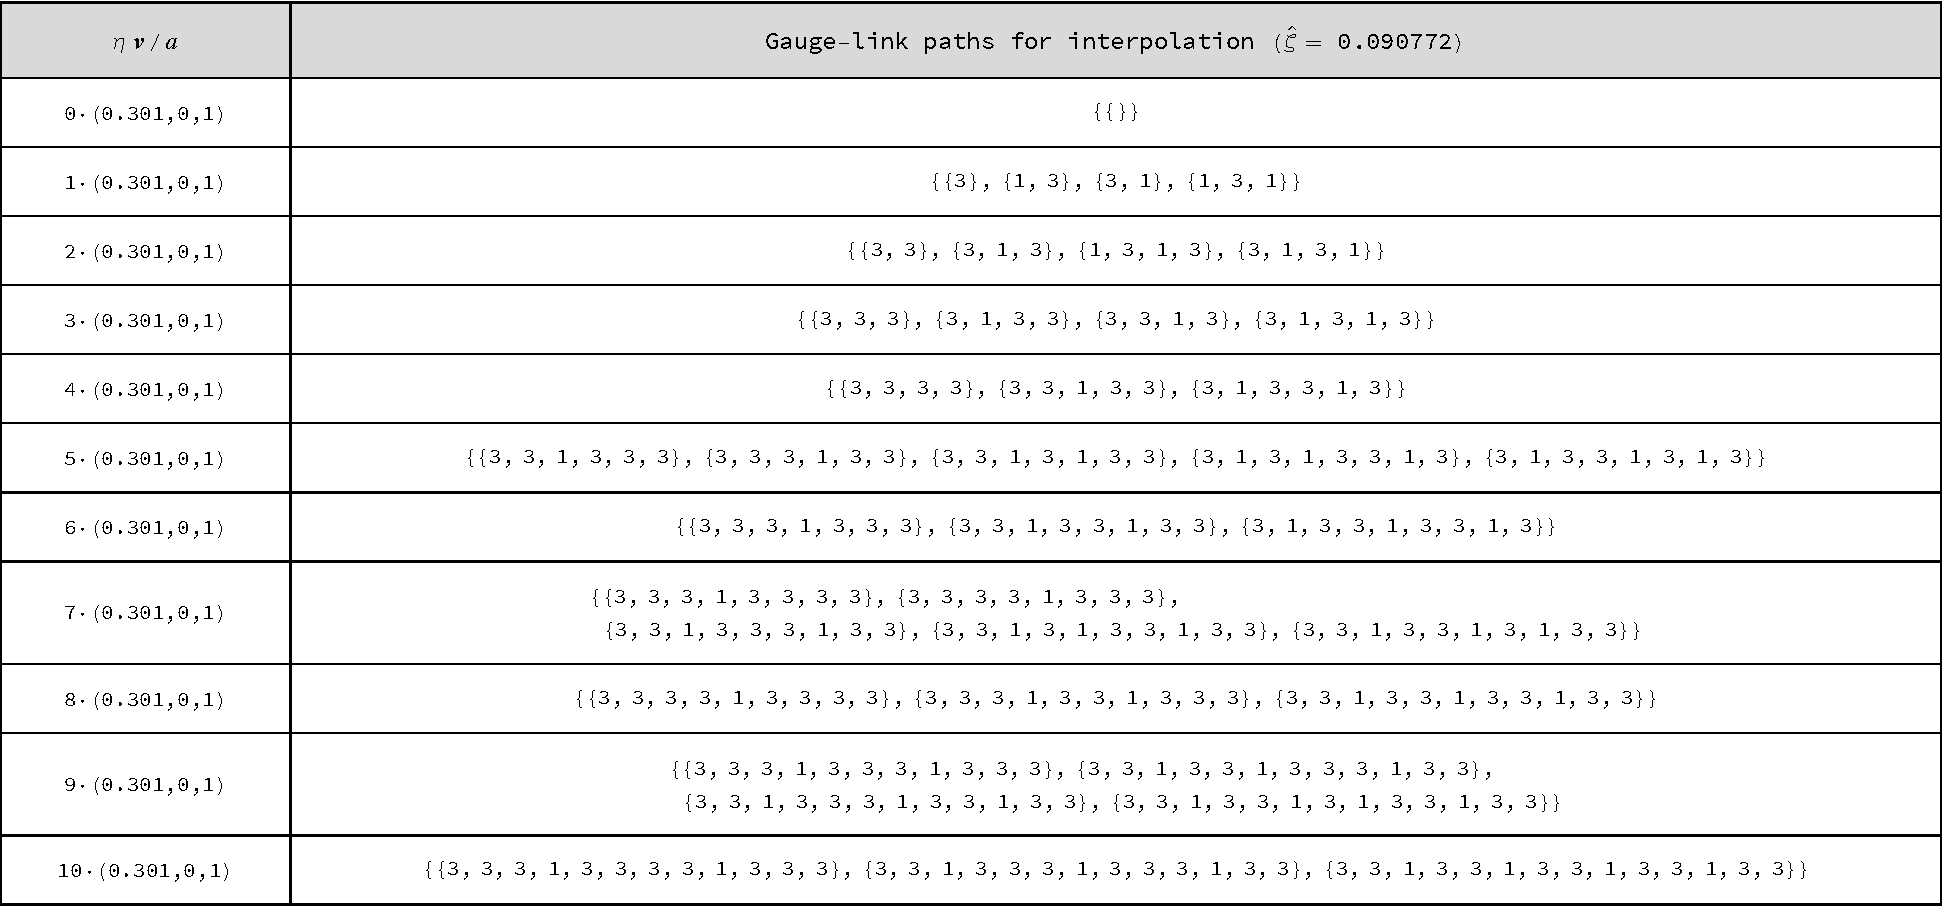
\includegraphics[width=0.8\linewidth]{plots/kinematics_interpolation/eta_gauge_links_forP-1_table.pdf}
    \caption{Caption}
    \label{fig:placeholder}
\end{figure}

\begin{figure}[h!]
    \centering
    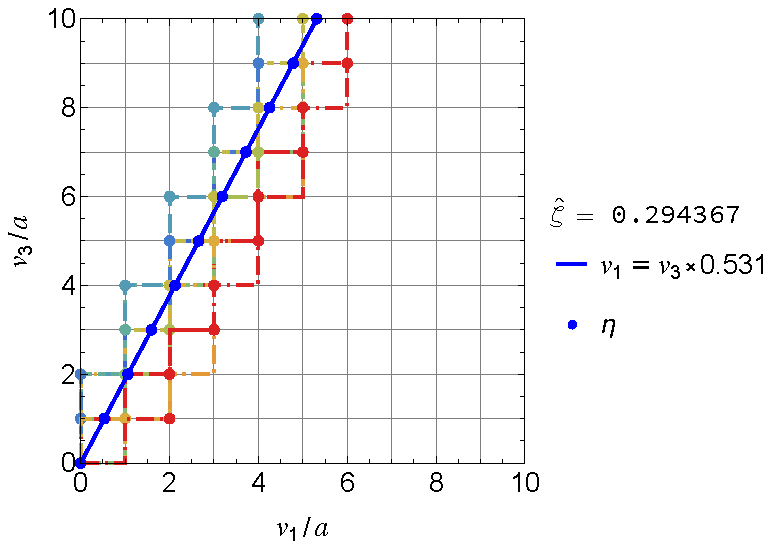
\includegraphics[width=0.5\linewidth]{plots/kinematics_interpolation/v1_v2_withPath_forP-2_plot.pdf}
    \caption{Caption}
    \label{fig:placeholder}
\end{figure}
\begin{figure}[h!]
    \centering
    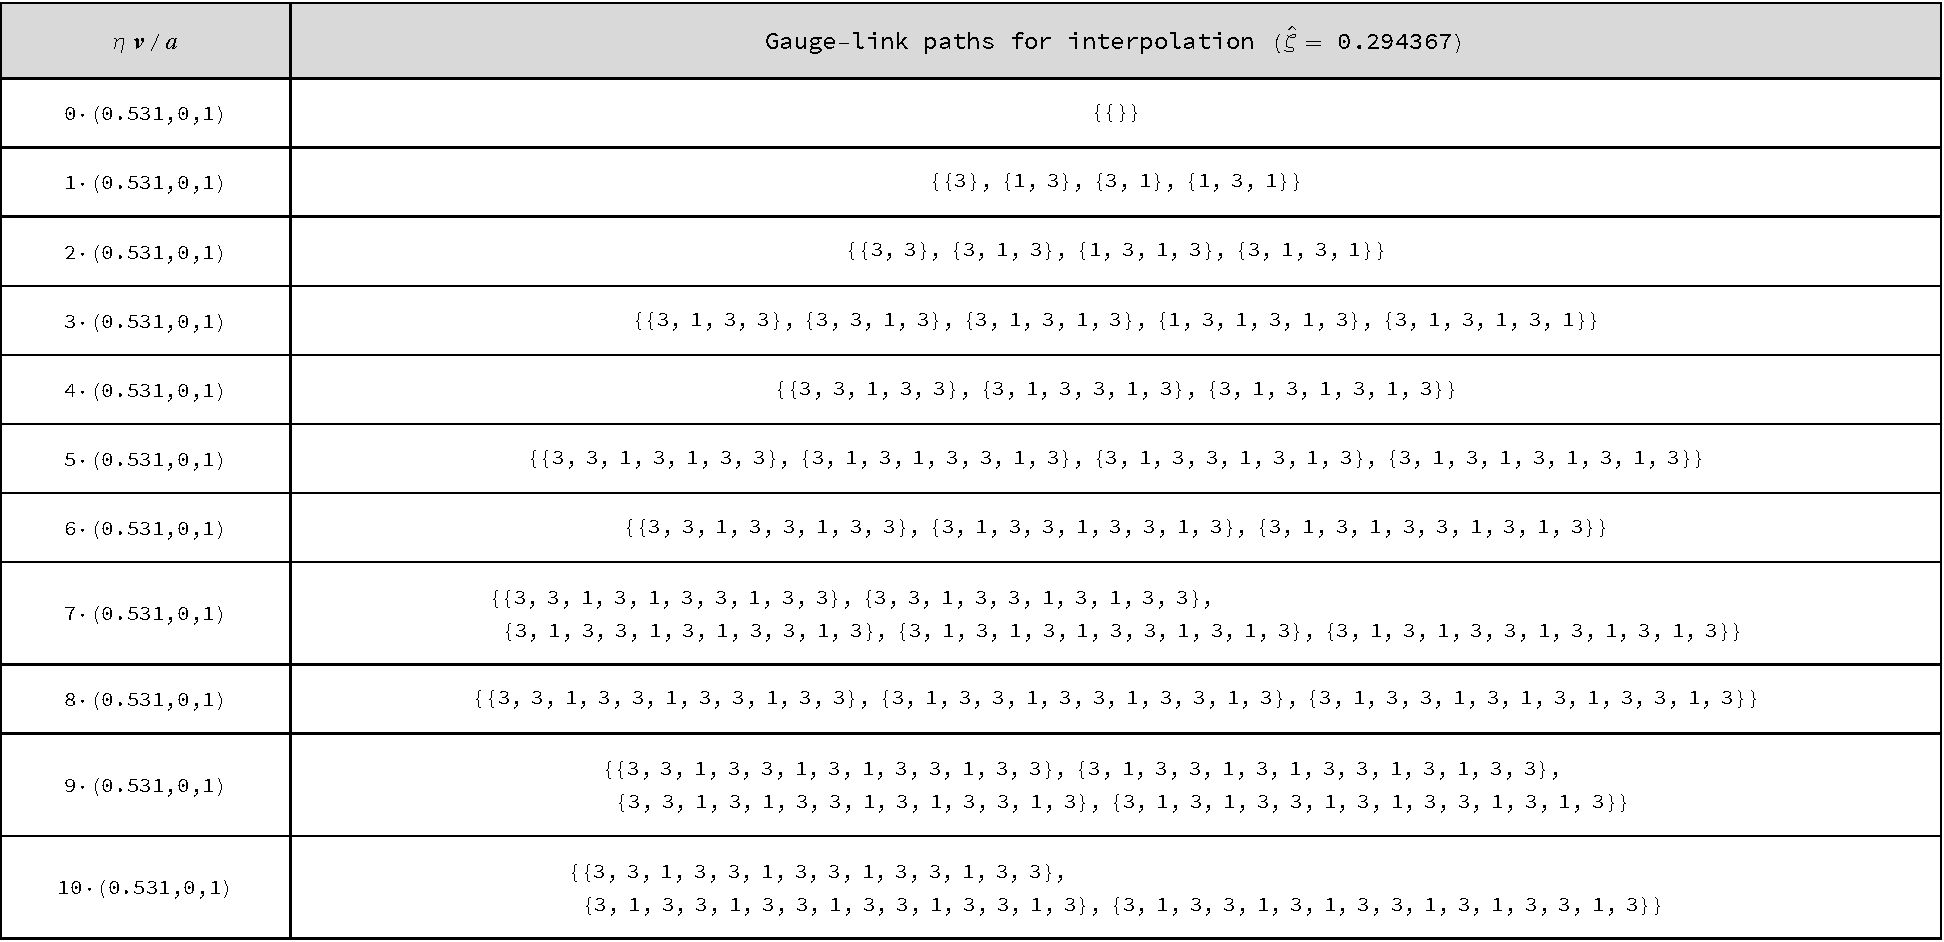
\includegraphics[width=0.8\linewidth]{plots/kinematics_interpolation/eta_gauge_links_forP-2_table.pdf}
    \caption{Caption}
    \label{fig:placeholder}
\end{figure}

\begin{figure}[h!]
    \centering
    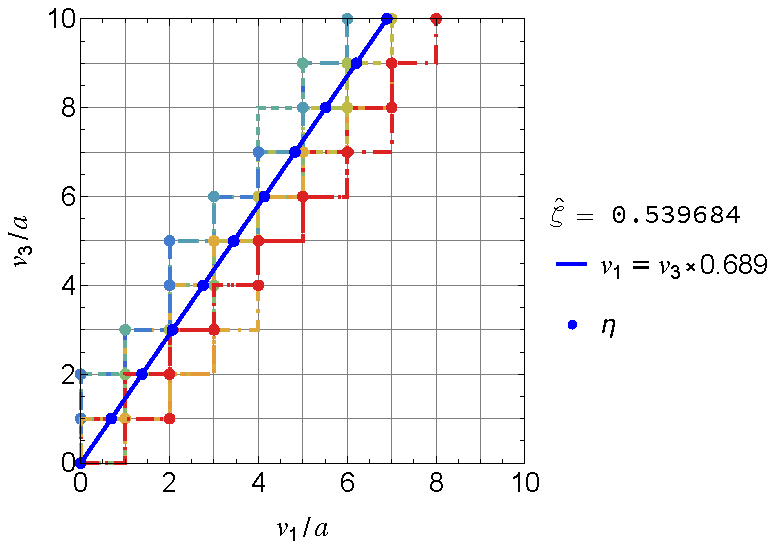
\includegraphics[width=0.5\linewidth]{plots/kinematics_interpolation/v1_v2_withPath_forP-3_plot.pdf}
    \caption{Caption}
    \label{fig:placeholder}
\end{figure}
\begin{figure}[h!]
    \centering
    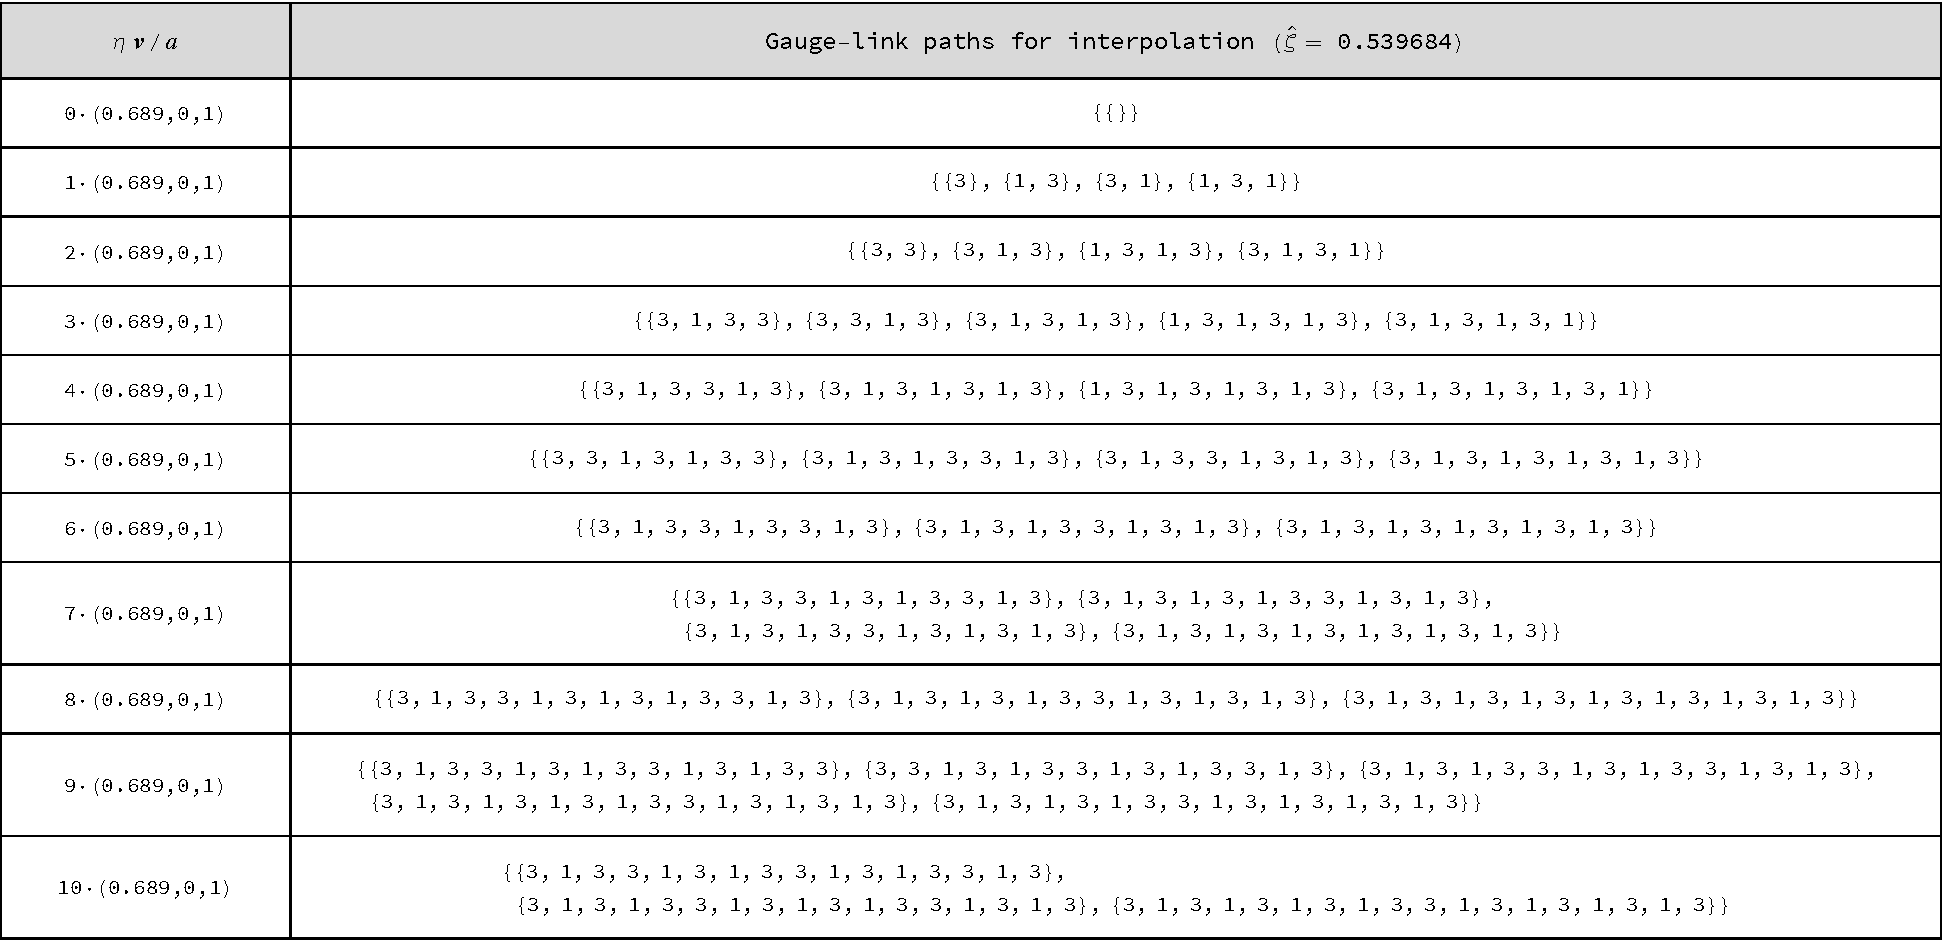
\includegraphics[width=0.8\linewidth]{plots/kinematics_interpolation/eta_gauge_links_forP-3_table.pdf}
    \caption{Caption}
    \label{fig:placeholder}
\end{figure}

\begin{figure}[h!]
    \centering
    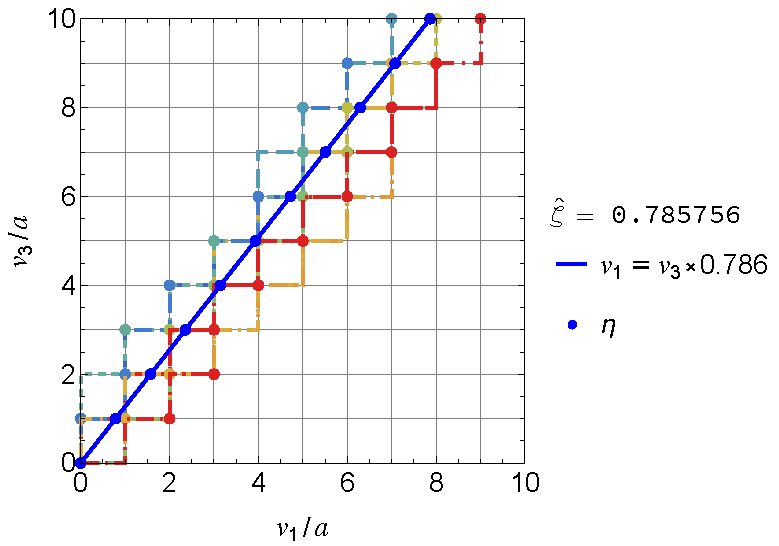
\includegraphics[width=0.5\linewidth]{plots/kinematics_interpolation/v1_v2_withPath_forP-4_plot.pdf}
    \caption{Caption}
    \label{fig:placeholder}
\end{figure}
\begin{figure}[h!]
    \centering
    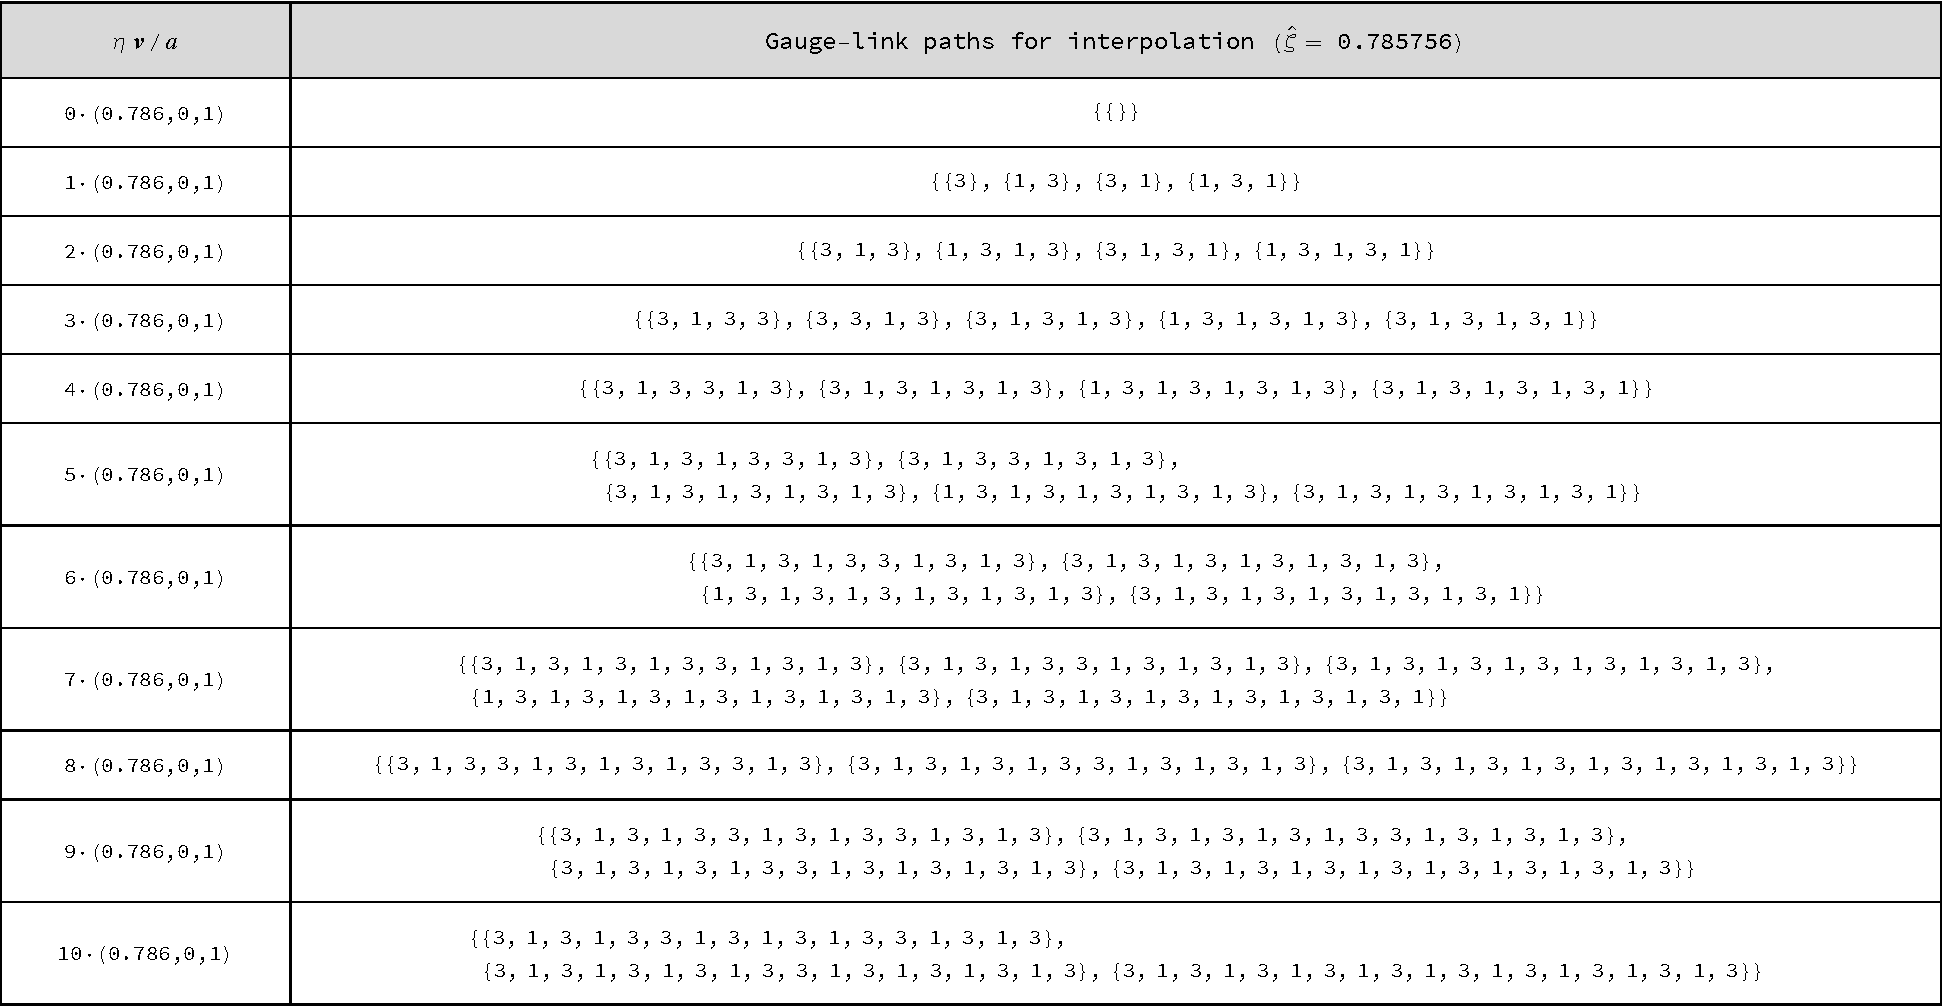
\includegraphics[width=0.8\linewidth]{plots/kinematics_interpolation/eta_gauge_links_forP-4_table.pdf}
    \caption{Caption}
    \label{fig:placeholder}
\end{figure}

\subsection{Deriving \texorpdfstring{$\widetilde \Phi^{[\gamma^+]}$}{TEXT}}
Let's start with the parametrization of the correlator \cite{BMush_Engelhardt2012},
\begin{align}
    \frac{1}{2}\widetilde \Phi^{[\gamma^\mu]}_{\unsub} & = 
		P^\mu\, \tAmp_2 - i \mN^2 \bvec^\mu\, \tAmp_3
		- i \mN \epsilon^{\mu \nu \alpha \beta} P_\nu \bvec_\alpha S_\beta\, \tAmp_{12} \nonumber \\ &
		~~+ \frac{\mN^2}{(v \tcdot P)} v^\mu\, \tBmp_1 
		+ \frac{\mN}{v \tcdot P} \epsilon^{\mu \nu \alpha \beta} P_\nu v_\alpha S_\beta\, \tBmp_7  
		- \frac{ i \mN^3}{v \tcdot P} \epsilon^{\mu \nu \alpha \beta} \bvec_\nu v_\alpha S_\beta\, \tBmp_8 \nonumber \\ &
		~~- \frac{\mN^3}{v \tcdot P} (\bvec \tcdot S) \epsilon^{\mu \nu \alpha \beta} P_\nu \bvec_\alpha v_\beta\, \tBmp_9
		- \frac{i \mN^3}{(v \tcdot P)^2} (v \tcdot S) \epsilon^{\mu \nu \alpha \beta} P_\nu \bvec_\alpha v_\beta \tBmp_{10}
\end{align}
 For the lattice calculations, it is, however, advantageous to start with an equivalent parametrization in which the structures explicitly depend on the staple extent $\eta$ and which is still well-defined for $ v\cdot P = 0$. Such a parametrization can be obtained from the parametrization above by replacing $v \rightarrow \eta v$ and by leaving out the factors $(v \tcdot P)^{-n}$. 
 \begin{align}
    \frac{1}{2}\widetilde \Phi^{[\gamma^\mu]}_{\unsub}=\frac{1}{2} R_{\gamma^{\mu}} E_N & =  
		P^\mu\, \tilde a_2 - i \mN^2 \bvec^\mu\, \tilde a_3
		- i \mN \epsilon^{\mu \nu \alpha \beta} P_\nu \bvec_\alpha S_\beta\, \tilde a_{12} \nonumber \\ &
		~~+ \mN^2 \eta v^\mu\, \tilde b_1 
		+ \mN \epsilon^{\mu \nu \alpha \beta} P_\nu \eta v_\alpha S_\beta\, \tilde b_7  
		-  i \mN^3 \epsilon^{\mu \nu \alpha \beta} \bvec_\nu \eta v_\alpha S_\beta\, \tilde b_8 \nonumber \\ &
		~~- \mN^3 (\bvec \tcdot S) \epsilon^{\mu \nu \alpha \beta} P_\nu \bvec_\alpha \eta v_\beta\, \tilde b_9
		-i \mN^3 (v \tcdot S) \epsilon^{\mu \nu \alpha \beta} P_\nu \bvec_\alpha \eta^2 v_\beta \tilde b_{10}
\end{align}
For $P^{\mu}=(E_N, -|\vec{P}^1|,0,0)$, $b^{\mu}=(0,b_{1},b_{2},0)$, $v^{\mu}=\pm n^{\prime}(0,v_{1},0,v_{3})$, $S^{\mu}=(0,0,0,1)$,
\begin{align}
    \frac{1}{2}\widetilde \Phi^{[\gamma^{0}]}_{\unsub} & = 
		P^0\, \tAmp_2 - \cancelto{0}{i \mN^2 \bvec^0\, \tAmp_3}
		+ i \mN \underbrace{\epsilon^{0 123}}_{1} |\vec{P}^1| \bvec_2 S_3\, \tAmp_{12} \nonumber \\ &
		~~+ \cancelto{0}{\frac{\mN^2}{(v \tcdot P)} v^0\, \tBmp_1 }
		+ \cancelto{0}{\frac{\mN}{v \tcdot P} \epsilon^{0 113} P_1 v_1 S_3\, \tBmp_7  }+ \cancelto{0}{\frac{\mN}{v \tcdot P} \epsilon^{0 133} P_1 v_3 S_3\, \tBmp_7  }
		 \nonumber \\ &
		~~- \frac{ i \mN^3}{v \tcdot P} \underbrace{\epsilon^{0 213}}_{-1} \bvec_2 v_1 S_3\, \tBmp_8 - \cancelto{0}{\frac{ i \mN^3}{v \tcdot P}\epsilon^{0 113} \bvec_1 v_1 S_3\, \tBmp_8}- \cancelto{0}{\frac{ i \mN^3}{v \tcdot P}\epsilon^{0 133} \bvec_1 v_3 S_3\, \tBmp_8}- \cancelto{0}{\frac{ i \mN^3}{v \tcdot P}\epsilon^{0 233} \bvec_2 v_3 S_3\, \tBmp_8}\nonumber \\ &
		~~+ \frac{\mN^3}{v \tcdot P} \cancelto{0}{(\bvec \tcdot S)} \underbrace{\epsilon^{0 123}}_{1} |\vec{P}_1| \bvec_2 v_3\, \tBmp_9- \cancelto{0}{\frac{\mN^3}{v \tcdot P} (\bvec \tcdot S) \epsilon^{0 121} P_1 \bvec_2 v_1\, \tBmp_9}- \cancelto{0}{\frac{\mN^3}{v \tcdot P} (\bvec \tcdot S) \epsilon^{0 113} P_1 \bvec_1 v_3\, \tBmp_9}- \cancelto{0}{\frac{\mN^3}{v \tcdot P} (\bvec \tcdot S) \epsilon^{0 111} P_1 \bvec_1 v_1\, \tBmp_9}\nonumber \\ &
		~~+ \frac{i \mN^3}{(v \tcdot P)^2} (v \tcdot S) \underbrace{\epsilon^{0 123}}_{1} |\vec{P}_1| \bvec_2 v_3 \tBmp_{10}
		- \cancelto{0}{\frac{i \mN^3}{(v \tcdot P)^2} (v \tcdot S) \epsilon^{0 121} P_1 \bvec_2 v_1 \tBmp_{10}}- \cancelto{0}{\frac{i \mN^3}{(v \tcdot P)^2} (v \tcdot S) \epsilon^{0 111} P_1 \bvec_1 v_1 \tBmp_{10}}\nonumber \\ &
		~~- \cancelto{0}{\frac{i \mN^3}{(v \tcdot P)^2} (v \tcdot S) \epsilon^{0 113} P_1 \bvec_1 v_3 \tBmp_{10}}\\
  \Aboxed{ \frac{1}{2}\widetilde \Phi^{[\gamma^{0}]}_{\unsub}& = P^0\, \tAmp_2  + i \mN  |\vec{P}^1| \bvec_2 S_3\, \tAmp_{12}+ \frac{ i \mN^3}{v \tcdot P}  \bvec_2 v_1 S_3\, \tBmp_8+ \frac{i \mN^3}{(v \tcdot P)^2} (v \tcdot S)  |P_1| \bvec_2 v_3 \tBmp_{10}}
\end{align}
and
\begin{align}
    \frac{1}{2}\widetilde \Phi^{[\gamma^{1}]}_{\unsub} & = 
		-|\vec{P}^1|\, \tAmp_2 - i \mN^2 \bvec^1\, \tAmp_3
		- i \mN \underbrace{\epsilon^{1 023}}_{-1} P_0 \bvec_2 S_3\, \tAmp_{12} \nonumber \\ &
		~~+ \frac{\mN^2}{(v \tcdot P)} v^1\, \tBmp_1 
		+ \cancelto{0}{\frac{\mN}{v \tcdot P} \epsilon^{1 013} P_0 v_1 S_3\, \tBmp_7  }+ \cancelto{0}{\frac{\mN}{v \tcdot P} \epsilon^{1 033} P_0 v_3 S_3\, \tBmp_7  }
		- \cancelto{0}{\frac{ i \mN^3}{v \tcdot P} \epsilon^{1 213} \bvec_2 v_1 S_3\, \tBmp_8}- \cancelto{0}{\frac{ i \mN^3}{v \tcdot P} \epsilon^{1 233} \bvec_2 v_3 S_3\, \tBmp_8} \nonumber \\ &
  ~~- \cancelto{0}{\frac{ i \mN^3}{v \tcdot P} \epsilon^{1 133} \bvec_1 v_3 S_3\, \tBmp_8}- \cancelto{0}{\frac{ i \mN^3}{v \tcdot P} \epsilon^{1 113} \bvec_1 v_1 S_3\, \tBmp_8}- \frac{\mN^3}{v \tcdot P} \cancelto{0}{(\bvec \tcdot S)} \underbrace{\epsilon^{1 023}}_{1} P_0 \bvec_2 v_3\, \tBmp_9- \cancelto{0}{\frac{\mN^3}{v \tcdot P} (\bvec \tcdot S) \epsilon^{1 021} P_0 \bvec_2 v_1\, \tBmp_9} \nonumber \\ &
		~~
		- \frac{i \mN^3}{(v \tcdot P)^2} (v \tcdot S) \underbrace{\epsilon^{1 023}}_{-1} P_0 \bvec_2 v_3 \tBmp_{10}- \cancelto{0}{\frac{i \mN^3}{(v \tcdot P)^2} (v \tcdot S) \epsilon^{1 021} P_0 \bvec_2 v_1 \tBmp_{10}}\\
  \Aboxed{ \frac{1}{2}\widetilde \Phi^{[\gamma^{1}]}_{\unsub} & =-|\vec{P}^1|\, \tAmp_2+ \frac{\mN^2}{(v \tcdot P)} v^1\, \tBmp_1 
		+ i \mN  P_0 \bvec_2 S_3\, \tAmp_{12}+ \frac{i \mN^3}{(v \tcdot P)^2} (v \tcdot S)  P_0 \bvec_2 v_3 \tBmp_{10}- i \mN^2 \bvec^1\, \tAmp_3}
\end{align}
for $\mu=2$
\begin{align}
    \frac{1}{2}\widetilde \Phi^{[\gamma^2]}_{\unsub} & = 
		 - i \mN^2 \bvec^2\, \tAmp_3
		- i \mN \underbrace{\epsilon^{2 0 1 3}}_{1} P_0 \bvec_1 S_3\, \tAmp_{12} \nonumber \\ &
		~~
		+ \frac{\mN}{v \tcdot P} \underbrace{\epsilon^{2 0 1 3}}_{1} P_0 v_1 S_3\, \tBmp_7  
		 \nonumber \\ &
		~~
		- \frac{i \mN^3}{(v \tcdot P)^2} (v \tcdot S) \underbrace{\epsilon^{2 0 1 3}}_{1} P_0 \bvec_1 v_3 \tBmp_{10}\\
  \Aboxed{\frac{1}{2}\widetilde \Phi^{[\gamma^2]}_{\unsub} & =- i \mN^2 \bvec^2\, \tAmp_3
		- i \mN  P_0 \bvec_1 S_3\, \tAmp_{12}+ \frac{\mN}{v \tcdot P}  P_0 v_1 S_3\, \tBmp_7- \frac{i \mN^3}{(v \tcdot P)^2} (v \tcdot S) P_0 \bvec_1 v_3 \tBmp_{10}}
\end{align}
for $\mu=3$
\begin{align}
    \frac{1}{2}\widetilde \Phi^{[\gamma^3]}_{\unsub} & = \frac{\mN^2}{(v \tcdot P)} v^3\, \tBmp_1 
		\nonumber \\ &
		~~
		- \frac{i \mN^3}{(v \tcdot P)^2} (v \tcdot S) \underbrace{\epsilon^{3 0 2 1}}_{1} P_0 \bvec_2 v_1 \tBmp_{10}\\
  \Aboxed{\frac{1}{2}\widetilde \Phi^{[\gamma^3]}_{\unsub}& = \frac{\mN^2}{(v \tcdot P)} v^3\, \tBmp_1- \frac{i \mN^3}{(v \tcdot P)^2} (v \tcdot S)  P_0 \bvec_2 v_1 \tBmp_{10}}
\end{align}
So, we have
\begin{align}
   \Aboxed{ \frac{1}{2}\widetilde \Phi^{[\gamma^{0}]}_{\unsub}& = P^0\, \tAmp_2  + i \mN  |\vec{P}^1| \bvec_2 S_3\, \tAmp_{12}+ \frac{ i \mN^3}{v \tcdot P}  \bvec_2 v_1 S_3\, \tBmp_8+ \frac{i \mN^3}{(v \tcdot P)^2} (v \tcdot S)  |P_1| \bvec_2 v_3 \tBmp_{10}}\\
   \Aboxed{ \frac{1}{2}\widetilde \Phi^{[\gamma^{1}]}_{\unsub} & =-|\vec{P}^1|\, \tAmp_2- i \mN^2 \bvec^1\, \tAmp_3+ \frac{\mN^2}{(v \tcdot P)} v^1\, \tBmp_1 
		+ i \mN  P_0 \bvec_2 S_3\, \tAmp_{12}+ \frac{i \mN^3}{(v \tcdot P)^2} (v \tcdot S)  P_0 \bvec_2 v_3 \tBmp_{10}}\\
   \Aboxed{\frac{1}{2}\widetilde \Phi^{[\gamma^2]}_{\unsub} & =- i \mN^2 \bvec^2\, \tAmp_3
		- i \mN  P_0 \bvec_1 S_3\, \tAmp_{12}+ \frac{\mN}{v \tcdot P}  P_0 v_1 S_3\, \tBmp_7- \frac{i \mN^3}{(v \tcdot P)^2} (v \tcdot S) P_0 \bvec_1 v_3 \tBmp_{10}}\\
    \Aboxed{\frac{1}{2}\widetilde \Phi^{[\gamma^3]}_{\unsub}& = \frac{\mN^2}{(v \tcdot P)} v^3\, \tBmp_1- \frac{i \mN^3}{(v \tcdot P)^2} (v \tcdot S)  P_0 \bvec_2 v_1 \tBmp_{10}}
\end{align}
\begin{align}
    \begin{pmatrix}
        \rule{0pt}{16pt} \widetilde \Phi^{[\gamma^{0}]}_{\unsub}\\
        \rule{0pt}{16pt} \widetilde \Phi^{[\gamma^{1}]}_{\unsub}\\
        \rule{0pt}{16pt} \widetilde \Phi^{[\gamma^{2}]}_{\unsub}\\
        \rule{0pt}{16pt} \widetilde \Phi^{[\gamma^{3}]}_{\unsub}
    \end{pmatrix} &=2\begin{pmatrix}
       \rule{0pt}{16pt}  P^0\, \tAmp_2  + i \mN  |\vec{P}^1| \bvec_2 S_3\, \tAmp_{12}+ \frac{ i \mN^3}{v \tcdot P}  \bvec_2 v_1 S_3\, \tBmp_8+ \frac{i \mN^3}{(v \tcdot P)^2} (v \tcdot S)  |P_1| \bvec_2 v_3 \tBmp_{10}\\
        \rule{0pt}{16pt} -|\vec{P}^1|\, \tAmp_2- i \mN^2 \bvec^1\, \tAmp_3+ \frac{\mN^2}{(v \tcdot P)} v^1\, \tBmp_1 
		+ i \mN  P_0 \bvec_2 S_3\, \tAmp_{12}+ \frac{i \mN^3}{(v \tcdot P)^2} (v \tcdot S)  P_0 \bvec_2 v_3 \tBmp_{10}\\
         \rule{0pt}{16pt} - i \mN^2 \bvec^2\, \tAmp_3
		- i \mN  P_0 \bvec_1 S_3\, \tAmp_{12}+ \frac{\mN}{v \tcdot P}  P_0 v_1 S_3\, \tBmp_7- \frac{i \mN^3}{(v \tcdot P)^2} (v \tcdot S) P_0 \bvec_1 v_3 \tBmp_{10}\\
        \rule{0pt}{16pt} \frac{\mN^2}{(v \tcdot P)} v^3\, \tBmp_1- \frac{i \mN^3}{(v \tcdot P)^2} (v \tcdot S)  P_0 \bvec_2 v_1 \tBmp_{10}
    \end{pmatrix}
\end{align}
let's write everything in upper index form,
\begin{align}
    \begin{pmatrix}
        \rule{0pt}{16pt} \widetilde \Phi^{[\gamma^{0}]}_{\unsub}\\
        \rule{0pt}{16pt} \widetilde \Phi^{[\gamma^{1}]}_{\unsub}\\
        \rule{0pt}{16pt} \widetilde \Phi^{[\gamma^{2}]}_{\unsub}\\
        \rule{0pt}{16pt} \widetilde \Phi^{[\gamma^{3}]}_{\unsub}
    \end{pmatrix} &=2\begin{pmatrix}
       \rule{0pt}{16pt}  P^0\, \tAmp_2  - i \mN  |\vec{P}^1| \bvec^2 S^3\, \tAmp_{12}- \frac{ i \mN^3}{v \tcdot P}  \bvec^2 v^1 S^3\, \tBmp_8- \frac{i \mN^3}{(v \tcdot P)^2} (v \tcdot S)  |\vec{P}^1| \bvec^2 v^3 \tBmp_{10}\\
        \rule{0pt}{16pt} -|\vec{P}^1|\, \tAmp_2- i \mN^2 \bvec^1\, \tAmp_3+ \frac{\mN^2}{(v \tcdot P)} v^1\, \tBmp_1 
		+ i \mN  P^0 \bvec^2 S^3\, \tAmp_{12}+ \frac{i \mN^3}{(v \tcdot P)^2} (v \tcdot S)  P^0 \bvec^2 v^3 \tBmp_{10}\\
         \rule{0pt}{16pt} - i \mN^2 \bvec^2\, \tAmp_3
		- i \mN  P^0 \bvec^1 S^3\, \tAmp_{12}+ \frac{\mN}{v \tcdot P}  P^0 v^1 S^3\, \tBmp_7- \frac{i \mN^3}{(v \tcdot P)^2} (v \tcdot S) P^0 \bvec^1 v^3 \tBmp_{10}\\
        \rule{0pt}{16pt} \frac{\mN^2}{(v \tcdot P)} v^3\, \tBmp_1- \frac{i \mN^3}{(v \tcdot P)^2} (v \tcdot S)  P^0 \bvec^2 v^1 \tBmp_{10}
    \end{pmatrix}
\end{align}

The relation to the upper-case amplitudes is given by
\begin{align}
	\tAmp_i\left(\bvec^2,\bvec \tcdot P,\frac{v \tcdot \bvec}{v \tcdot P}, \frac{v^2}{(v \tcdot P)^2}, \eta v \tcdot P\right) & = \tilde a_i(\bvec^2,\bvec \tcdot P, \eta v \tcdot b, (\eta v)^2, \eta v \tcdot P)    \, , \nonumber \\
	 \tBmp_i\left(\bvec^2,\bvec \tcdot P,\frac{v \tcdot \bvec}{v \tcdot P}, \frac{v^2}{(v \tcdot P)^2}, \eta v \tcdot P\right) & = (\eta v \tcdot P)^n\ \tilde b_i(\bvec^2,\bvec \tcdot P, \eta v \tcdot b, (\eta v)^2, \eta v \tcdot P)   \, ,
	\label{eq-ab}
\end{align}
In general, the amplitudes are complex,
\begin{align}
    \tilde{a}_i&=\tilde{a}^{\text{Re}}_i+i\tilde{a}^{\text{Im}}_i\\
    \tilde{b}_i&=\tilde{b}^{\text{Re}}_i+i\tilde{b}^{\text{Im}}_i
\end{align}
then
\begin{align}
    \begin{pmatrix}
        \rule{0pt}{16pt} R_{\Gamma(1)}\\
        \rule{0pt}{16pt} R_{\Gamma(2)}\\
        \rule{0pt}{16pt} R_{\Gamma(4)}\\
        \rule{0pt}{16pt} R_{\Gamma(8)}
    \end{pmatrix} = \begin{pmatrix}
        \rule{0pt}{16pt} R_{[+i\gamma^1]}\\
        \rule{0pt}{16pt} R_{[-i\gamma^2]}\\
        \rule{0pt}{16pt} R_{[+i\gamma^3]}\\
        \rule{0pt}{16pt} R_{[\gamma^0]}
    \end{pmatrix} &=2\begin{pmatrix}
        \rule{0pt}{16pt} -i\frac{|\vec{P}^1|}{E_N}\, \tilde a_2+  \frac{\mN^2}{E_N} \bvec^1\, \tilde a_3+ i\frac{\mN^2}{E_N} \eta v^1\, \tilde b_1 
		-  \mN  \bvec^2 \, \tilde a_{12}+  \mN^3  \bvec^2 \eta^2 (v^3)^2 \tilde b_{10}\\
         \rule{0pt}{16pt} -  \frac{\mN^2}{E_N} \bvec^2\, \tilde a_3
		-  \mN   \bvec^1  \tilde a_{12}-i \mN \eta  v^1  \tilde b_7+ \mN^3  \bvec^1 \eta^2 (v^3)^2 \tilde b_{10}\\
        \rule{0pt}{16pt} i\frac{\mN^2}{E_N} \eta v^3\, \tilde b_1-  \mN^3 \bvec^2 \eta^2 v^1 v^3\tilde b_{10}\\
         \rule{0pt}{16pt}   \tilde a_2  - i \mN  \frac{|\vec{P}^1|}{E_N} \bvec^2  \tilde a_{12}- \frac{ i \mN^3}{E_N}  \bvec^2 \eta v^1  \tilde b_8+ \frac{i \mN^3}{E_N}  |\vec{P}^1| \bvec^2 \eta^2 (v^3)^2 \tilde b_{10}
    \end{pmatrix}
\end{align}
On making two set of equations by flipping only the $b^1=b_{L}$, for positive $b^1$, we have 
%
\begin{align}
    \begin{pmatrix}
        \rule{0pt}{16pt} \text{Re}\{ R_{\Gamma(1)}\}^{[+b^1]} \\
        \rule{0pt}{16pt} \text{Im}\{ R_{\Gamma(1)}\}^{[+b^1]} \\
        \rule{0pt}{16pt} \text{Re}\{ R_{\Gamma(2)}\}^{[+b^1]} \\
        \rule{0pt}{16pt} \text{Im}\{ R_{\Gamma(2)}\}^{[+b^1]} \\
        \rule{0pt}{16pt} \text{Re}\{ R_{\Gamma(4)}\}^{[+b^1]} \\
        \rule{0pt}{16pt} \text{Im}\{ R_{\Gamma(4)}\}^{[+b^1]} \\
        \rule{0pt}{16pt} \text{Re}\{ R_{\Gamma(8)}\}^{[+b^1]} \\
        \rule{0pt}{16pt} \text{Im}\{ R_{\Gamma(8)}\}^{[+b^1]}
    \end{pmatrix} &= 2\begin{pmatrix}
     \rule{0pt}{16pt}   \frac{\mN^2}{E_N} \bvec^1\, \tilde a^{\text{Re}}_3-  \mN  \bvec^2 \, \tilde a^{\text{Re}}_{12}+  \mN^3  \bvec^2 \eta^2 (v^3)^2 \tilde b^{\text{Re}}_{10} +\frac{|\vec{P}^1|}{E_N}\, \tilde a^{\text{Im}}_2- \frac{\mN^2}{E_N} \eta v^1\, \tilde b^{\text{Im}}_1\\
      \rule{0pt}{16pt}  -\frac{|\vec{P}^1|}{E_N}\, \tilde a^{\text{Re}}_2+ \frac{\mN^2}{E_N} \eta v^1\, \tilde b^{\text{Re}}_1 + \frac{\mN^2}{E_N} \bvec^1\, \tilde a^{\text{Im}}_3-  \mN  \bvec^2 \, \tilde a^{\text{Im}}_{12}+  \mN^3  \bvec^2 \eta^2 (v^3)^2 \tilde b^{\text{Im}}_{10}\\
      \rule{0pt}{16pt}  -  \frac{\mN^2}{E_N} \bvec^2\, \tilde a^{\text{Re}}_3
		-  \mN   \bvec^1  \tilde a^{\text{Re}}_{12}+ \mN^3  \bvec^1 \eta^2 (v^3)^2 \tilde b^{\text{Re}}_{10}+\mN \eta v^1  \tilde b^{\text{Im}}_7 \\
      \rule{0pt}{16pt} - \mN \eta v^1  \tilde b^{\text{Re}}_7 -  \frac{\mN^2}{E_N} \bvec^2\, \tilde a^{\text{Im}}_3
		-  \mN   \bvec^1  \tilde a^{\text{Im}}_{12}+ \mN^3  \bvec^1 \eta^2 (v^3)^2 \tilde b^{\text{Im}}_{10}\\
      \rule{0pt}{16pt} -\mN^3 \bvec^2 \eta^2 v^1 v^3\tilde b^{\text{Re}}_{10}-\frac{\mN^2}{E_N} \eta v^3\, \tilde b^{\text{Im}}_1\\
      \rule{0pt}{16pt} \frac{\mN^2}{E_N} \eta v^3\, \tilde b^{\text{Re}}_1 -\mN^3 \bvec^2 \eta^2 v^1 v^3\tilde b^{\text{Im}}_{10}\\
      \rule{0pt}{16pt}  \tilde a^{\text{Re}}_2 +  \mN  \frac{|\vec{P}^1|}{E_N} \bvec^2  \tilde a^{\text{Im}}_{12}+ \frac{  \mN^3}{E_N}  \bvec^2 \eta v^1  \tilde b^{\text{Im}}_8- \frac{ \mN^3}{E_N}  |\vec{P}^1| \bvec^2 \eta^2 (v^3)^2 \tilde b^{\text{Im}}_{10}\\
      \rule{0pt}{16pt} -  \mN  \frac{|\vec{P}^1|}{E_N} \bvec^2  \tilde a^{\text{Re}}_{12}- \frac{  \mN^3}{E_N}  \bvec^2 \eta v^1  \tilde b^{\text{Re}}_8+ \frac{ \mN^3}{E_N}  |\vec{P}^1| \bvec^2 \eta^2 (v^3)^2 \tilde b^{\text{Re}}_{10}+\tilde a^{\text{Im}}_2
    \end{pmatrix}
\end{align}
and for negative $b^1$, by construction $\tilde{A}^{\text{Im}}_i=\tilde{A}^{\text{(b-odd})}_i=\tilde{A}^{\text{($b^1$-odd})}_i$ and  $\tilde{B}^{\text{Im}}_i=\tilde{B}^{\text{(b-odd})}_i=\tilde{B}^{\text{($b^1$-odd})}_i$ we have 
\begin{align}
    \begin{pmatrix}
        \rule{0pt}{16pt} \text{Re}\{ R_{\Gamma(1)}\}^{[-b^1]} \\
        \rule{0pt}{16pt} \text{Im}\{ R_{\Gamma(1)}\}^{[-b^1]} \\
        \rule{0pt}{16pt} \text{Re}\{ R_{\Gamma(2)}\}^{[-b^1]} \\
        \rule{0pt}{16pt} \text{Im}\{ R_{\Gamma(2)}\}^{[-b^1]} \\
        \rule{0pt}{16pt} \text{Re}\{ R_{\Gamma(4)}\}^{[-b^1]} \\
        \rule{0pt}{16pt} \text{Im}\{ R_{\Gamma(4)}\}^{[-b^1]} \\
        \rule{0pt}{16pt} \text{Re}\{ R_{\Gamma(8)}\}^{[-b^1]} \\
        \rule{0pt}{16pt} \text{Im}\{ R_{\Gamma(8)}\}^{[-b^1]}
    \end{pmatrix} &= 2\begin{pmatrix}
     \rule{0pt}{16pt}   \textcolor{red}{-}\frac{\mN^2}{E_N} \bvec^1\, \tilde a^{\text{Re}}_3-  \mN  \bvec^2 \, \tilde a^{\text{Re}}_{12}+  \mN^3  \bvec^2 \eta^2 (v^3)^2 \tilde b^{\text{Re}}_{10} \textcolor{red}{-}\frac{|\vec{P}^1|}{E_N}\, \tilde a^{\text{Im}}_2\textcolor{red}{+} \frac{\mN^2}{E_N} \eta v^1\, \tilde b^{\text{Im}}_1\\
      \rule{0pt}{16pt}  -\frac{|\vec{P}^1|}{E_N}\, \tilde a^{\text{Re}}_2+ \frac{\mN^2}{E_N} \eta v^1\, \tilde b^{\text{Re}}_1 + \frac{\mN^2}{E_N} \bvec^1\, \tilde a^{\text{Im}}_3\textcolor{red}{+} \mN  \bvec^2 \, \tilde a^{\text{Im}}_{12}\textcolor{red}{-} \mN^3  \bvec^2 \eta^2 (v^3)^2 \tilde b^{\text{Im}}_{10}\\
      \rule{0pt}{16pt}  - \frac{\mN^2}{E_N} \bvec^2\, \tilde a^{\text{Re}}_3
		\textcolor{red}{+}  \mN   \bvec^1  \tilde a^{\text{Re}}_{12}\textcolor{red}{-} \mN^3  \bvec^1 \eta^2 (v^3)^2 \tilde b^{\text{Re}}_{10}\textcolor{red}{-}\mN \eta v^1  \tilde b^{\text{Im}}_7 \\
      \rule{0pt}{16pt} - \mN \eta v^1  \tilde b^{\text{Re}}_7 \textcolor{red}{+}  \frac{\mN^2}{E_N} \bvec^2\, \tilde a^{\text{Im}}_3
		- \mN   \bvec^1  \tilde a^{\text{Im}}_{12} +\mN^3  \bvec^1 \eta^2 (v^3)^2 \tilde b^{\text{Im}}_{10}\\
      \rule{0pt}{16pt}-\mN^3 \bvec^2 \eta^2 v^1 v^3\tilde b^{\text{Re}}_{10}\textcolor{red}{+}\frac{\mN^2}{E_N} \eta v^3\, \tilde b^{\text{Im}}_1\\
      \rule{0pt}{16pt} \frac{\mN^2}{E_N} \eta v^3\, \tilde b^{\text{Re}}_1 \textcolor{red}{+} \mN^3 \bvec^2 \eta^2 v^1 v^3\tilde b^{\text{Im}}_{10}\\
      \rule{0pt}{16pt}  \tilde a^{\text{Re}}_2 \textcolor{red}{-}  \mN  \frac{|\vec{P}^1|}{E_N} \bvec^2  \tilde a^{\text{Im}}_{12}\textcolor{red}{-} \frac{  \mN^3}{E_N}  \bvec^2 \eta v^1  \tilde b^{\text{Im}}_8\textcolor{red}{+} \frac{ \mN^3}{E_N}  |\vec{P}^1| \bvec^2 \eta^2 (v^3)^2 \tilde b^{\text{Im}}_{10}\\
      \rule{0pt}{16pt} - \mN  \frac{|\vec{P}^1|}{E_N} \bvec^2  \tilde a^{\text{Re}}_{12}- \frac{  \mN^3}{E_N}  \bvec^2 \eta v^1  \tilde b^{\text{Re}}_8 + \frac{ \mN^3}{E_N}  |\vec{P}^1| \bvec^2 \eta^2 (v^3)^2 \tilde b^{\text{Re}}_{10}\textcolor{red}{-}\tilde a^{\text{Im}}_2
    \end{pmatrix}
\end{align}
let's now form $b-$even part as $\frac{R^{[+b]}+R^{[-b]}}{2}$,
\begin{align}
    \begin{pmatrix}
        \rule{0pt}{16pt} \text{Re}\{ R_{\Gamma(1)}\}^{[b^{1}\text{-even}]} \\
        \rule{0pt}{16pt} \text{Im}\{ R_{\Gamma(1)}\}^{[b^{1}\text{-even}]} \\
        \rule{0pt}{16pt} \text{Re}\{ R_{\Gamma(2)}\}^{[b^{1}\text{-even}]} \\
        \rule{0pt}{16pt} \text{Im}\{ R_{\Gamma(2)}\}^{[b^{1}\text{-even}]} \\
        \rule{0pt}{16pt} \text{Re}\{ R_{\Gamma(4)}\}^{[b^{1}\text{-even}]} \\
        \rule{0pt}{16pt} \text{Im}\{ R_{\Gamma(4)}\}^{[b^{1}\text{-even}]} \\
        \rule{0pt}{16pt} \text{Re}\{ R_{\Gamma(8)}\}^{[b^{1}\text{-even}]} \\
        \rule{0pt}{16pt} \text{Im}\{ R_{\Gamma(8)}\}^{[b^{1}\text{-even}]}
    \end{pmatrix} &= 2\begin{pmatrix}
     \rule{0pt}{16pt}  -  \mN  \bvec^2 \, \tilde a^{\text{Re}}_{12}+  \mN^3  \bvec^2 \eta^2 (v^3)^2 \tilde b^{\text{Re}}_{10} \\
      \rule{0pt}{16pt}  -\frac{|\vec{P}^1|}{E_N}\, \tilde a^{\text{Re}}_2+ \frac{\mN^2}{E_N} \eta v^1\, \tilde b^{\text{Re}}_1 + \frac{\mN^2}{E_N} \bvec^1\, \tilde a^{\text{Im}}_3\\
      \rule{0pt}{16pt}  -  \frac{\mN^2}{E_N} \bvec^2\, \tilde a^{\text{Re}}_3
		\\
      \rule{0pt}{16pt} - \mN \eta v^1  \tilde b^{\text{Re}}_7
		-  \mN   \bvec^1  \tilde a^{\text{Im}}_{12}+ \mN^3  \bvec^1 \eta^2 (v^3)^2 \tilde b^{\text{Im}}_{10}\\
      \rule{0pt}{16pt} -\mN^3 \bvec^2 \eta^2 v^1 v^3\tilde b^{\text{Re}}_{10}\\
      \rule{0pt}{16pt} \frac{\mN^2}{E_N} \eta v^3\, \tilde b^{\text{Re}}_1 \\
      \rule{0pt}{16pt}  \tilde a^{\text{Re}}_2\\
      \rule{0pt}{16pt} -  \mN  \frac{|\vec{P}^1|}{E_N} \bvec^2  \tilde a^{\text{Re}}_{12}- \frac{  \mN^3}{E_N}  \bvec^2 \eta v^1  \tilde b^{\text{Re}}_8+ \frac{ \mN^3}{E_N}  |\vec{P}^1| \bvec^2 \eta^2 (v^3)^2 \tilde b^{\text{Re}}_{10}
    \end{pmatrix}
\end{align}
Similarly,  $b-$odd part as $\frac{R^{[+b]}-R^{[-b]}}{2}$,
\begin{align}
    \begin{pmatrix}
        \rule{0pt}{16pt} \text{Re}\{ R_{\Gamma(1)}\}^{[b^{1}\text{-odd}]} \\
        \rule{0pt}{16pt} \text{Im}\{ R_{\Gamma(1)}\}^{[b^{1}\text{-odd}]} \\
        \rule{0pt}{16pt} \text{Re}\{ R_{\Gamma(2)}\}^{[b^{1}\text{-odd}]} \\
        \rule{0pt}{16pt} \text{Im}\{ R_{\Gamma(2)}\}^{[b^{1}\text{-odd}]} \\
        \rule{0pt}{16pt} \text{Re}\{ R_{\Gamma(4)}\}^{[b^{1}\text{-odd}]} \\
        \rule{0pt}{16pt} \text{Im}\{ R_{\Gamma(4)}\}^{[b^{1}\text{-odd}]} \\
        \rule{0pt}{16pt} \text{Re}\{ R_{\Gamma(8)}\}^{[b^{1}\text{-odd}]} \\
        \rule{0pt}{16pt} \text{Im}\{ R_{\Gamma(8)}\}^{[b^{1}\text{-odd}]}
    \end{pmatrix} &= 2\begin{pmatrix}
     \rule{0pt}{16pt}   \frac{\mN^2}{E_N} \bvec^1\, \tilde a^{\text{Re}}_3+\frac{|\vec{P}^1|}{E_N}\, \tilde a^{\text{Im}}_2- \frac{\mN^2}{E_N} \eta v^1\, \tilde b^{\text{Im}}_1\\
      \rule{0pt}{16pt}  -  \mN  \bvec^2 \, \tilde a^{\text{Im}}_{12}+  \mN^3  \bvec^2 \eta^2 (v^3)^2 \tilde b^{\text{Im}}_{10}\\
      \rule{0pt}{16pt}  
		-  \mN   \bvec^1  \tilde a^{\text{Re}}_{12}+ \mN^3  \bvec^1 \eta^2 (v^3)^2 \tilde b^{\text{Re}}_{10}+\mN \eta v^1  \tilde b^{\text{Im}}_7 \\
      \rule{0pt}{16pt}  -  \frac{\mN^2}{E_N} \bvec^2\, \tilde a^{\text{Im}}_3\\
      \rule{0pt}{16pt} -\frac{\mN^2}{E_N} \eta v^3\, \tilde b^{\text{Im}}_1\\
      \rule{0pt}{16pt}  -\mN^3 \bvec^2 \eta^2 v^1 v^3\tilde b^{\text{Im}}_{10}\\
      \rule{0pt}{16pt}    \mN  \frac{|\vec{P}^1|}{E_N} \bvec^2  \tilde a^{\text{Im}}_{12}+ \frac{  \mN^3}{E_N}  \bvec^2 \eta v^1  \tilde b^{\text{Im}}_8- \frac{ \mN^3}{E_N}  |\vec{P}^1| \bvec^2 \eta^2 (v^3)^2 \tilde b^{\text{Im}}_{10}\\
      \rule{0pt}{16pt} \tilde a^{\text{Im}}_2
    \end{pmatrix}
\end{align}
To form Sivers shift, all we need are the real and imaginary parts of $\tilde a_2$, $\tilde b_1$, $\tilde a_{12}$, and $\tilde b_8$. Let's extract the amplitudes for both real and imaginary parts. For the real part
\begin{align}
    \Aboxed{\tilde a^{\text{Re}}_2 = & \frac{1}{2}\text{Re}\{ R_{\Gamma(8)}\}^{[b^{1}\text{-even}]} }\\
    \Aboxed{\tilde b^{\text{Re}}_1 = & \frac{E_{N}}{2\mN^2 \eta v^3} \text{Im}\{ R_{\Gamma(4)}\}^{[b^{1}\text{-even}]}}
\end{align}
also
\begin{align}
   \Aboxed{\tilde a^{\text{Re}}_{12}=&\frac{-1}{2\mN  \bvec^2}\left[\text{Re}\{ R_{\Gamma(1)}\}^{[b^{1}\text{-even}]}+\frac{v^3}{v^1}\text{Re}\{ R_{\Gamma(4)}\}^{[b^{1}\text{-even}]}\right]}
\end{align}
\begin{align}
    \Aboxed{\tilde b^{\text{Re}}_8=&\frac{-E_N}{ 2\mN^3 \bvec^2 \eta v^1 }\left[\text{Im}\{ R_{\Gamma(8)}\}^{[b^{1}\text{-even}]}+\frac{|\vec{P}^1|v^3}{E_N v^1}\text{Re}\{ R_{\Gamma(4)}\}^{[b^{1}\text{-even}]}+ 2\mN  \frac{|\vec{P}^1|}{E_N} \bvec^2  \tilde a^{\text{Re}}_{12}\right]}
\end{align}
Similarly,  
\begin{align}
    \Aboxed{\tilde a^{\text{Im}}_2 = & \frac{1}{2}\text{Im}\{ R_{\Gamma(8)}\}^{[b^{1}\text{-odd}]} }\\
    \Aboxed{\tilde b^{\text{Im}}_1 = & \frac{-E_{N}}{2\mN^2 \eta v^3} \text{Re}\{ R_{\Gamma(4)}\}^{[b^{1}\text{-odd}]}}
\end{align}
also
\begin{align}
   \Aboxed{\tilde a^{\text{Im}}_{12}=&\frac{-1}{2\mN  \bvec^2}\left[\text{Im}\{ R_{\Gamma(1)}\}^{[b^{1}\text{-odd}]}+\frac{v^3}{v^1}\text{Im}\{ R_{\Gamma(4)}\}^{[b^{1}\text{-odd}]}\right]}
\end{align}
\begin{align}
    \Aboxed{\tilde b^{\text{Im}}_8=&\frac{E_N}{ 2\mN^3 \bvec^2 \eta v^1 }\left[\text{Re}\{ R_{\Gamma(8)}\}^{[b^{1}\text{-odd}]}-\frac{|\vec{P}^1|v^3}{E_N v^1}\text{Im}\{ R_{\Gamma(4)}\}^{[b^{1}\text{-odd}]}- 2\mN  \frac{|\vec{P}^1|}{E_N} \bvec^2  \tilde a^{\text{Im}}_{12}\right]}
\end{align}
With the dictionary 
\begin{align}
	\tAmp_i & = \tilde a_i \\
	 \tBmp_i & = (\eta v \tcdot P)^n\ \tilde b_i
\end{align}
We get,
\begin{align}
    \Aboxed{\tAmp^{\text{Re}}_2 = & \frac{1}{2}\text{Re}\{ R_{\Gamma(8)}\}^{[b^{1}\text{-even}]} }\\
    \Aboxed{\tBmp^{\text{Re}}_1 = & \frac{E_{N}|P^1|v^1}{2\mN^2  v^3} \text{Im}\{ R_{\Gamma(4)}\}^{[b^{1}\text{-even}]}}\\
    \Aboxed{\tAmp^{\text{Re}}_{12}=&\frac{-1}{2\mN  \bvec^2}\left[\text{Re}\{ R_{\Gamma(1)}\}^{[b^{1}\text{-even}]}+\frac{v^3}{v^1}\text{Re}\{ R_{\Gamma(4)}\}^{[b^{1}\text{-even}]}\right]}\\
    \Aboxed{\tBmp^{\text{Re}}_8=&\frac{-E_N |P^1|}{ 2\mN^3 \bvec^2 }\left[\text{Im}\{ R_{\Gamma(8)}\}^{[b^{1}\text{-even}]}+\frac{|\vec{P}^1|v^3}{E_N v^1}\text{Re}\{ R_{\Gamma(4)}\}^{[b^{1}\text{-even}]}+ 2\mN  \frac{|\vec{P}^1|}{E_N} \bvec^2  \tAmp^{\text{Re}}_{12}\right]}
\end{align}
\begin{align}
    \Aboxed{\tAmp^{\text{Im}}_2 = & \frac{1}{2}\text{Im}\{ R_{\Gamma(8)}\}^{[b^{1}\text{-odd}]} }\\
    \Aboxed{\tBmp^{\text{Im}}_1 = & \frac{-E_{N}|P^1|v^1}{2\mN^2 \eta v^3} \text{Re}\{ R_{\Gamma(4)}\}^{[b^{1}\text{-odd}]}}\\
    \Aboxed{\tAmp^{\text{Im}}_{12}=&\frac{-1}{2\mN  \bvec^2}\left[\text{Im}\{ R_{\Gamma(1)}\}^{[b^{1}\text{-odd}]}+\frac{v^3}{v^1}\text{Im}\{ R_{\Gamma(4)}\}^{[b^{1}\text{-odd}]}\right]}\\
     \Aboxed{\tBmp^{\text{Im}}_8=&\frac{E_N|P^1|}{ 2\mN^3 \bvec^2  }\left[\text{Re}\{ R_{\Gamma(8)}\}^{[b^{1}\text{-odd}]}-\frac{|\vec{P}^1|v^3}{E_N v^1}\text{Im}\{ R_{\Gamma(4)}\}^{[b^{1}\text{-odd}]}- 2\mN  \frac{|\vec{P}^1|}{E_N} \bvec^2  \tAmp^{\text{Im}}_{12}\right]}
\end{align}
To form Sivers shift, we use
\begin{align}
    \Aboxed{\tAmp_{2B}  & \ \equiv\  \tAmp_2 + R(\zetahat^2) \tBmp_1}\\
    \Aboxed{\tAmp_{12B}  & \ \equiv\  \tAmp_{12} - R(\zetahat^2) \tBmp_8}
\end{align}
where,
\begin{align}
    \Aboxed{R(\zetahat^2) \equiv 1- \sqrt{1 + \hat \zeta^{-2}}}
\end{align}

\pagebreak
\subsubsection{Forming \texorpdfstring{$b_L$}{TEXT} - even and odd}
The goal is to calculate a good range of $\vect{b}$:
\begin{figure}[htbp]
    \centering
    \begin{minipage}{0.45\textwidth}
        \centering
        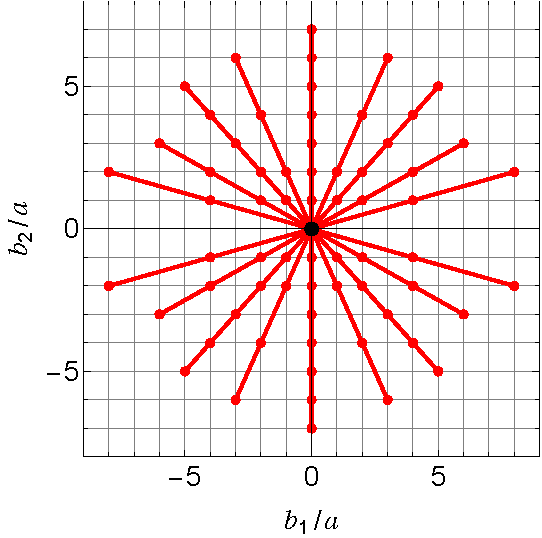
\includegraphics[width=\linewidth]{plots/kinematics_interpolation/bL_bT_plot.pdf}
        \caption{Caption for plot with path}
        \label{fig:bL_bT_path}
    \end{minipage}\hfill
    \begin{minipage}{0.45\textwidth}
        \centering
        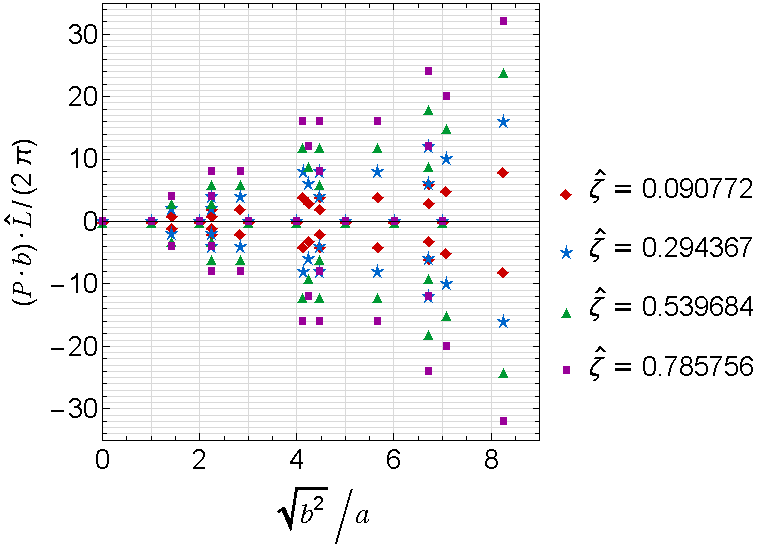
\includegraphics[width=\linewidth]{plots/kinematics_interpolation/Pb_bsq_plot.pdf}
        \caption{Caption for standard plot}
        \label{fig:bL_bT_standard}
    \end{minipage}
\end{figure}

\begin{figure}[h!]
    \centering
    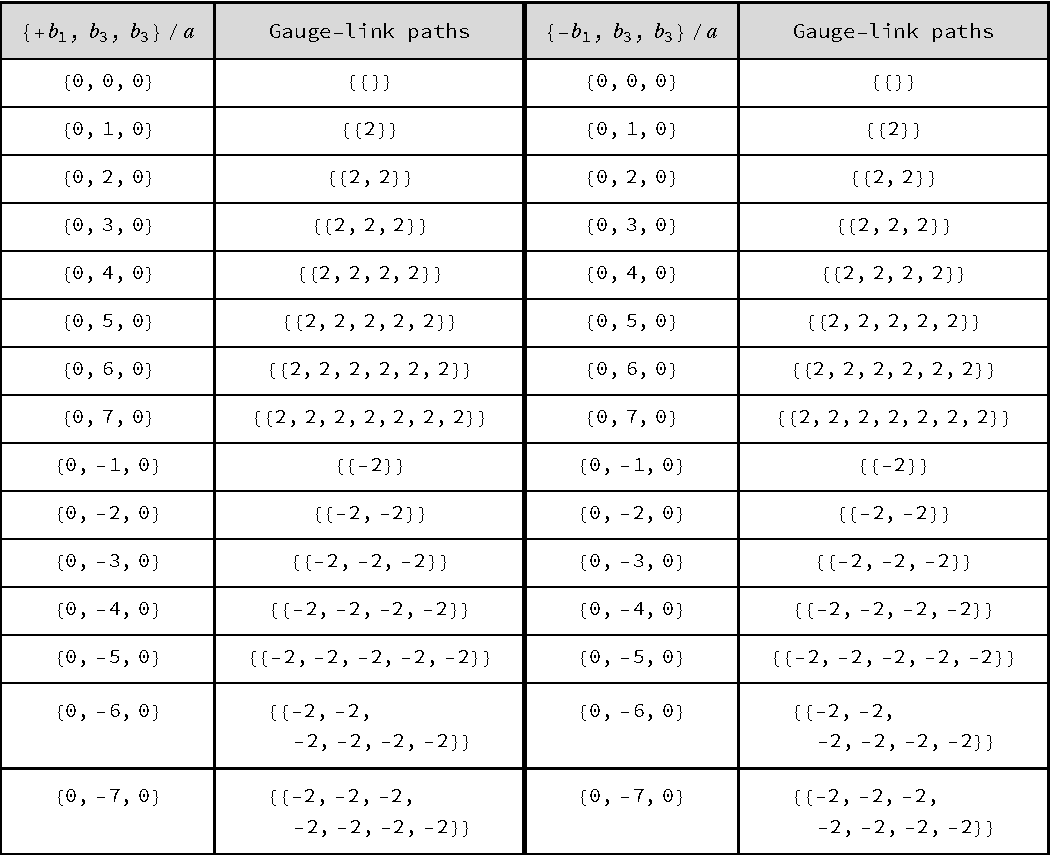
\includegraphics[width=0.5\linewidth]{plots/kinematics_interpolation/b_gauge_links_for_table1.pdf}
    \caption{Caption}
    \label{fig:placeholder}
\end{figure}
\begin{figure}[h!]
    \centering
    \begin{minipage}{0.45\textwidth}
        \centering
        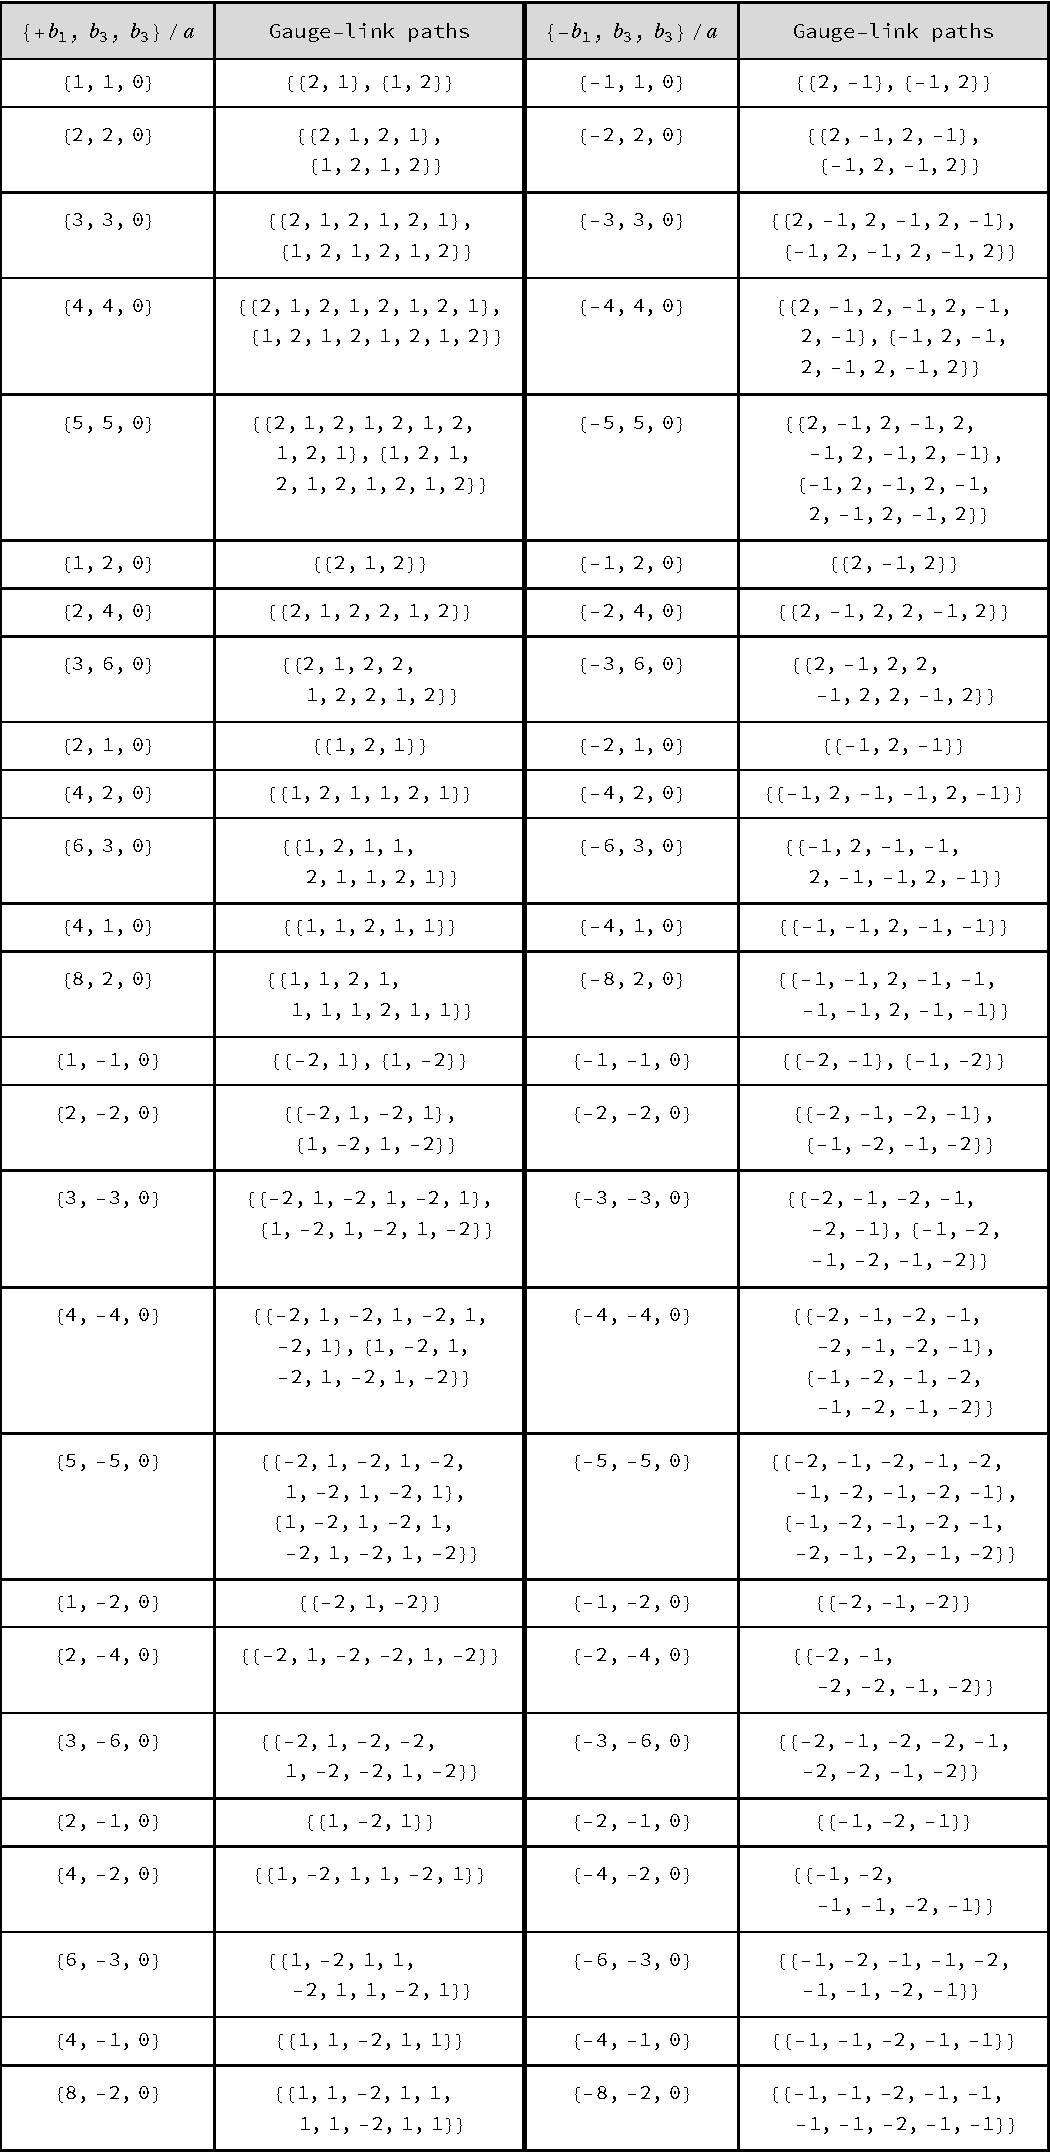
\includegraphics[width=\linewidth]{plots/kinematics_interpolation/b_gauge_links_for_table2.pdf}
        \caption{First caption}
        \label{fig:placeholder1}
    \end{minipage}\hfill
    \begin{minipage}{0.45\textwidth}
        \centering
        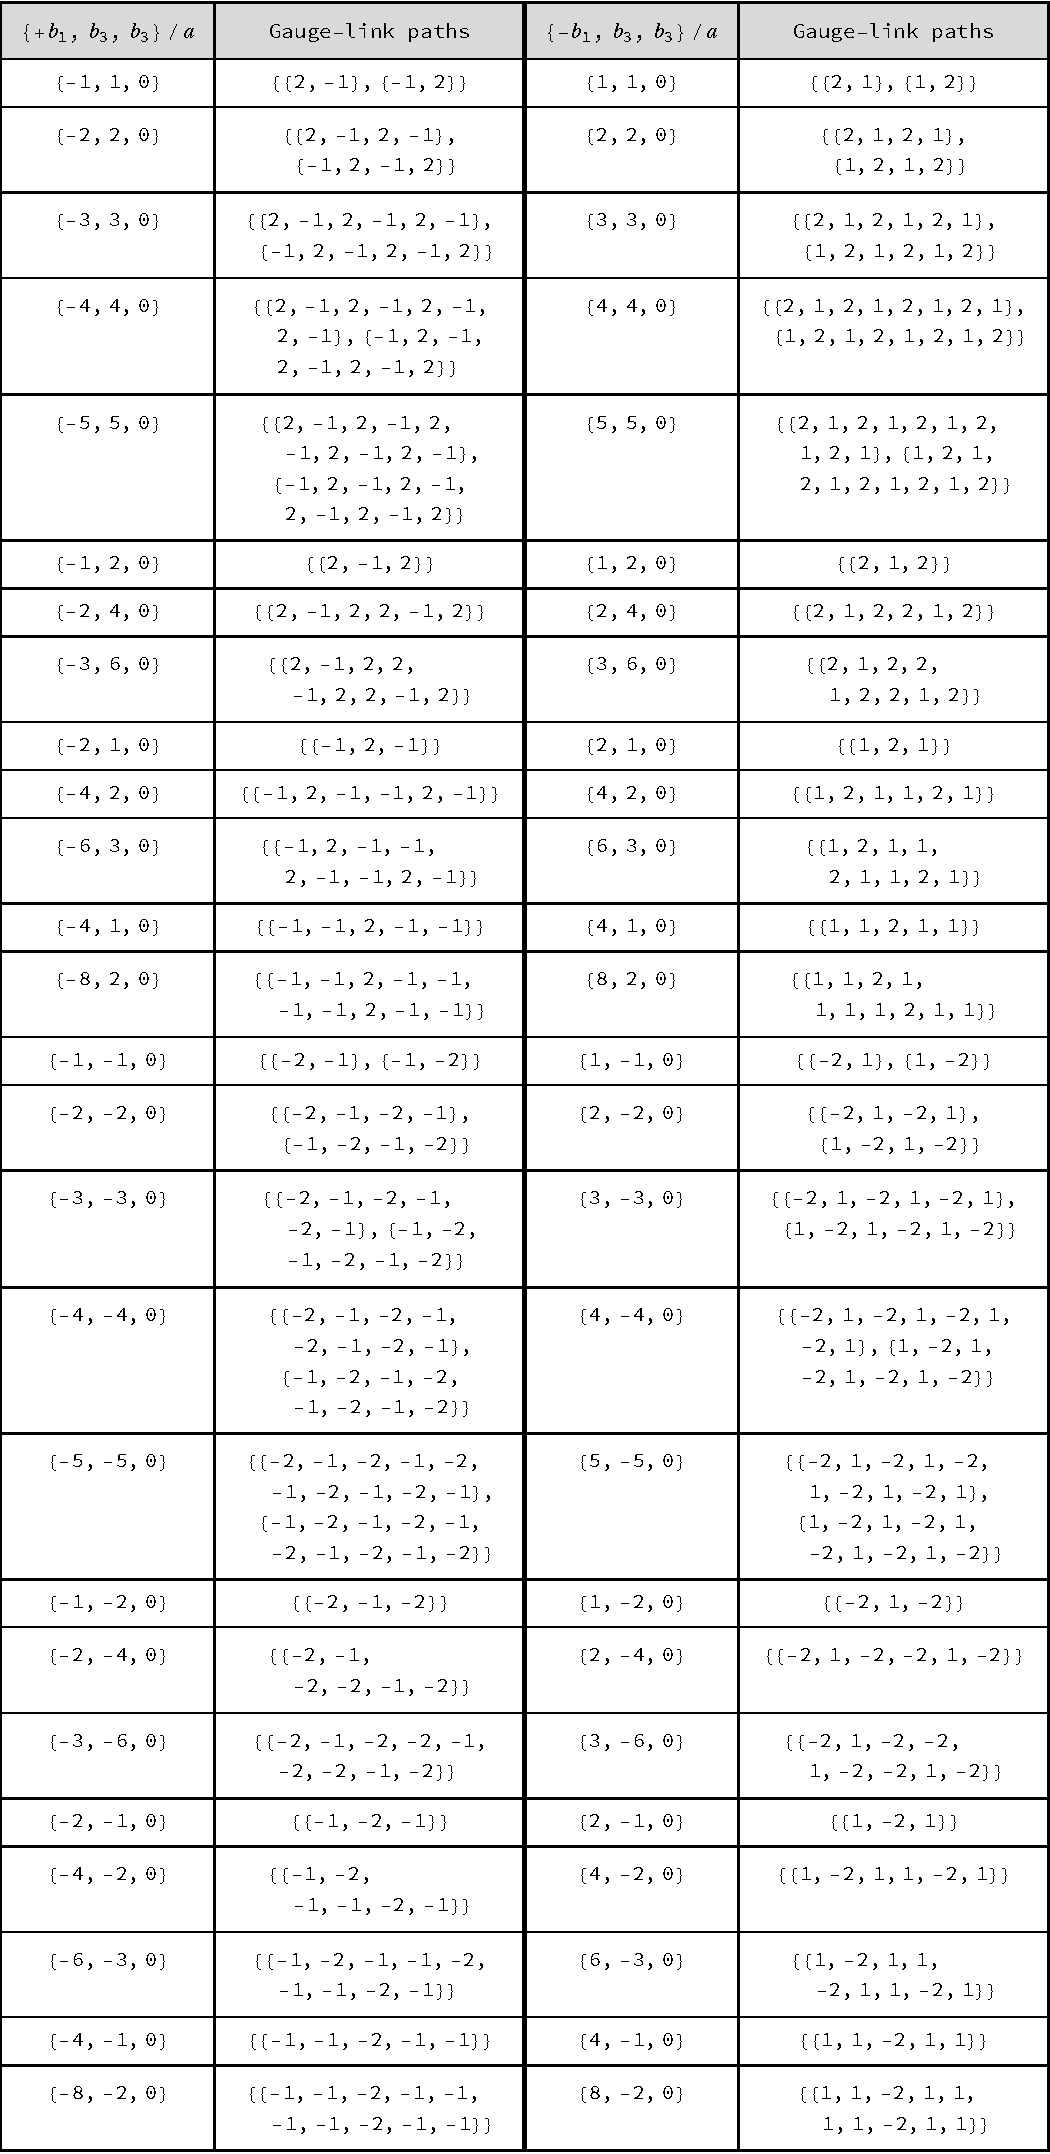
\includegraphics[width=\linewidth]{plots/kinematics_interpolation/b_gauge_links_for_table3.pdf}
        \caption{Second caption}
        \label{fig:placeholder2}
    \end{minipage}
\end{figure}

\pagebreak
Same $\vect{b}$ with different linkpaths are averaged
\begin{figure}[h!]
    \centering
    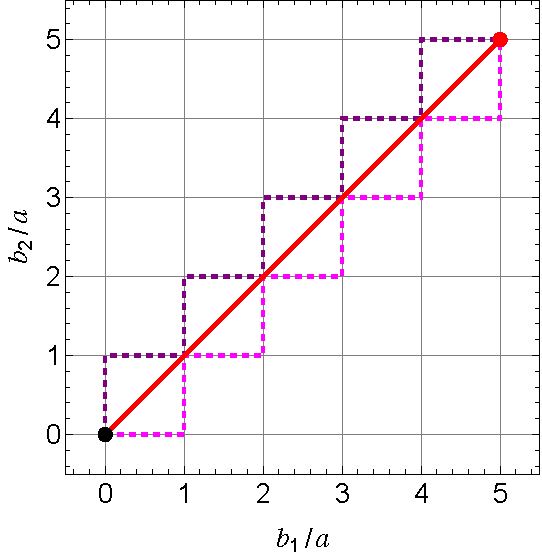
\includegraphics[width=0.3\linewidth]{plots/kinematics_interpolation/Example_b_plot_with_2path.pdf}
    \caption{Caption}
    \label{fig:placeholder}
\end{figure}
\begin{figure}[h!]
    \centering
    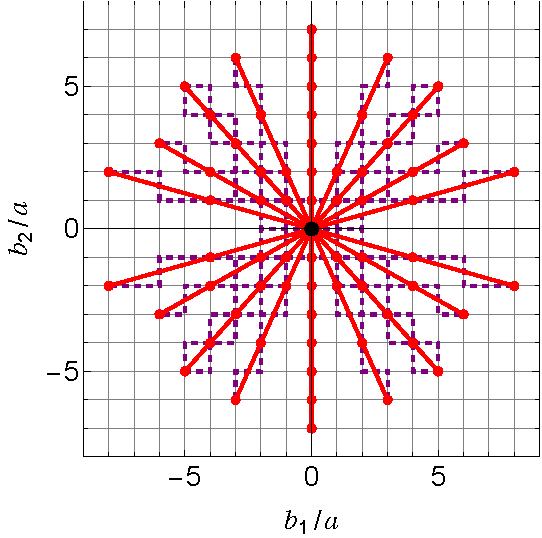
\includegraphics[width=0.5\linewidth]{plots/kinematics_interpolation/bL_bT_plot_with_path.pdf}
    \caption{Caption}
    \label{fig:placeholder}
\end{figure}

\pagebreak
\subsubsection{\texorpdfstring{$\vect{v}$}{TEXT} - Interpolation}
Same $\vect{v}$ with different sidelink are averaged
\begin{figure}[h!]
    \centering
    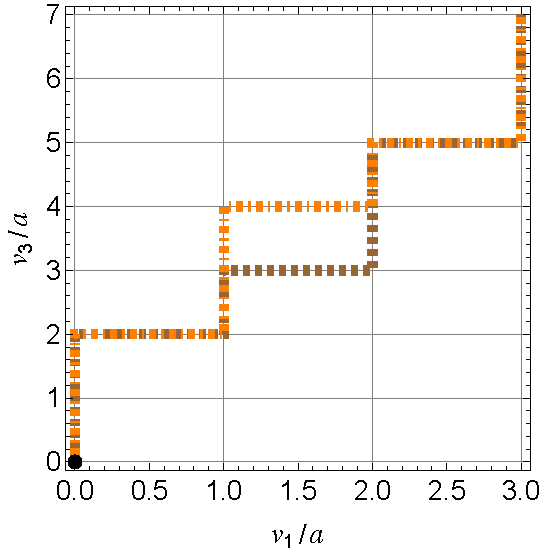
\includegraphics[width=0.5\linewidth]{plots/kinematics_interpolation/Example_v_plot_with_2path.pdf}
    \caption{Caption}
    \label{fig:placeholder}
\end{figure}
\begin{figure}[h!]
    \centering
    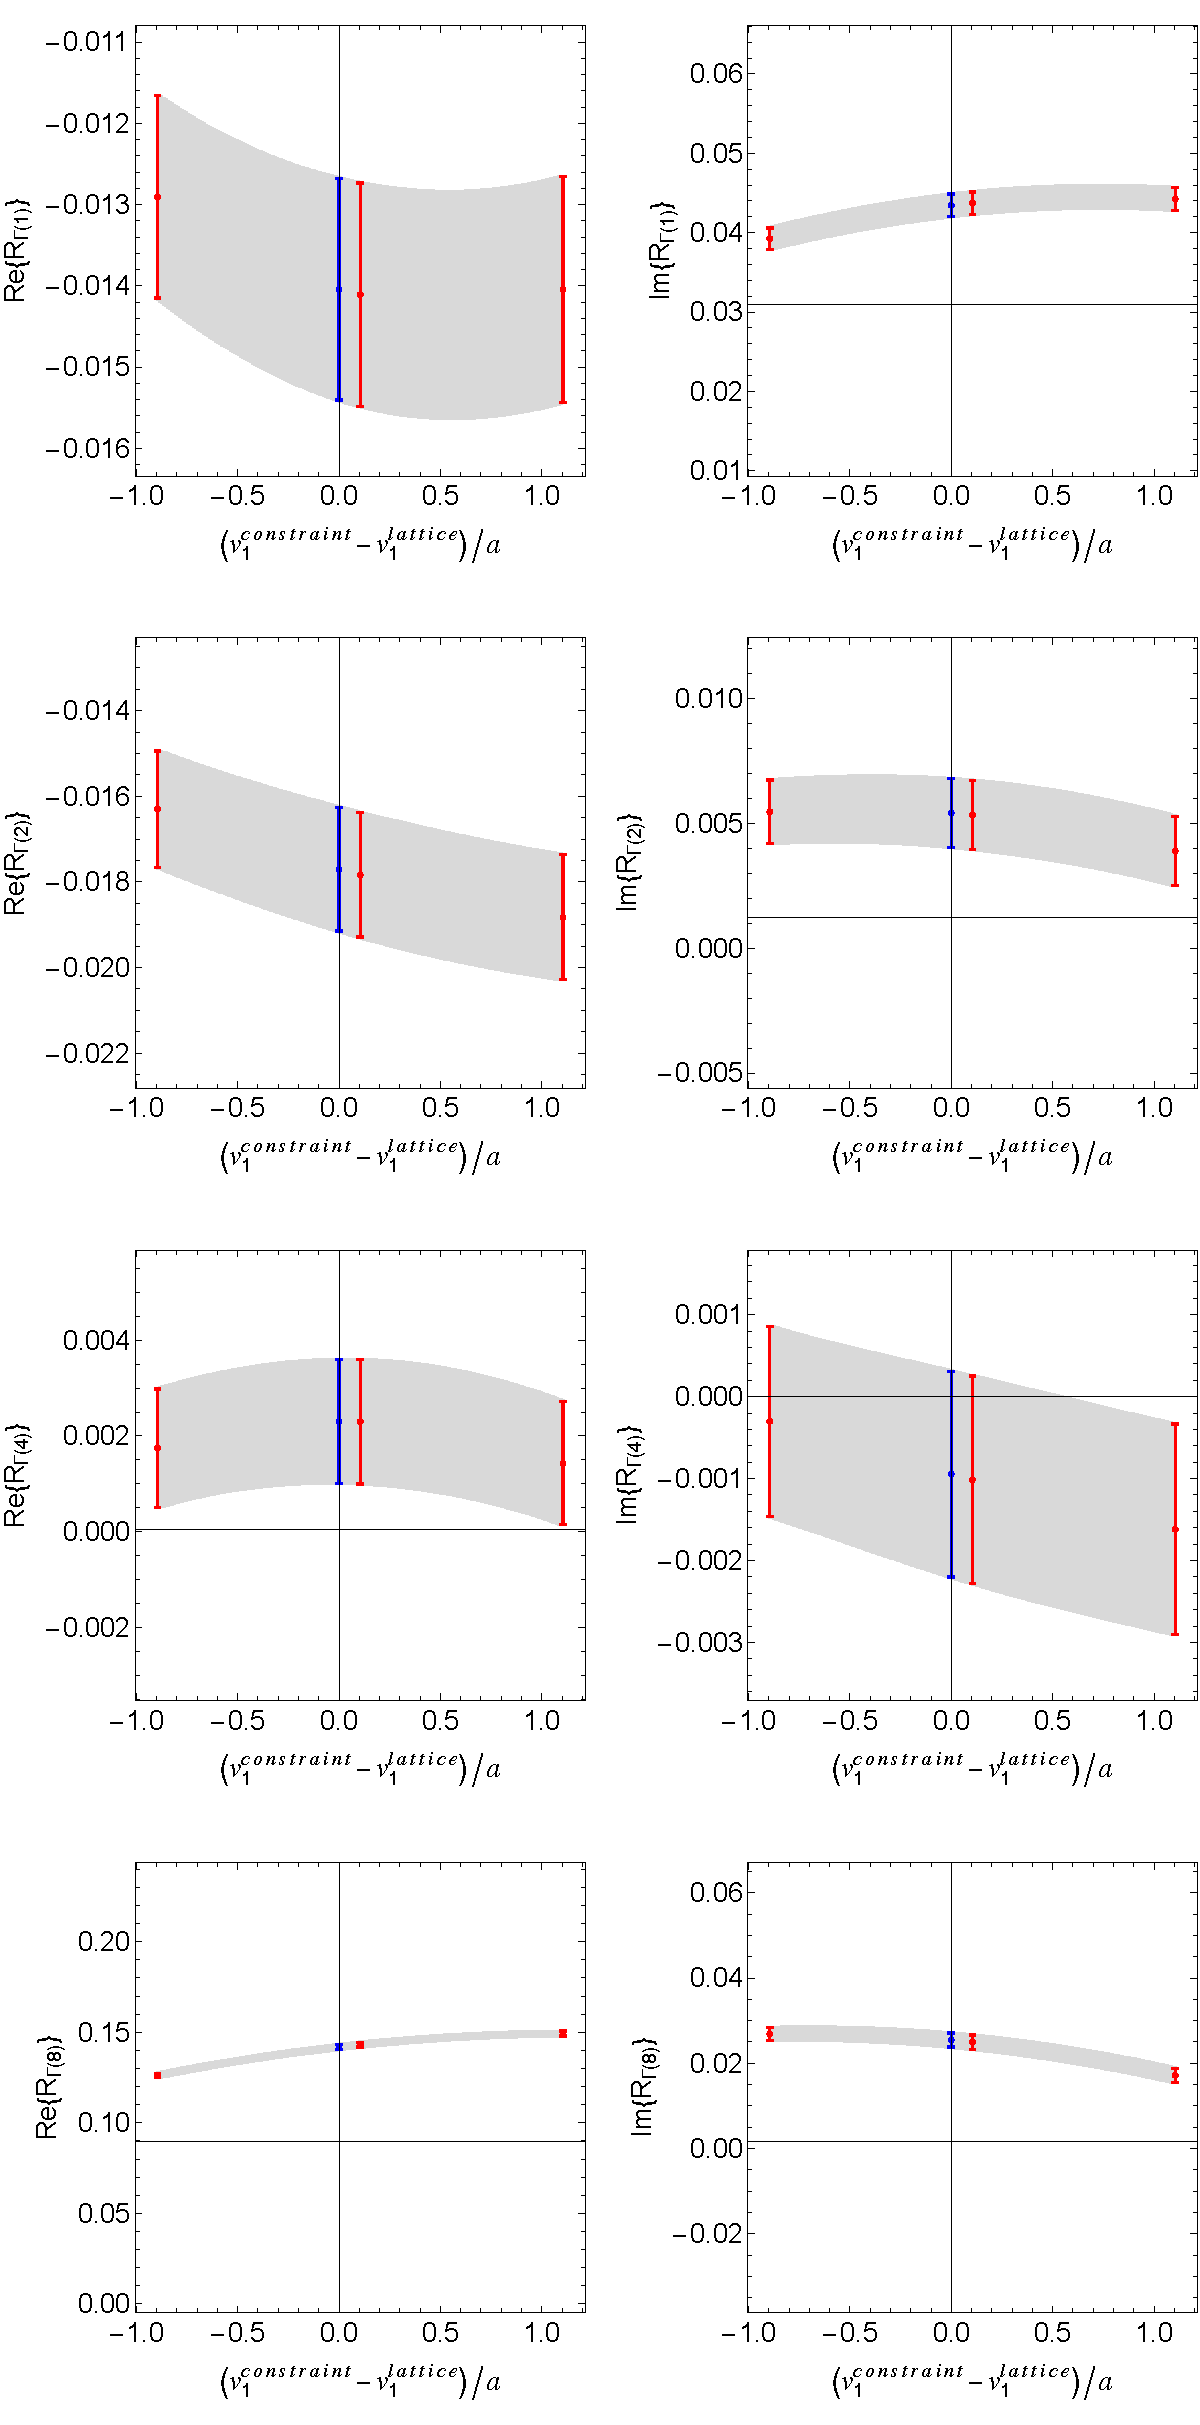
\includegraphics[width=0.6\linewidth]{plots/kinematics_interpolation/Interpolation_Ex_b120_eta7_P-1.pdf}
    \caption{Interpolation Example for $\vect{b}={1,2,0}$, $\eta=7$, $P_L\cdot a\hat{L}/(2\pi)=-1$}
    \label{fig:placeholder}
\end{figure}

\pagebreak
\subsection{Lattice calculations of Amplitudes}
\subsubsection{\texorpdfstring{$\hat{\zeta}=0.090772$}{TEXT}}
\begin{figure}
    \centering
    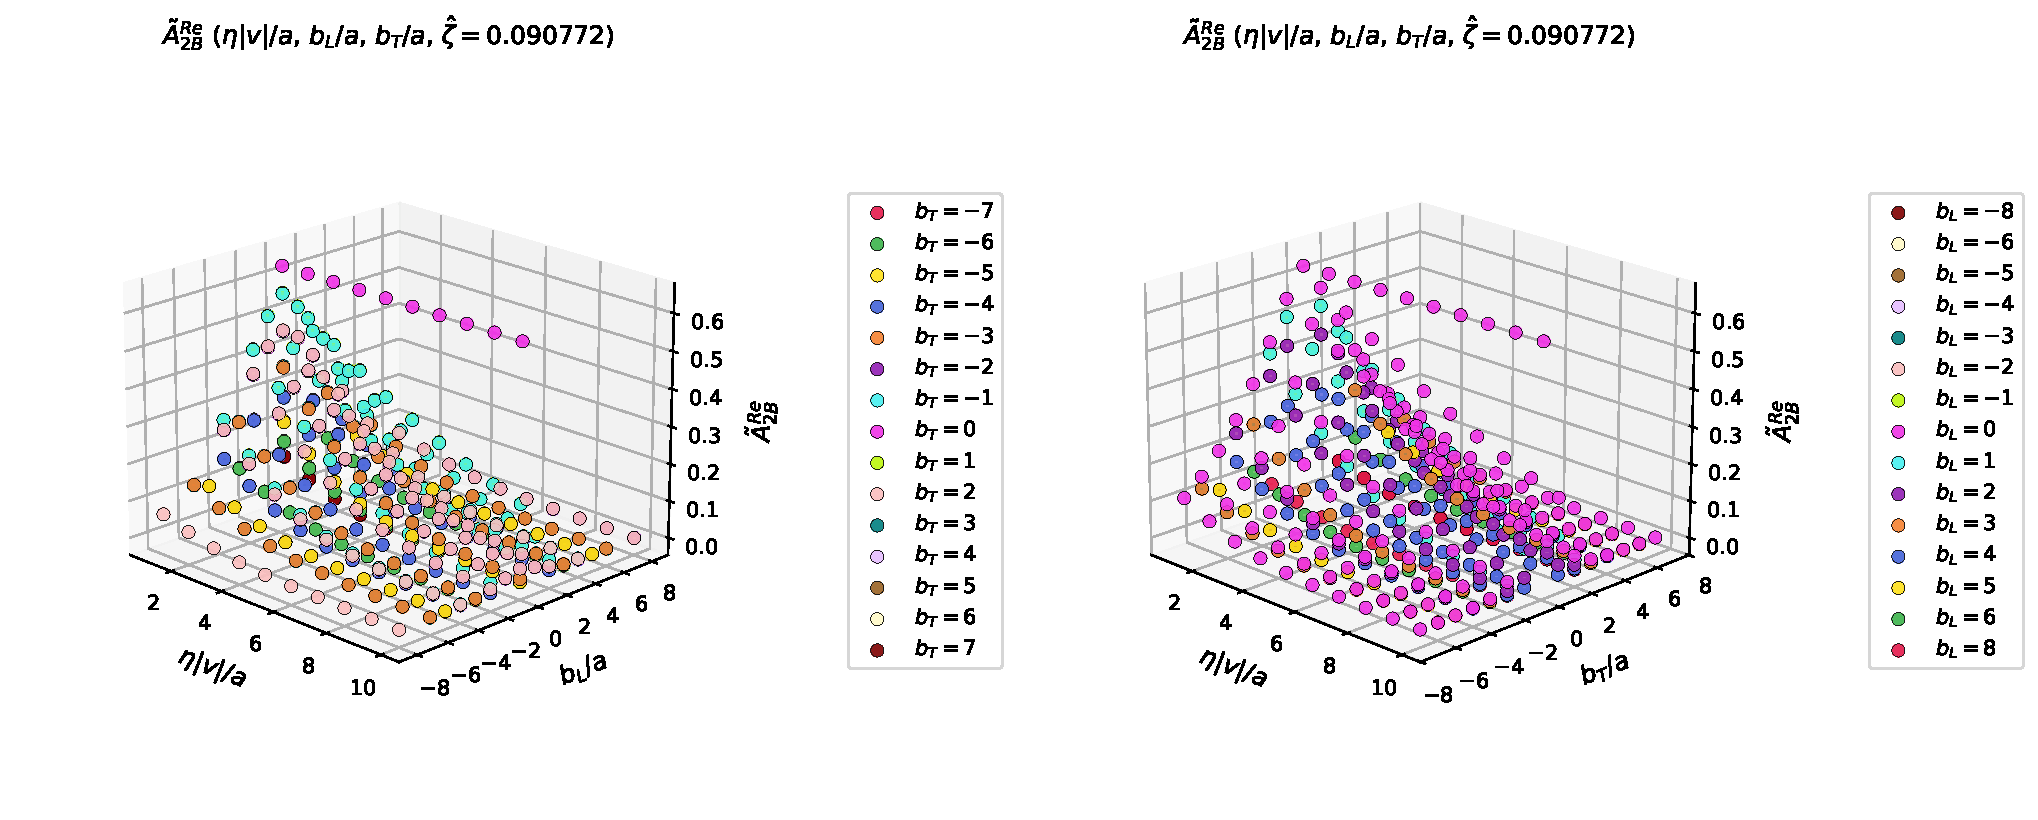
\includegraphics[width=0.7\linewidth]{plots/Amps_bL_bT/ReA2B_PL-1_3D.pdf}
    \caption{Caption}
    \label{fig:placeholder}
\end{figure}
\begin{figure}
    \centering
    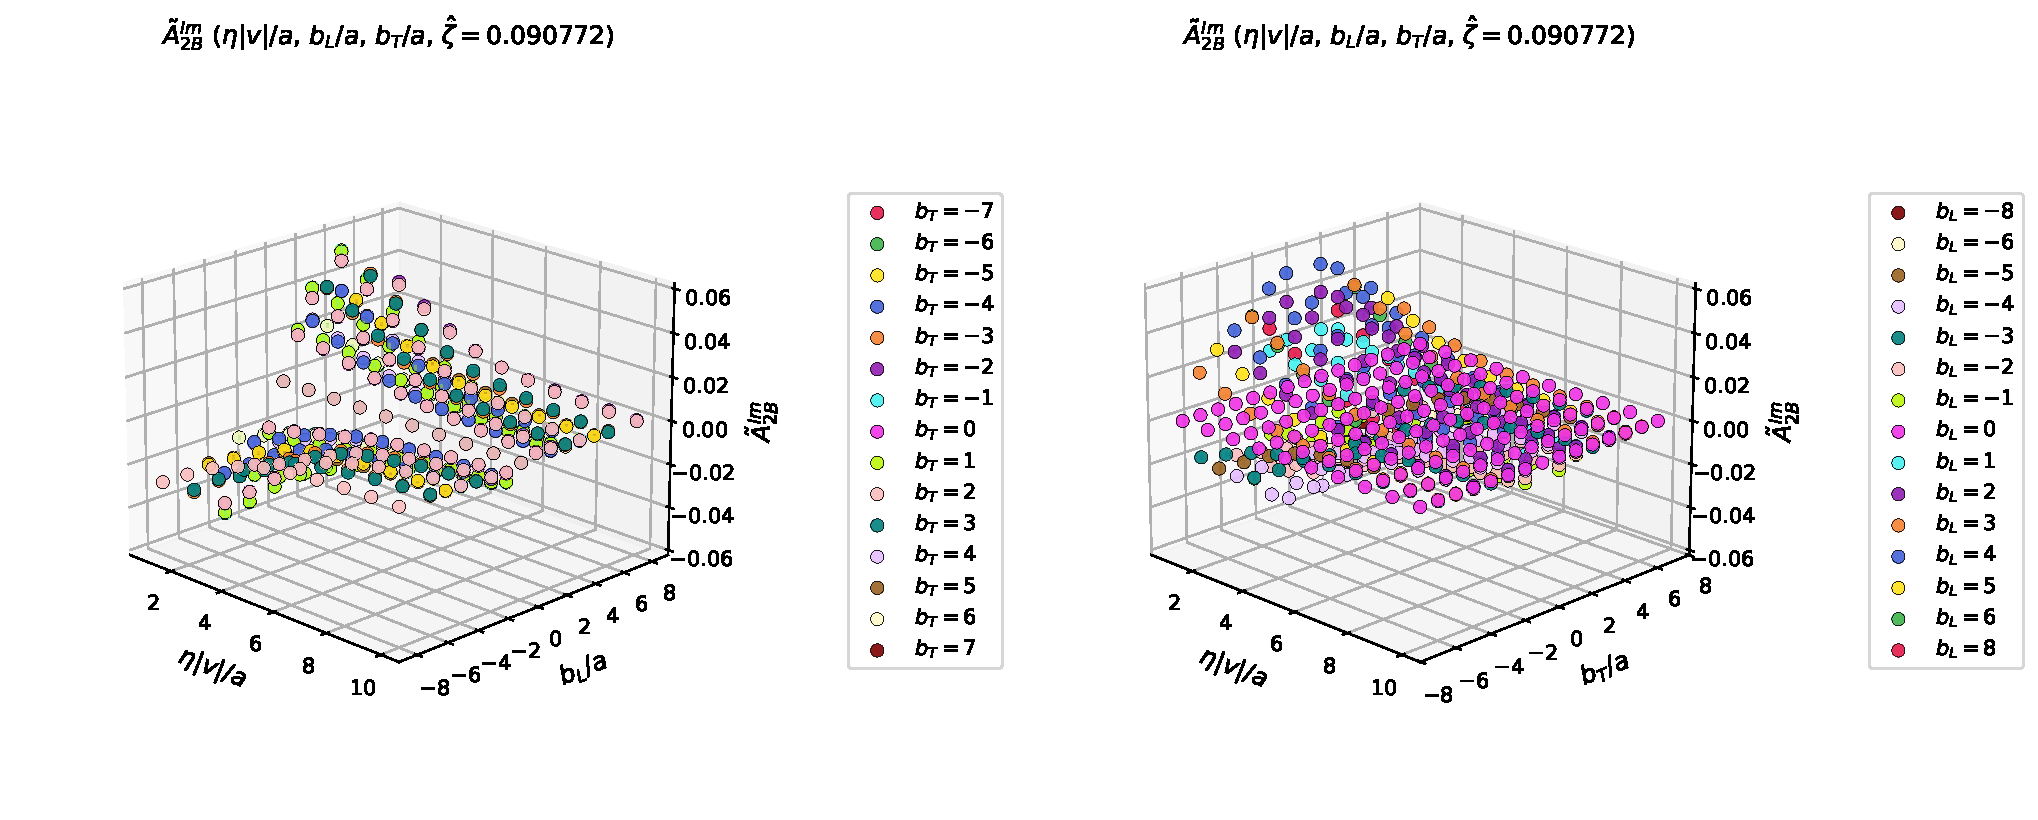
\includegraphics[width=0.7\linewidth]{plots/Amps_bL_bT/ImA2B_PL-1_3D.pdf}
    \caption{Caption}
    \label{fig:placeholder}
\end{figure}
\begin{figure}
    \centering
    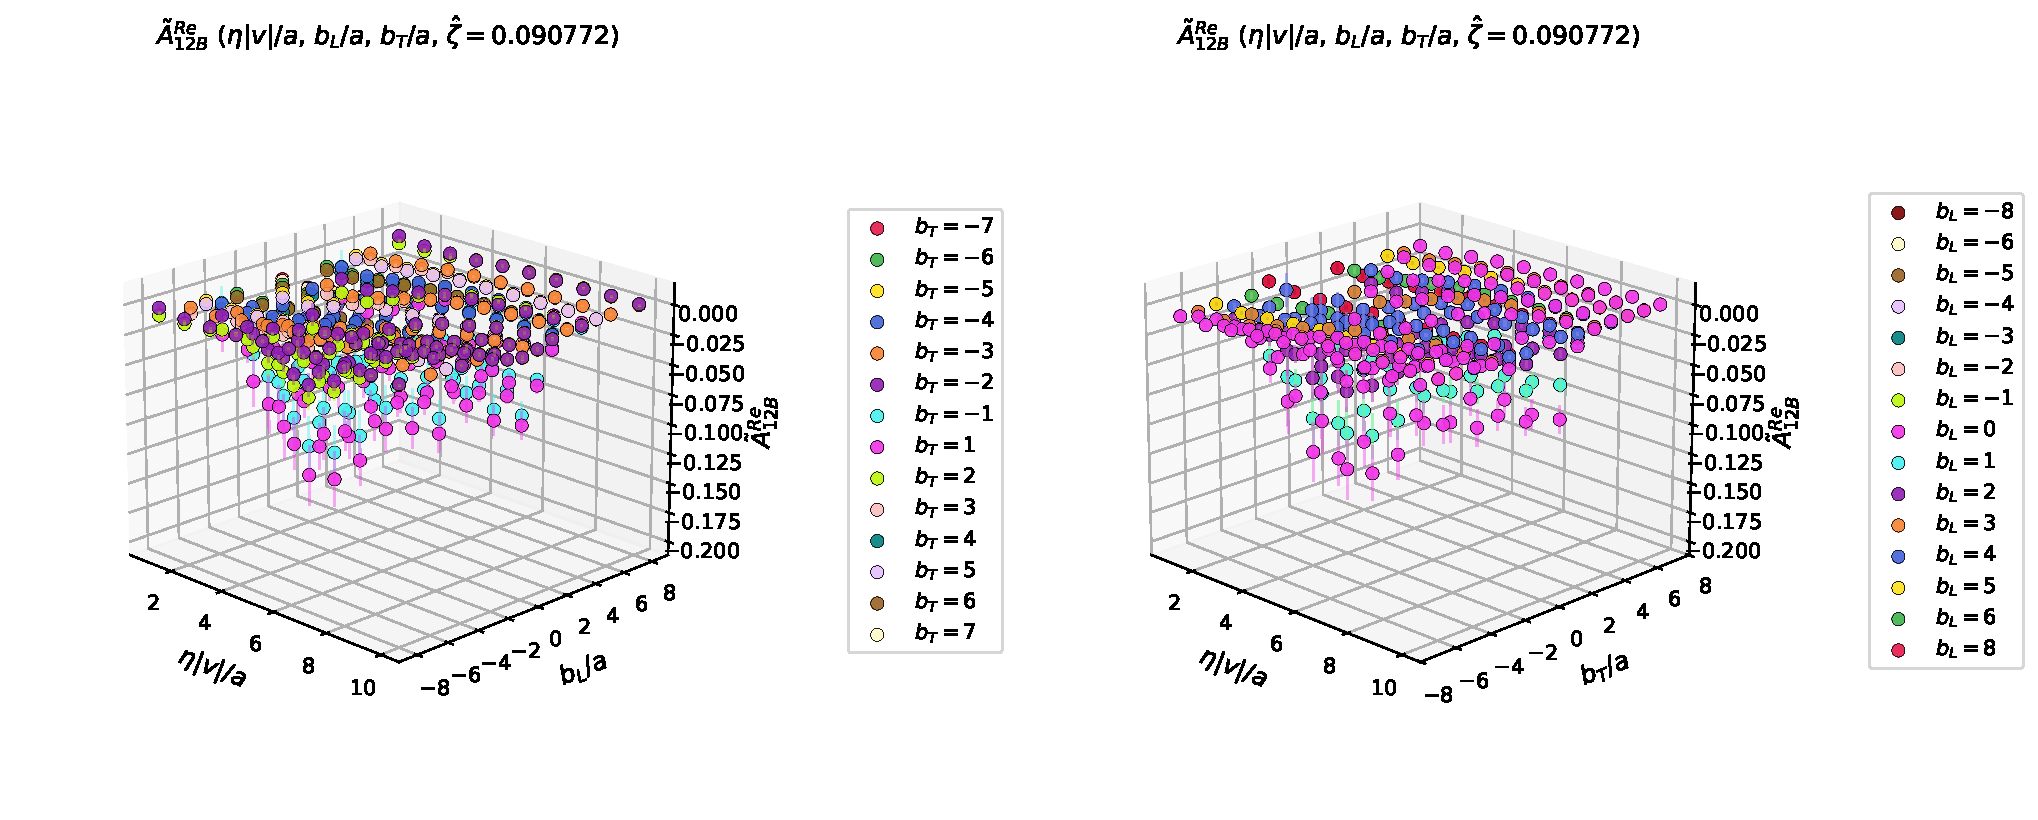
\includegraphics[width=0.7\linewidth]{plots/Amps_bL_bT/ReA12B_PL-1_3D.pdf}
    \caption{Caption}
    \label{fig:placeholder}
\end{figure}
\begin{figure}
    \centering
    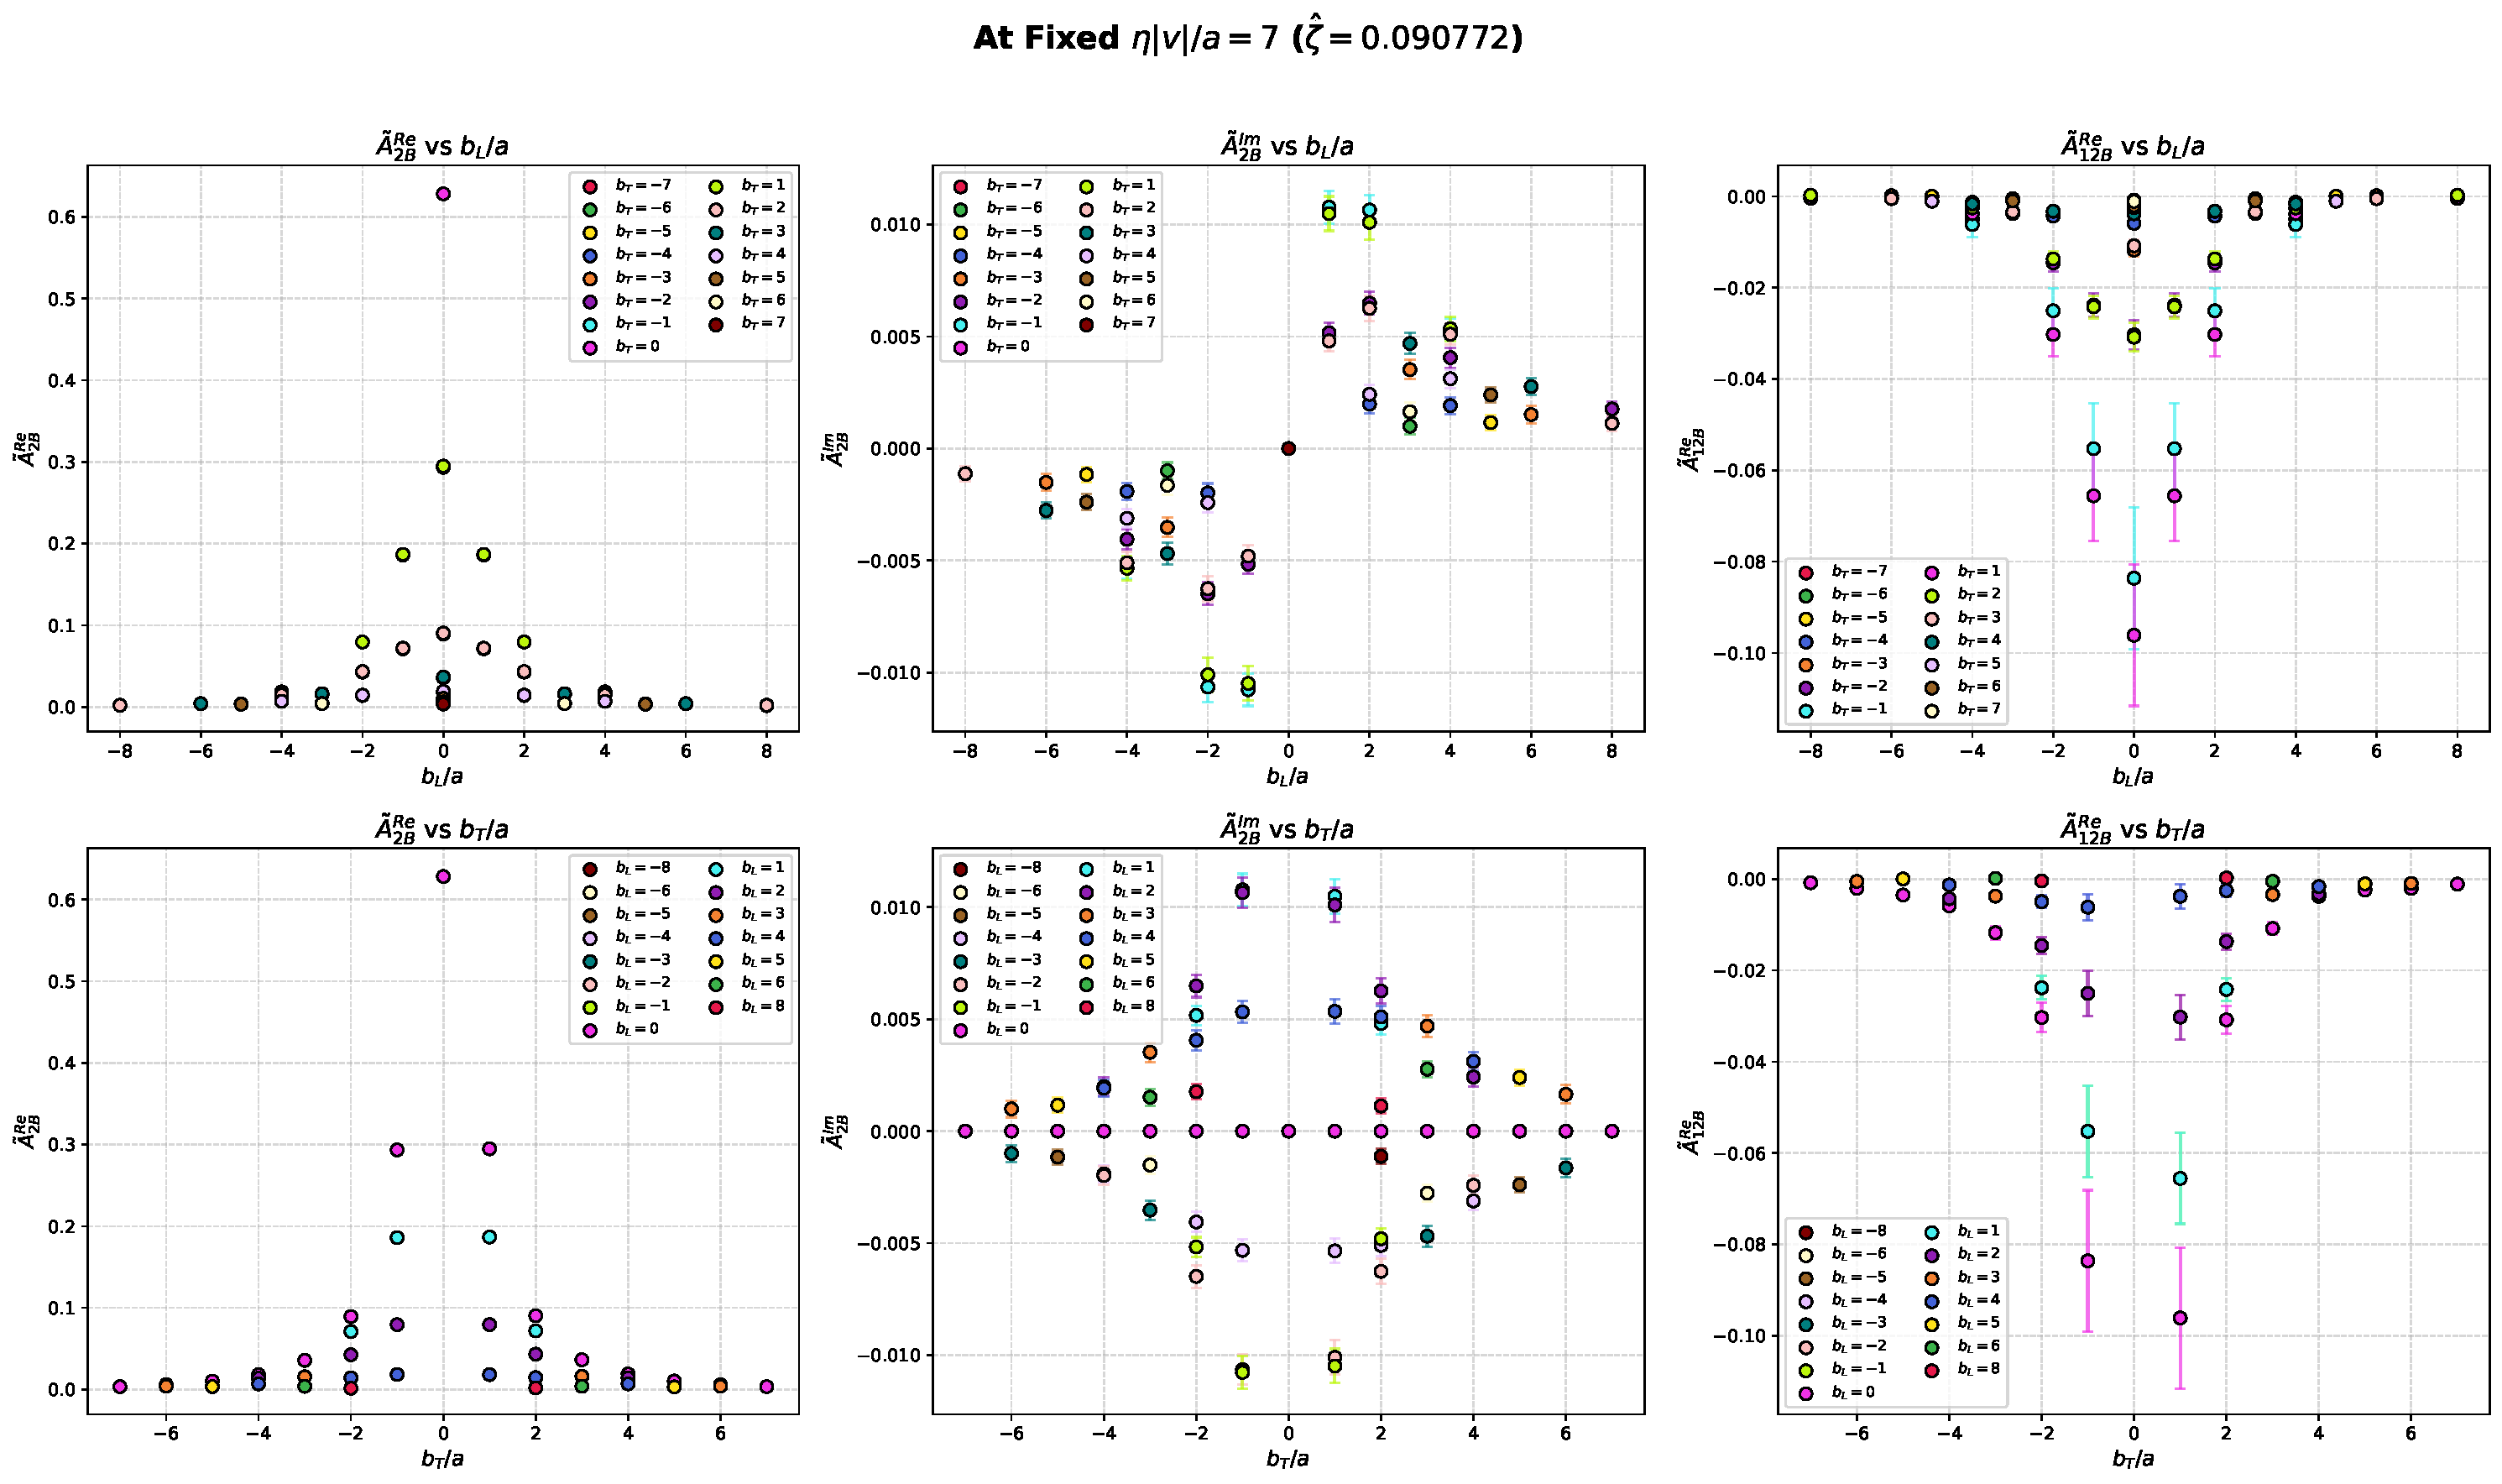
\includegraphics[width=0.7\linewidth]{plots/Amps_bL_bT/Combined_2D_eta7_PL-1.pdf}
    \caption{Caption}
    \label{fig:placeholder}
\end{figure}

\pagebreak
\subsubsection{\texorpdfstring{$\hat{\zeta}=0.294367$}{TEXT}}
\begin{figure}
    \centering
    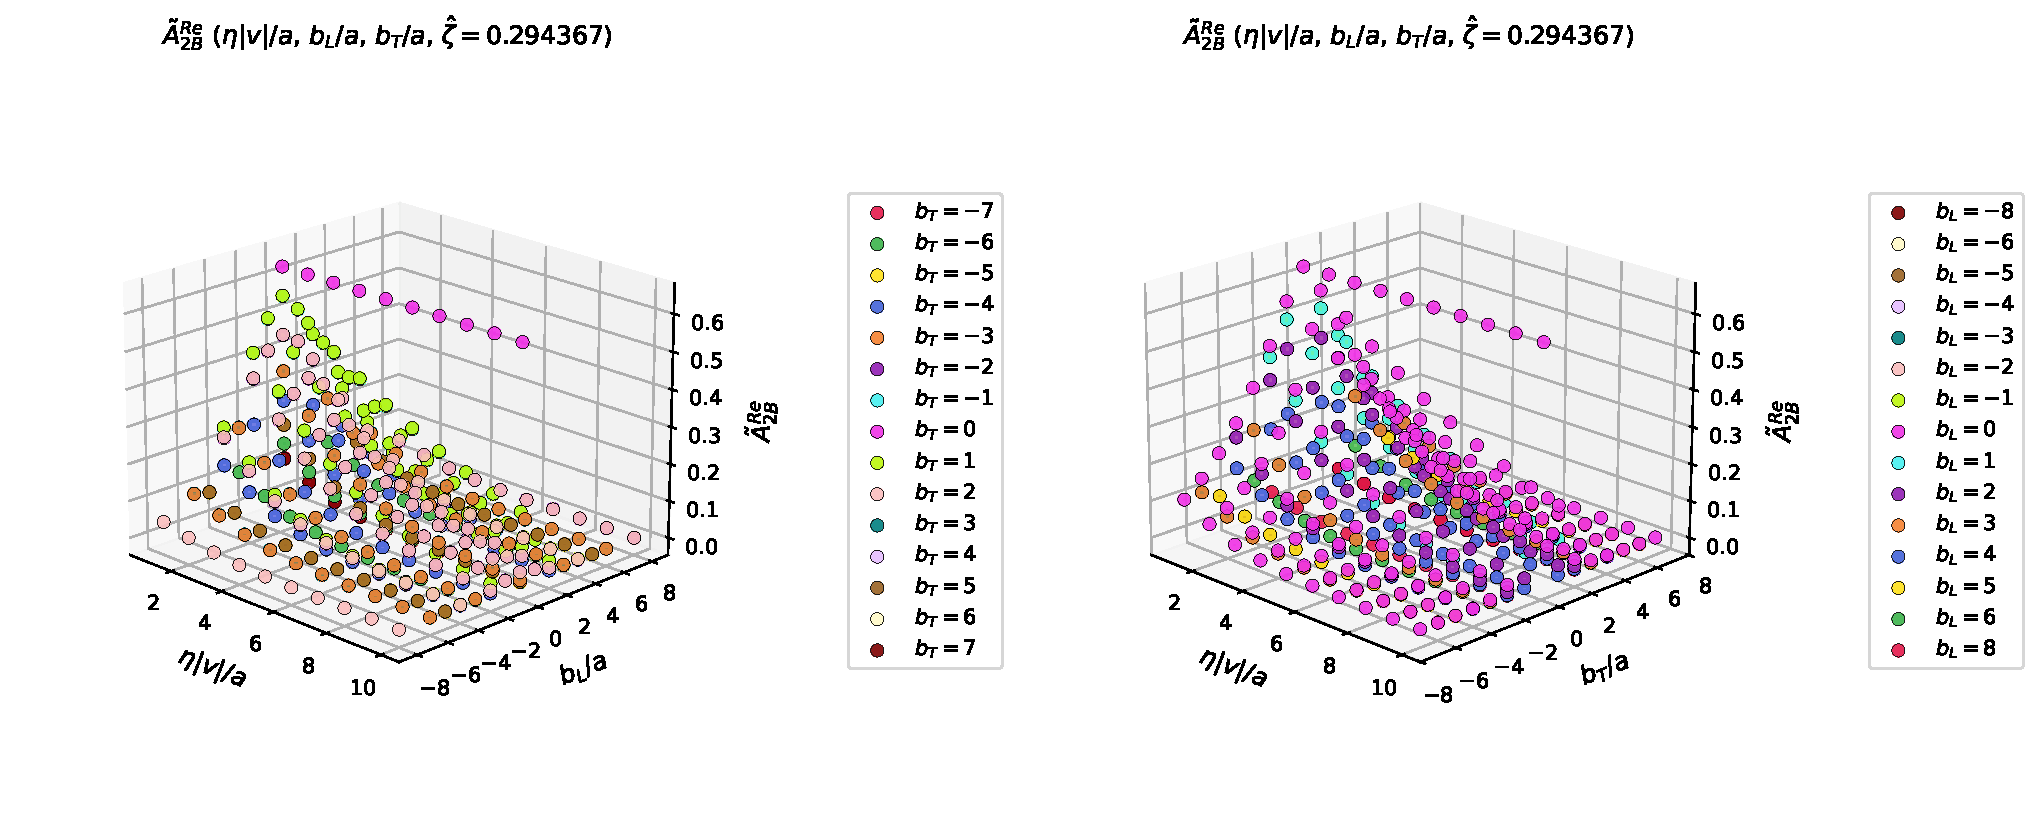
\includegraphics[width=0.7\linewidth]{plots/Amps_bL_bT/ReA2B_PL-2_3D.pdf}
    \caption{Caption}
    \label{fig:placeholder}
\end{figure}
\begin{figure}
    \centering
    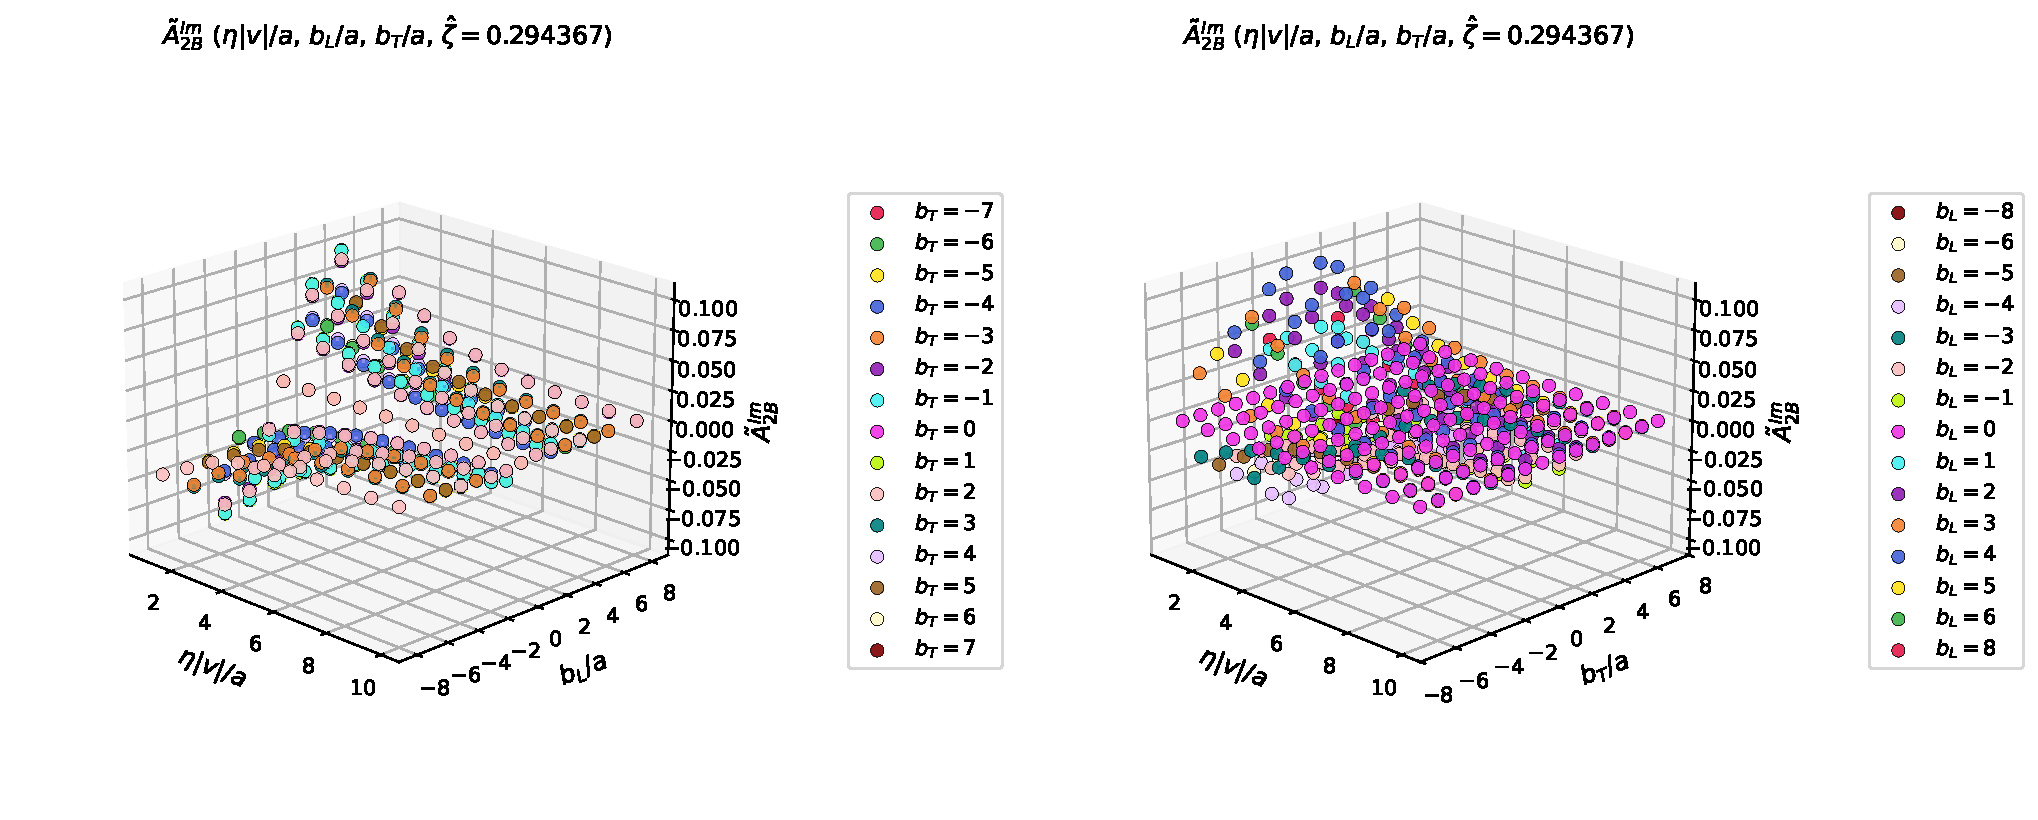
\includegraphics[width=0.7\linewidth]{plots/Amps_bL_bT/ImA2B_PL-2_3D.pdf}
    \caption{Caption}
    \label{fig:placeholder}
\end{figure}
\begin{figure}
    \centering
    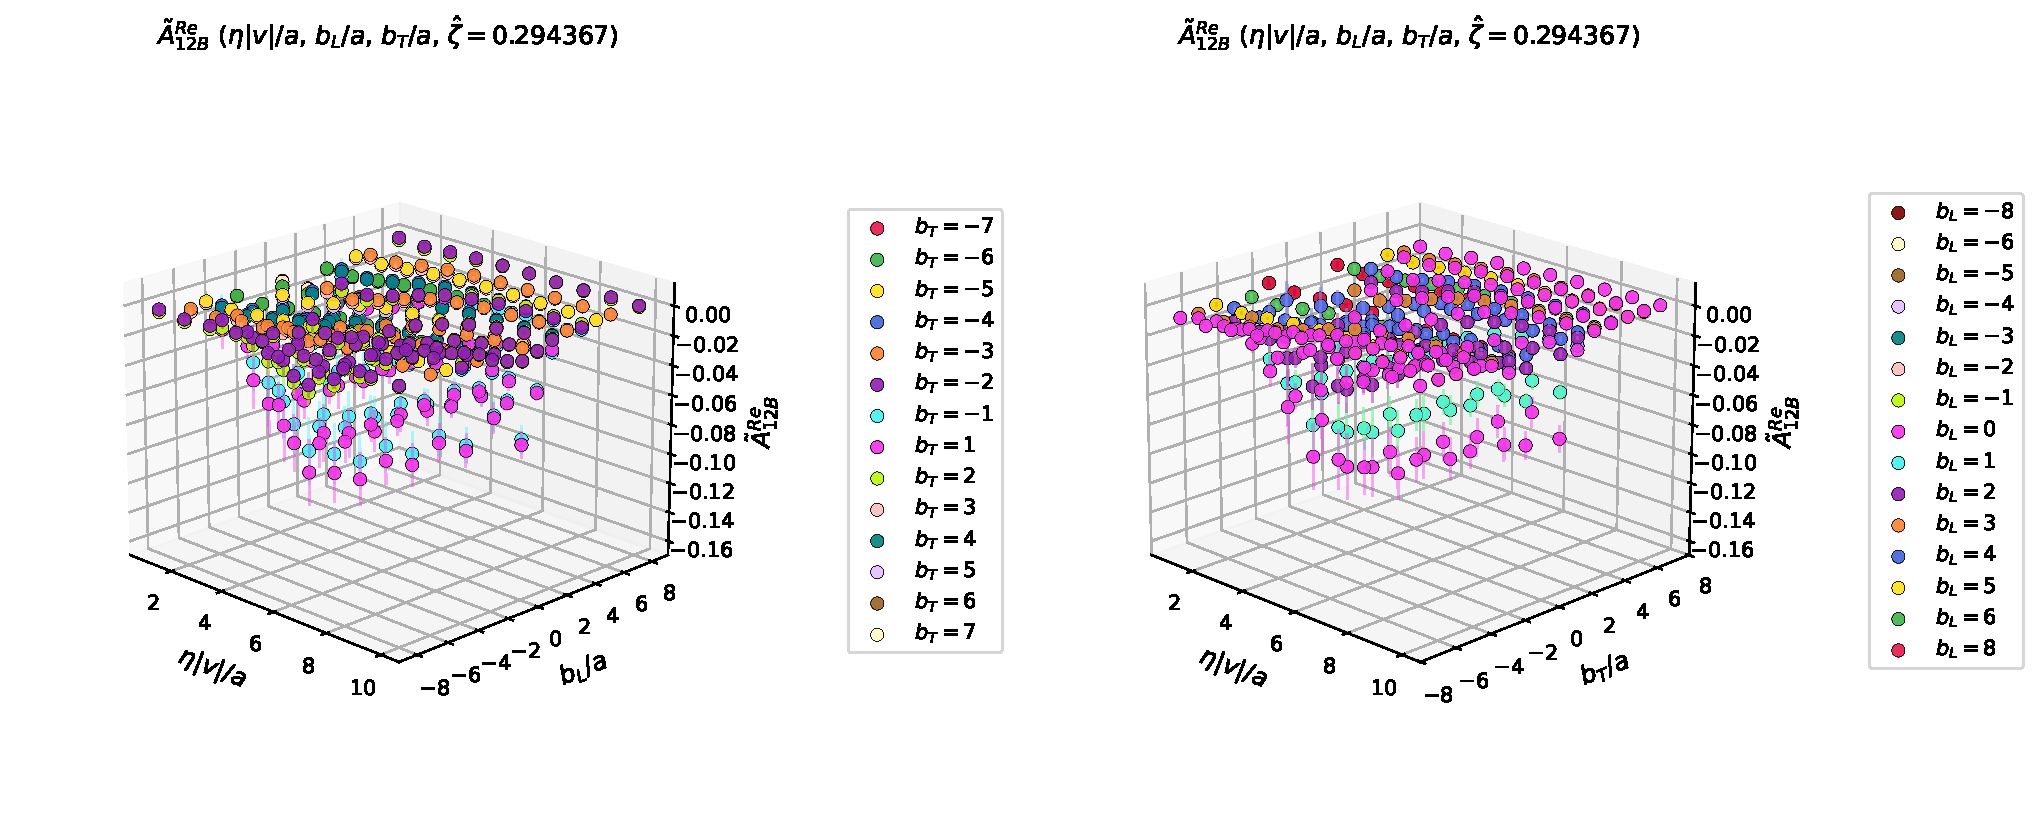
\includegraphics[width=0.7\linewidth]{plots/Amps_bL_bT/ReA12B_PL-2_3D.pdf}
    \caption{Caption}
    \label{fig:placeholder}
\end{figure}
\begin{figure}
    \centering
    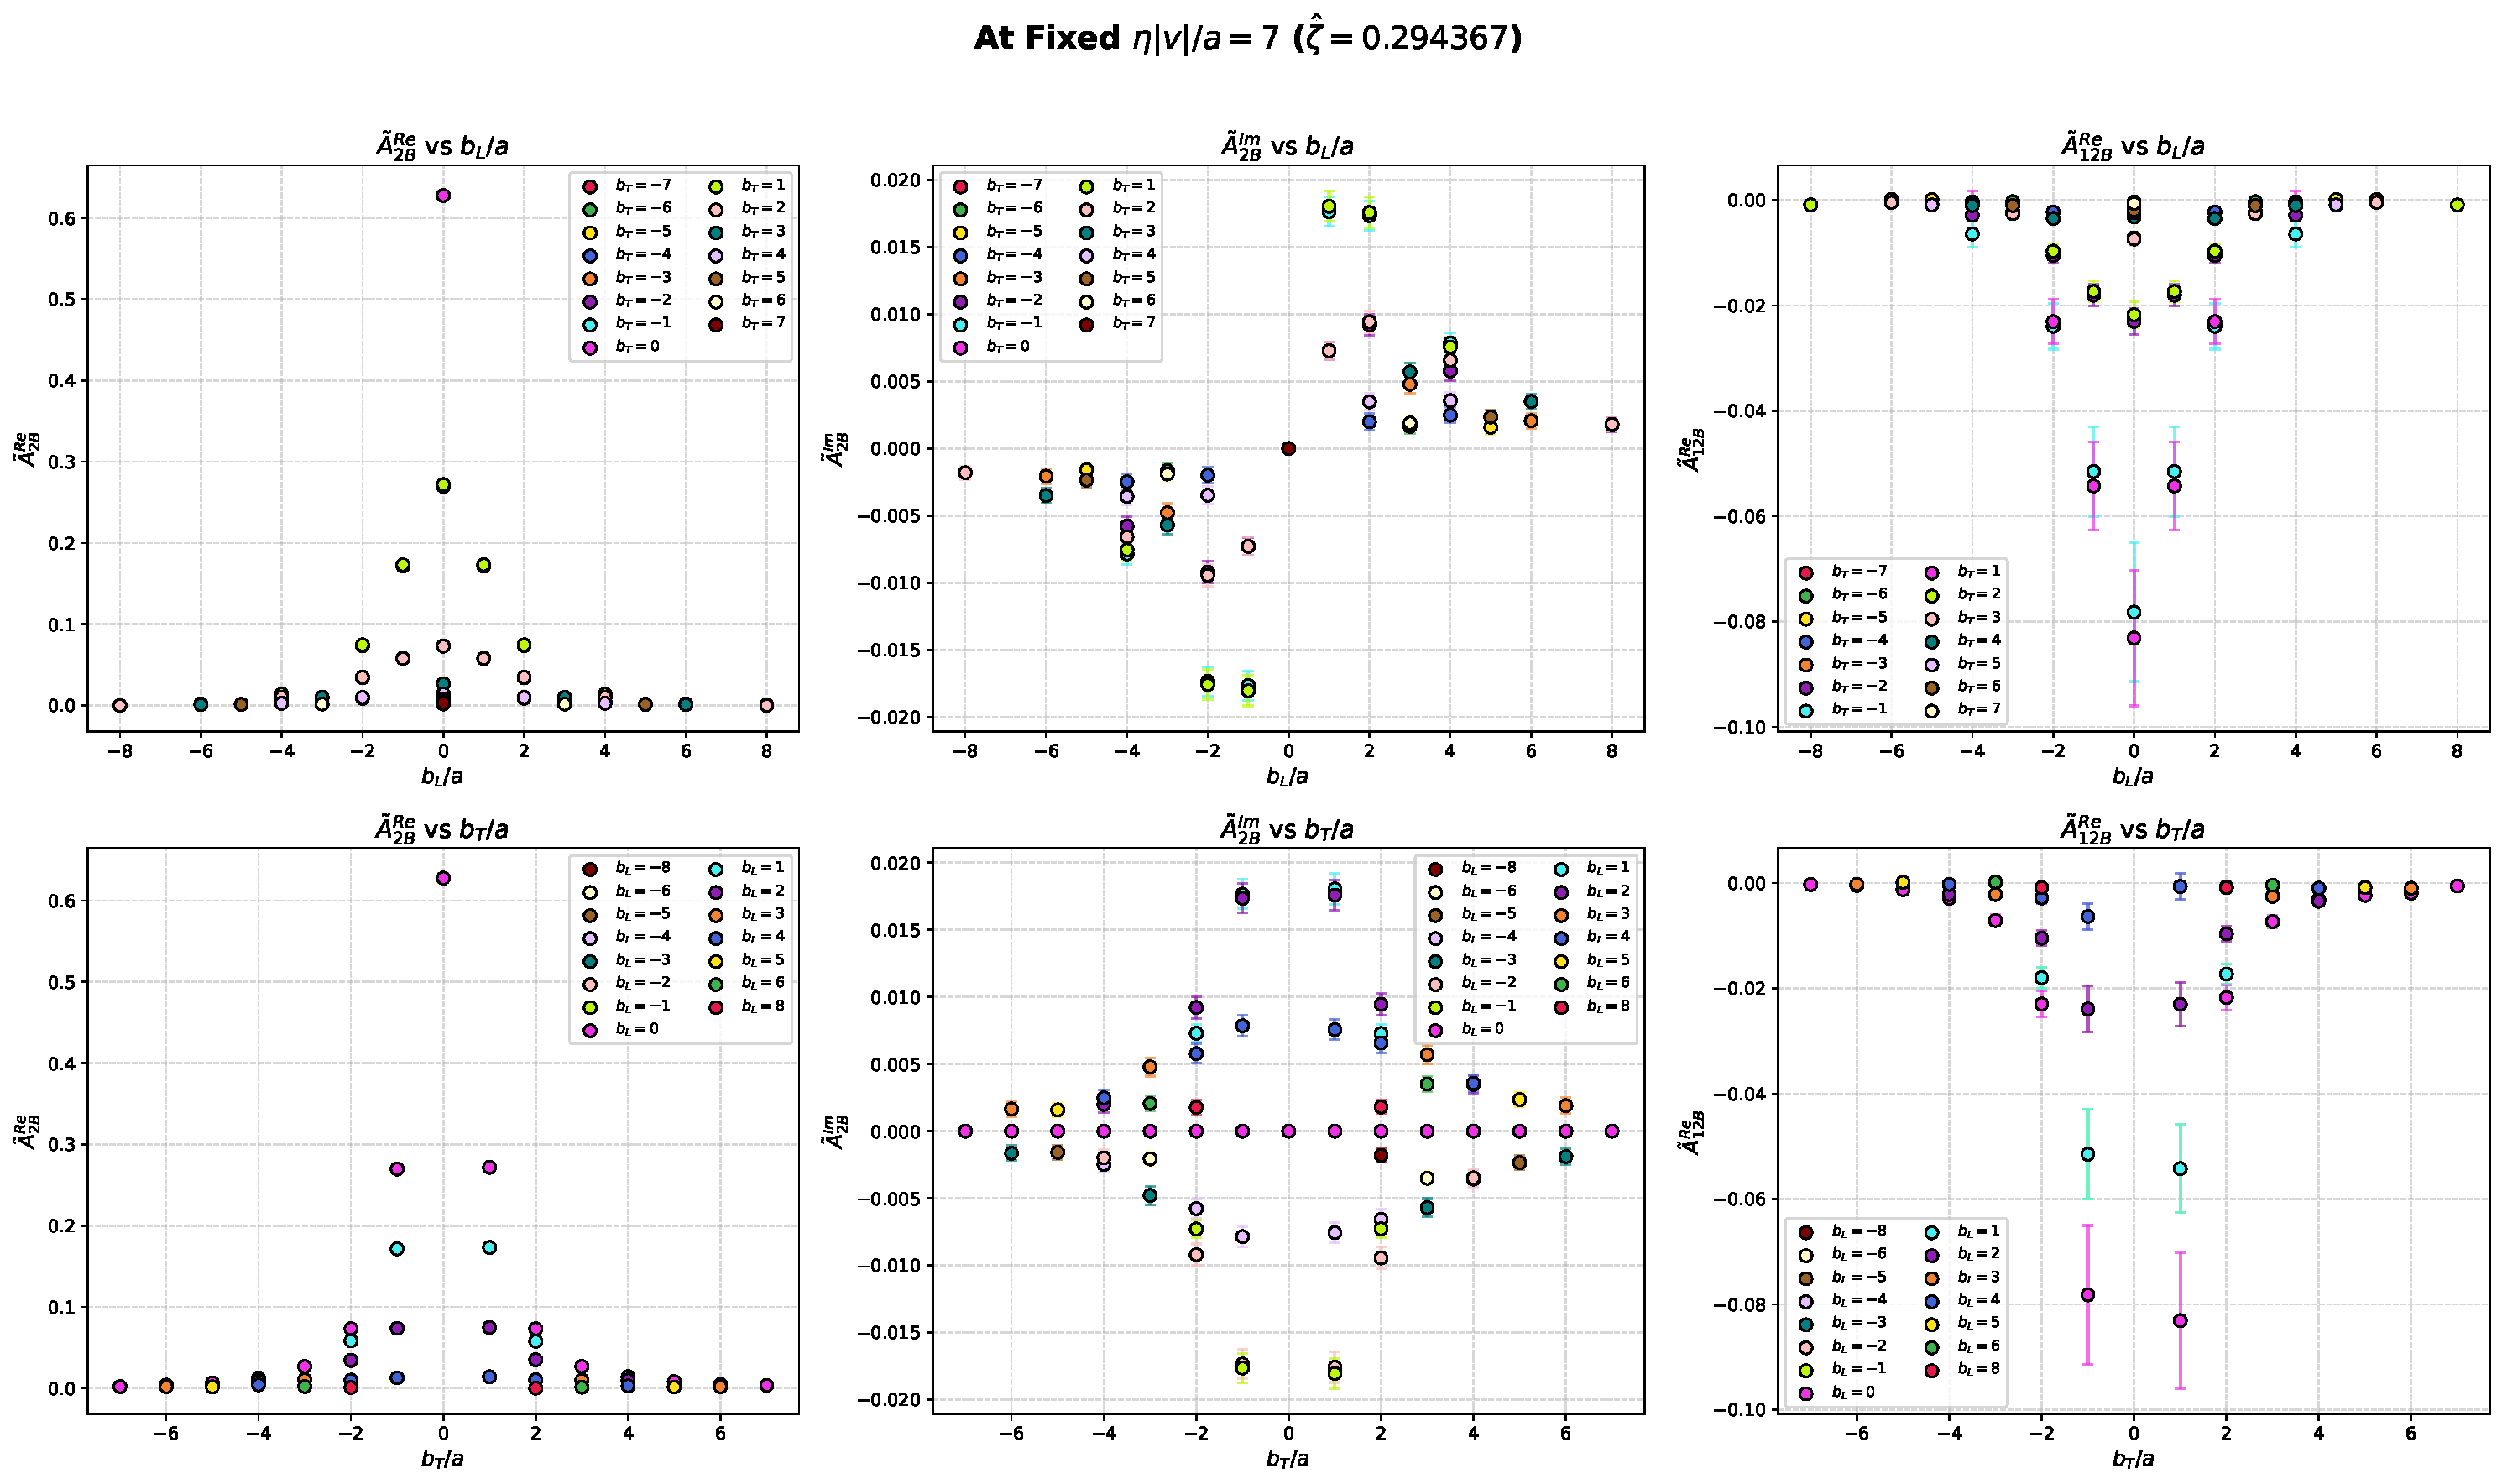
\includegraphics[width=0.7\linewidth]{plots/Amps_bL_bT/Combined_2D_eta7_PL-2.pdf}
    \caption{Caption}
    \label{fig:placeholder}
\end{figure}

\pagebreak
\subsubsection{\texorpdfstring{$\hat{\zeta}=0.539684$}{TEXT}}
\begin{figure}
    \centering
    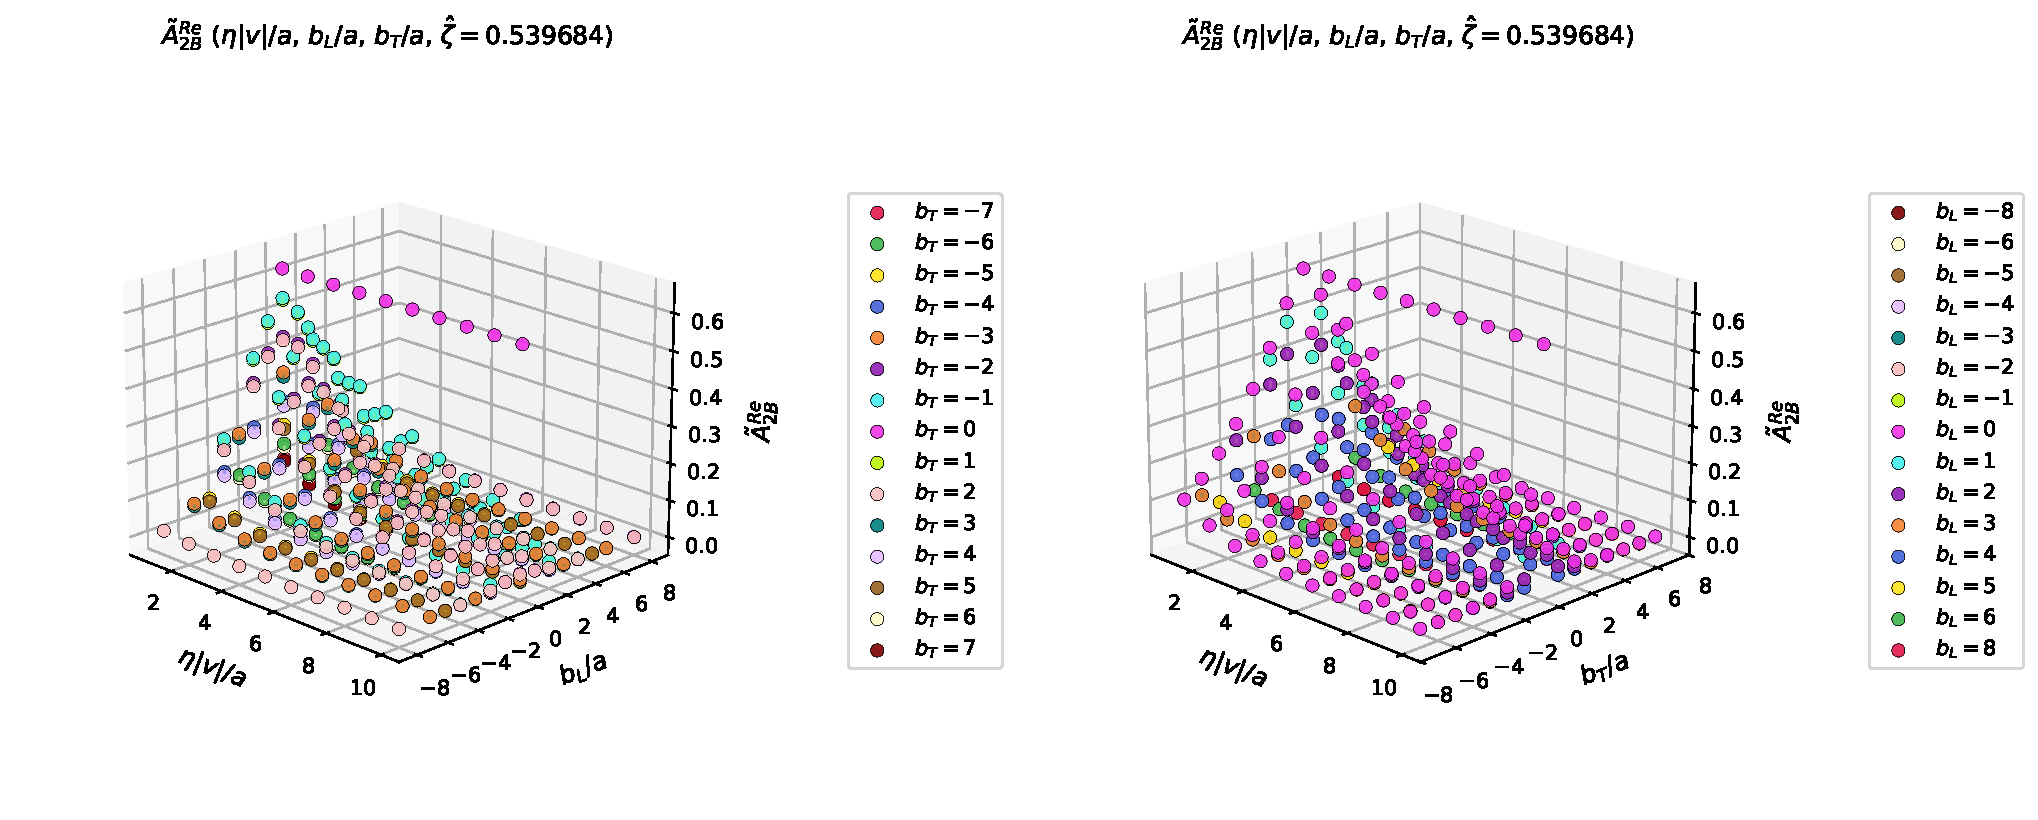
\includegraphics[width=0.7\linewidth]{plots/Amps_bL_bT/ReA2B_PL-3_3D.pdf}
    \caption{Caption}
    \label{fig:placeholder}
\end{figure}
\begin{figure}
    \centering
    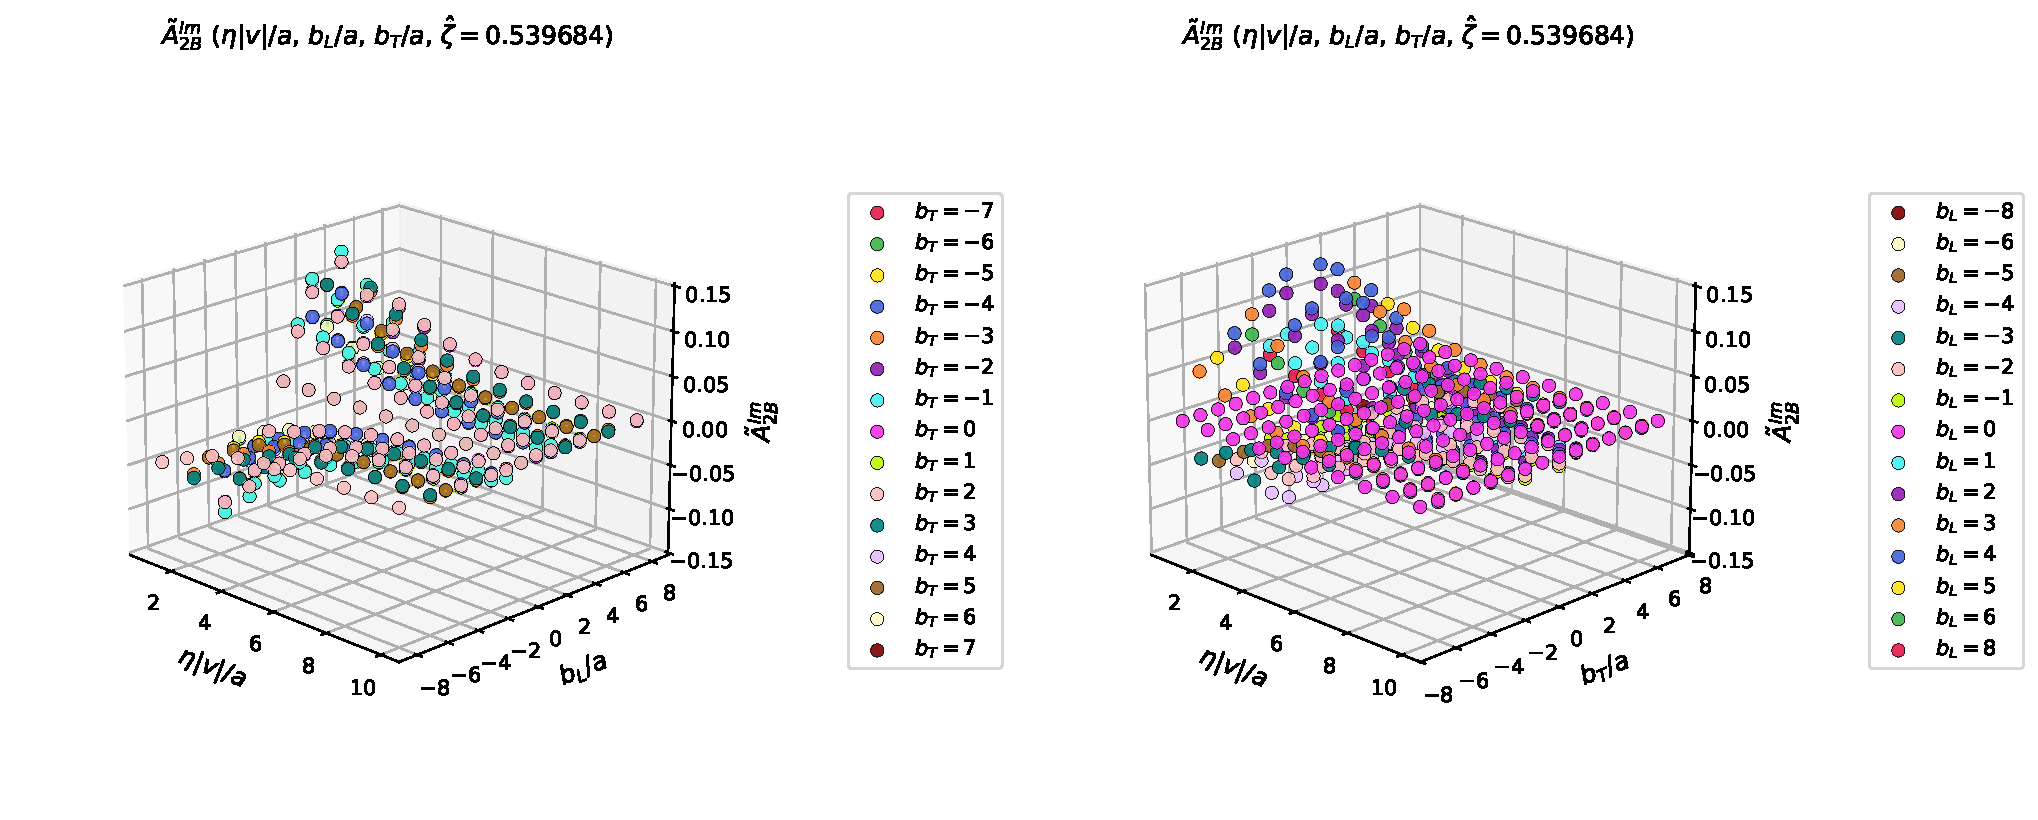
\includegraphics[width=0.7\linewidth]{plots/Amps_bL_bT/ImA2B_PL-3_3D.pdf}
    \caption{Caption}
    \label{fig:placeholder}
\end{figure}
\begin{figure}
    \centering
    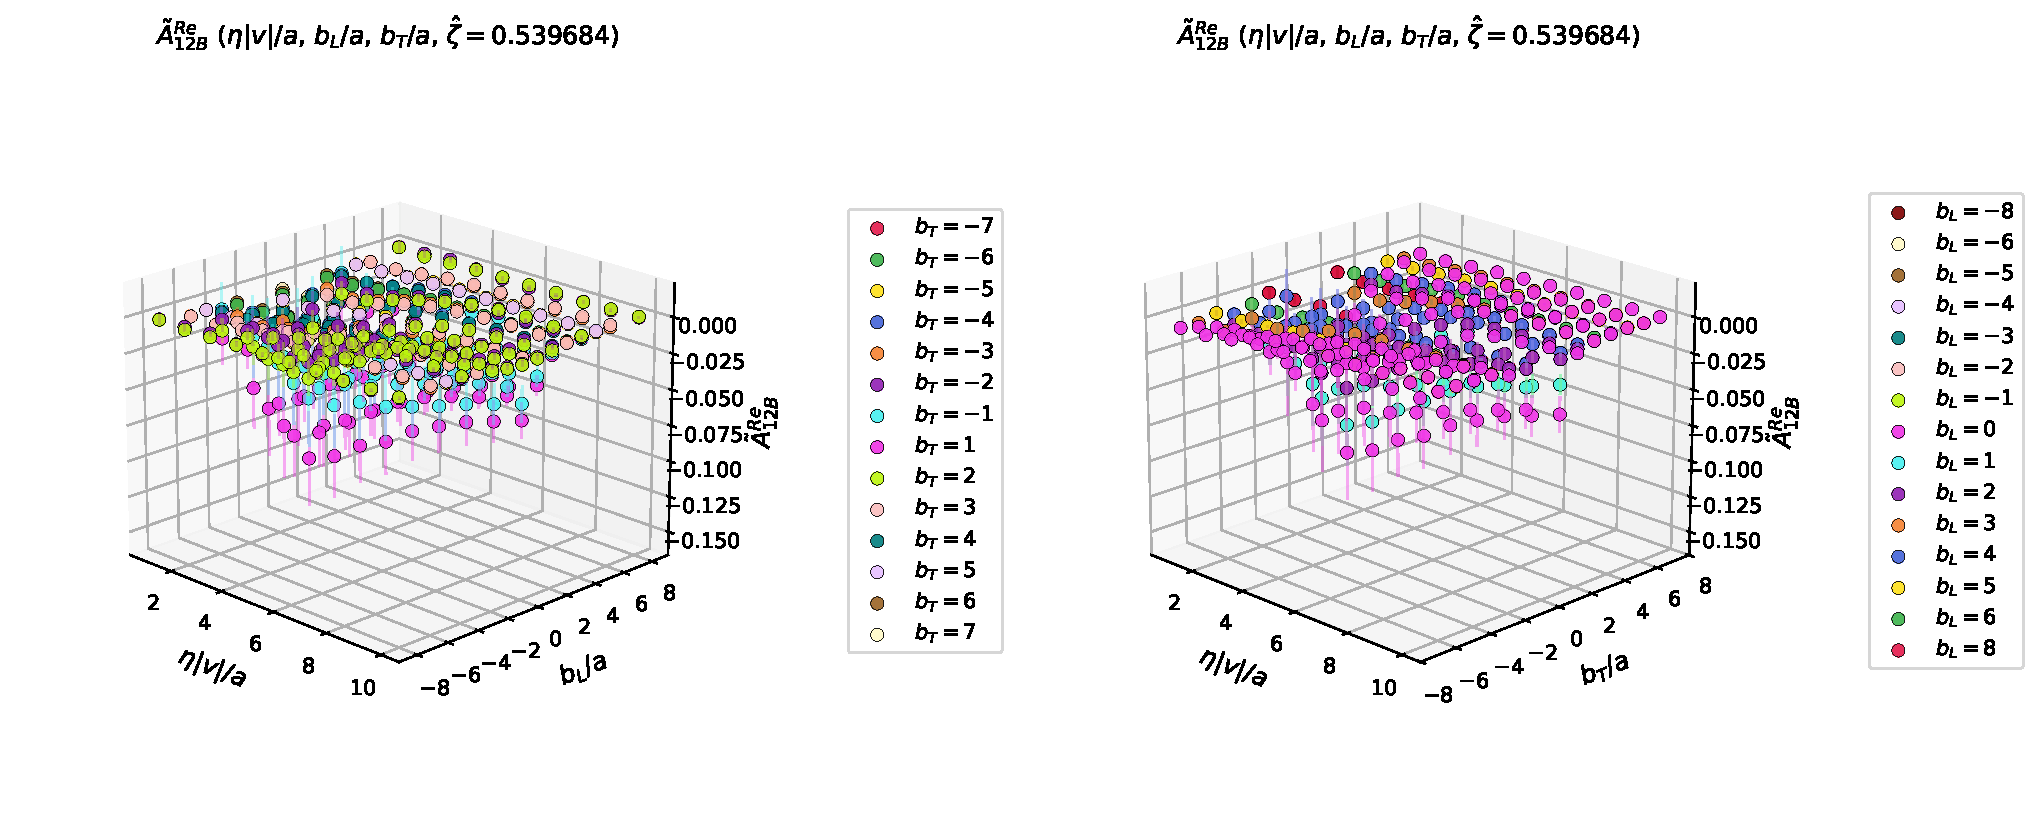
\includegraphics[width=0.7\linewidth]{plots/Amps_bL_bT/ReA12B_PL-3_3D.pdf}
    \caption{Caption}
    \label{fig:placeholder}
\end{figure}
\begin{figure}
    \centering
    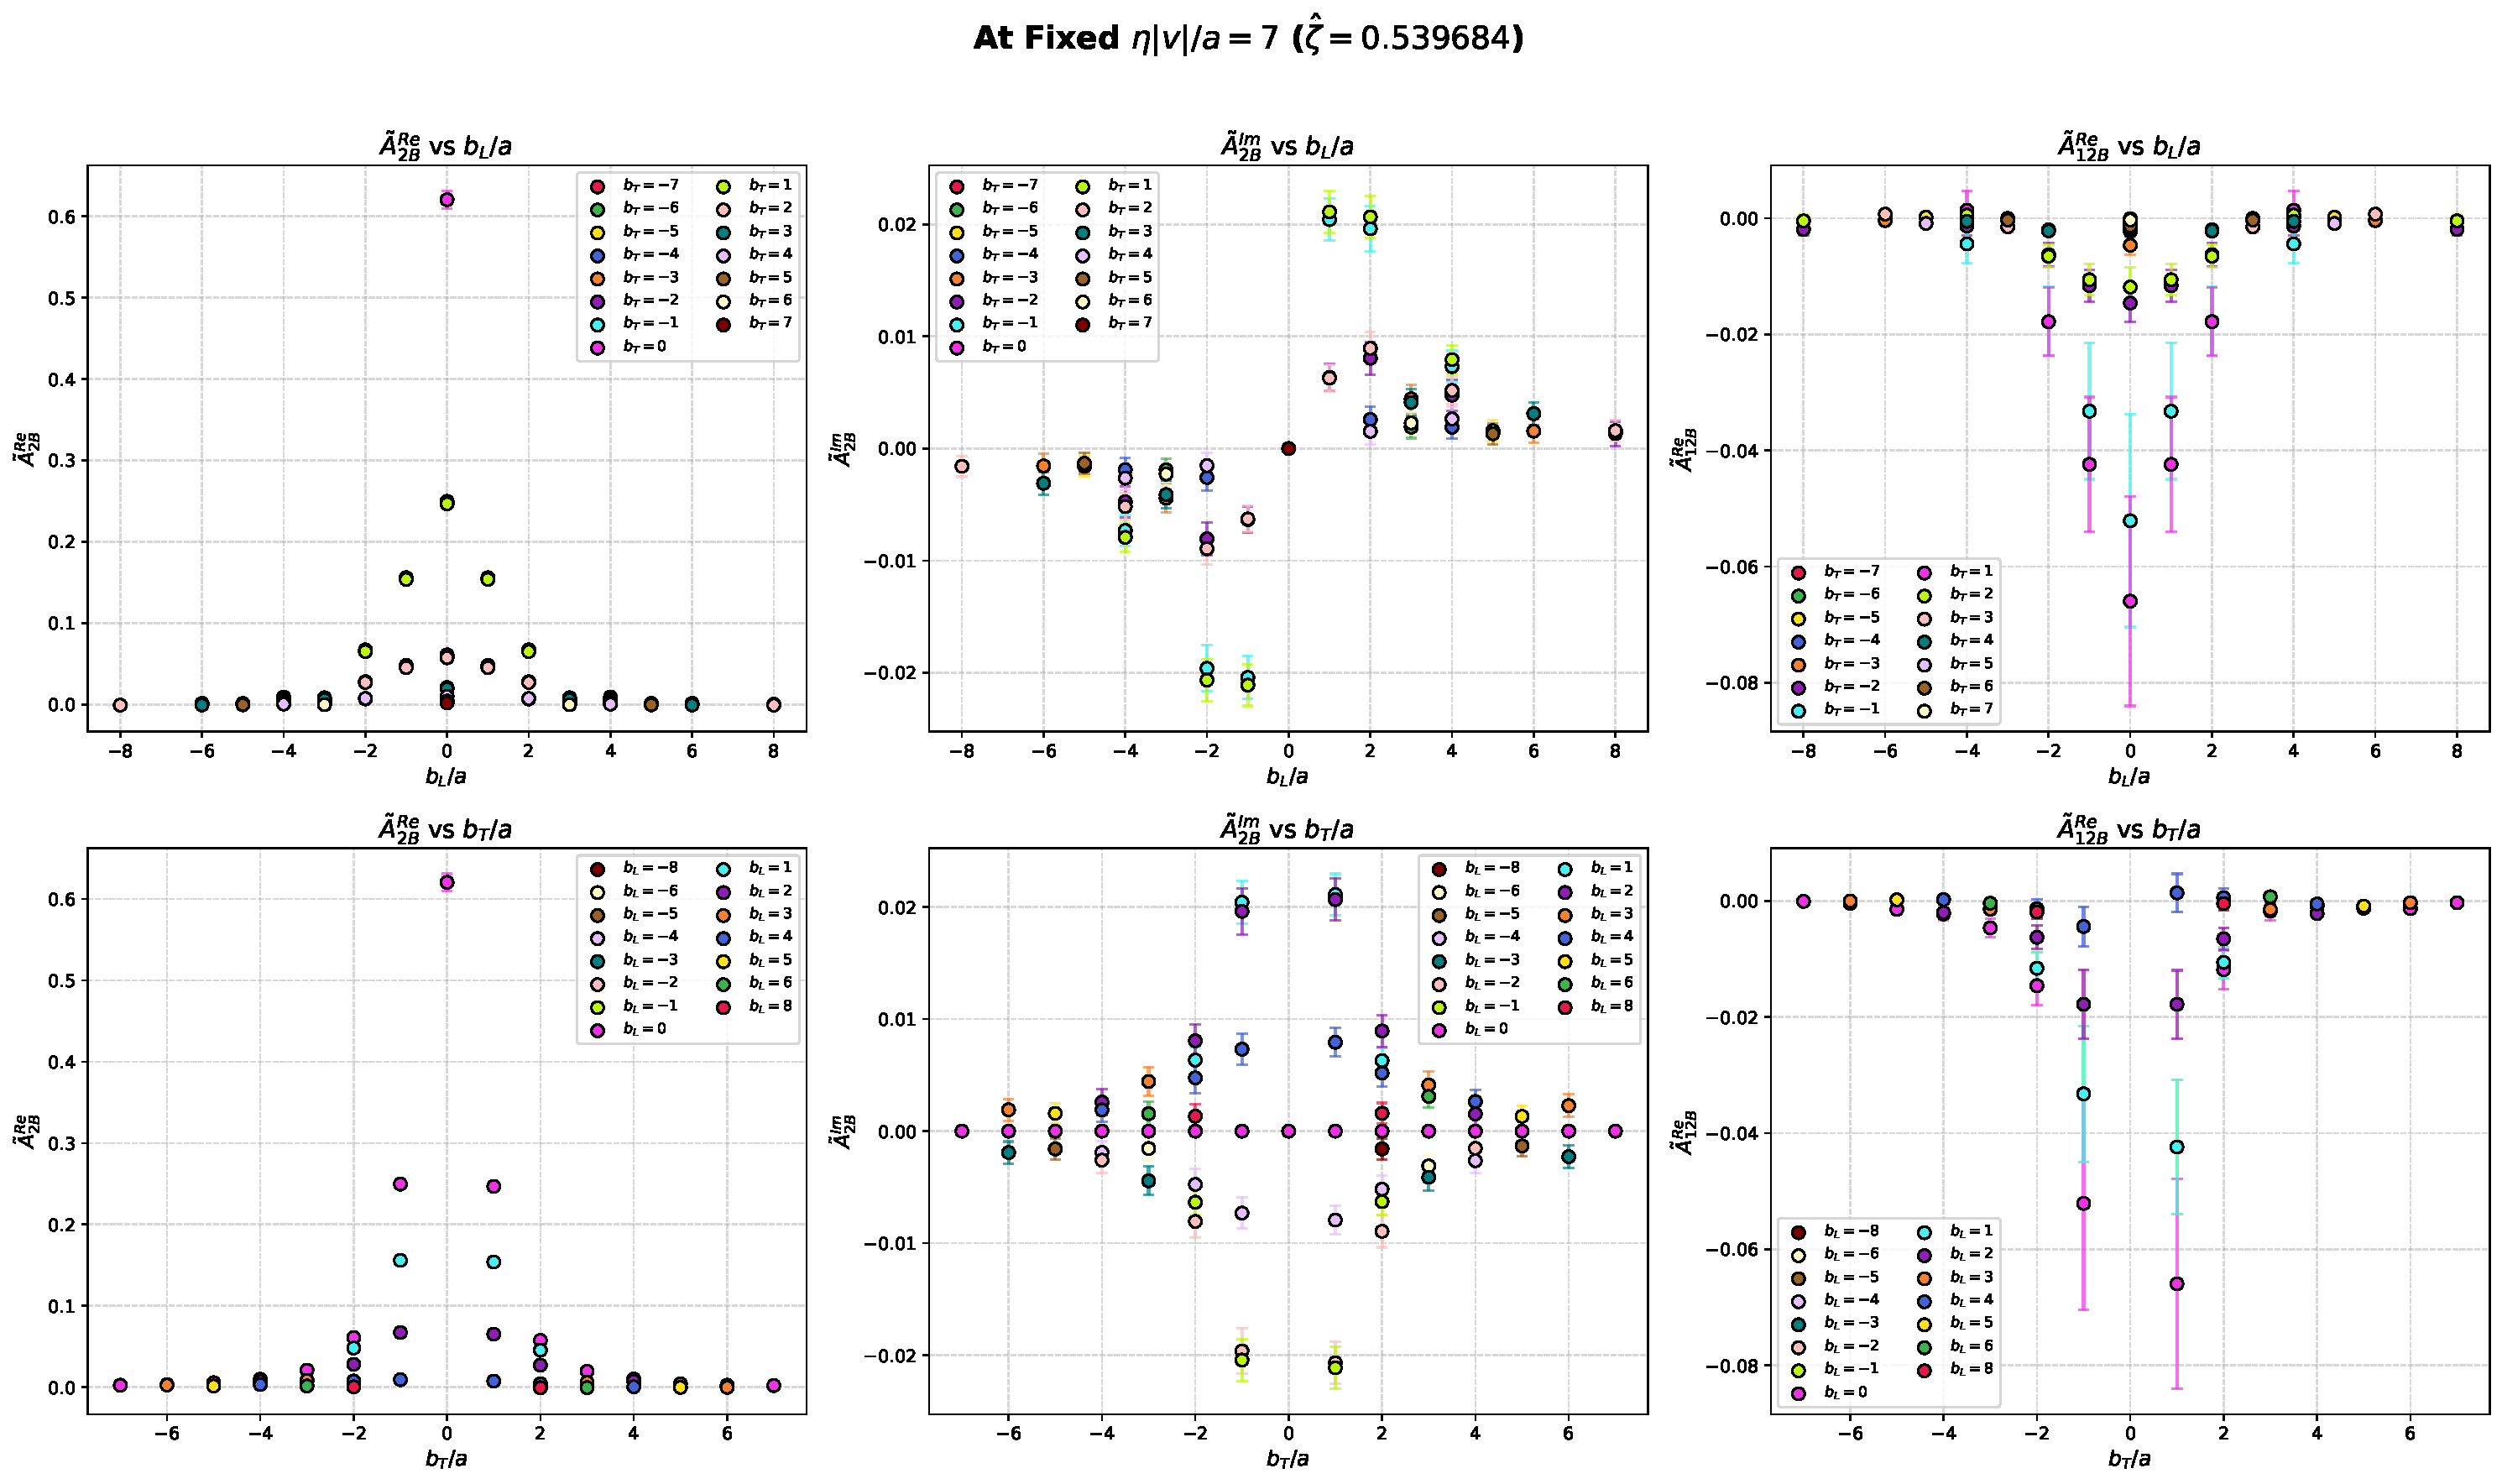
\includegraphics[width=0.7\linewidth]{plots/Amps_bL_bT/Combined_2D_eta7_PL-3.pdf}
    \caption{Caption}
    \label{fig:placeholder}
\end{figure}

\pagebreak
\subsubsection{\texorpdfstring{$\hat{\zeta}=0.785756$}{TEXT}}
\begin{figure}
    \centering
    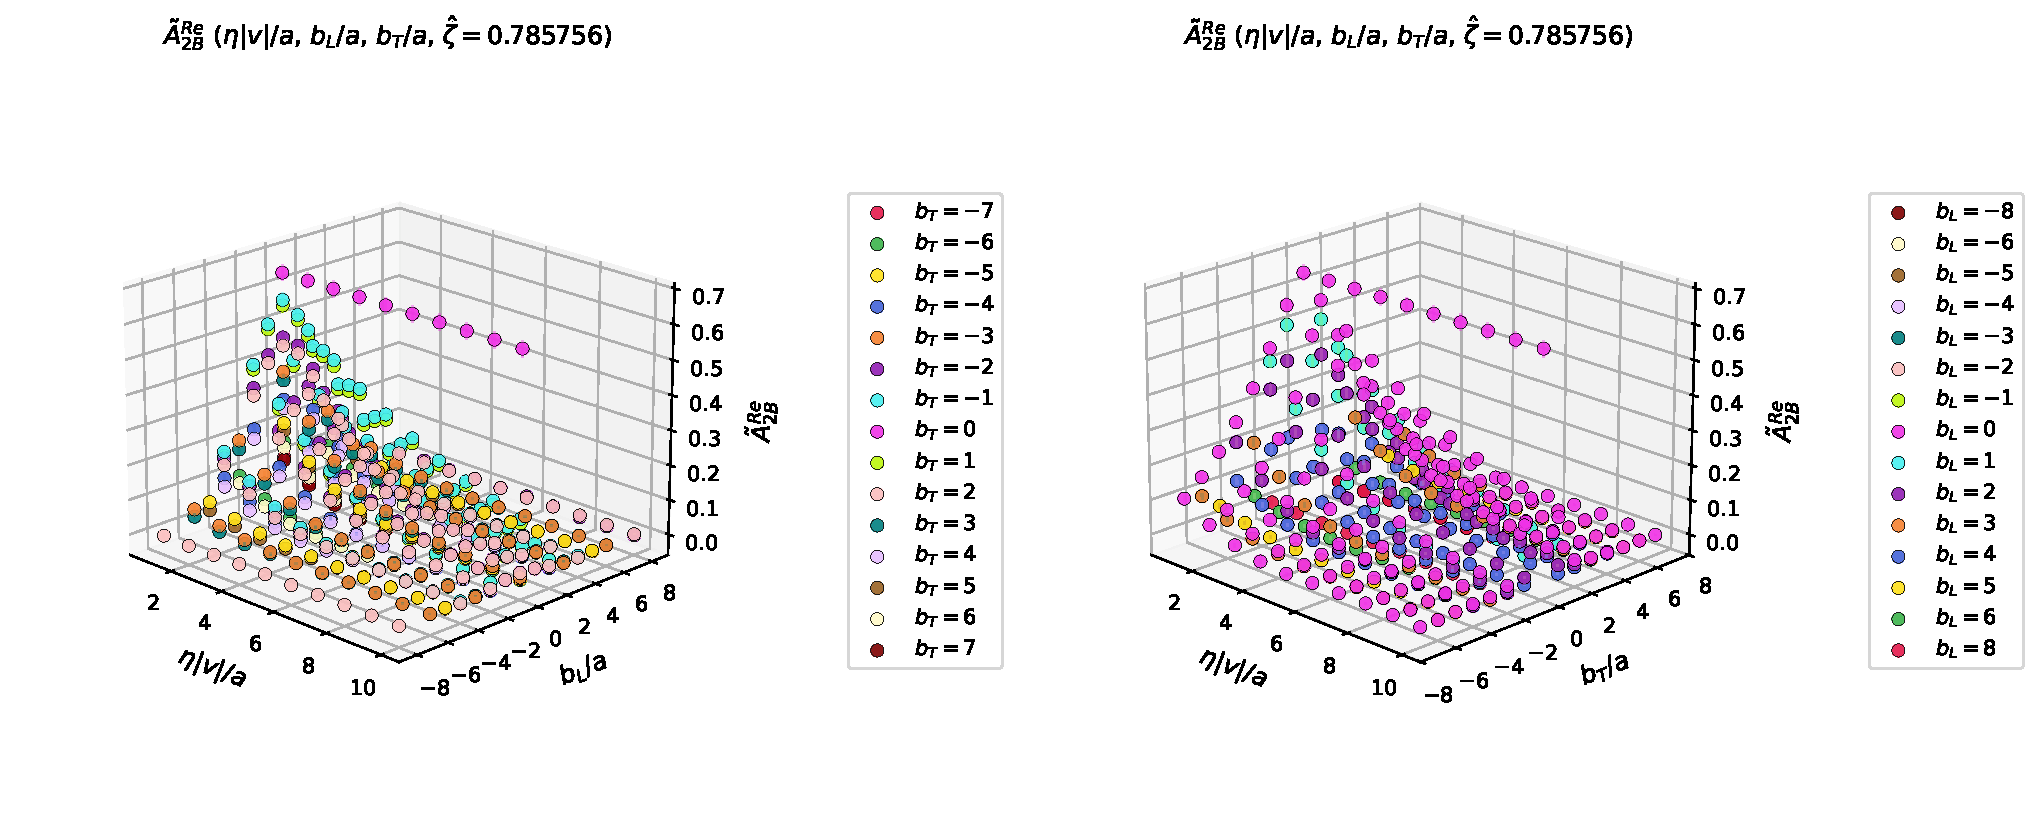
\includegraphics[width=0.7\linewidth]{plots/Amps_bL_bT/ReA2B_PL-4_3D.pdf}
    \caption{Caption}
    \label{fig:placeholder}
\end{figure}
\begin{figure}
    \centering
    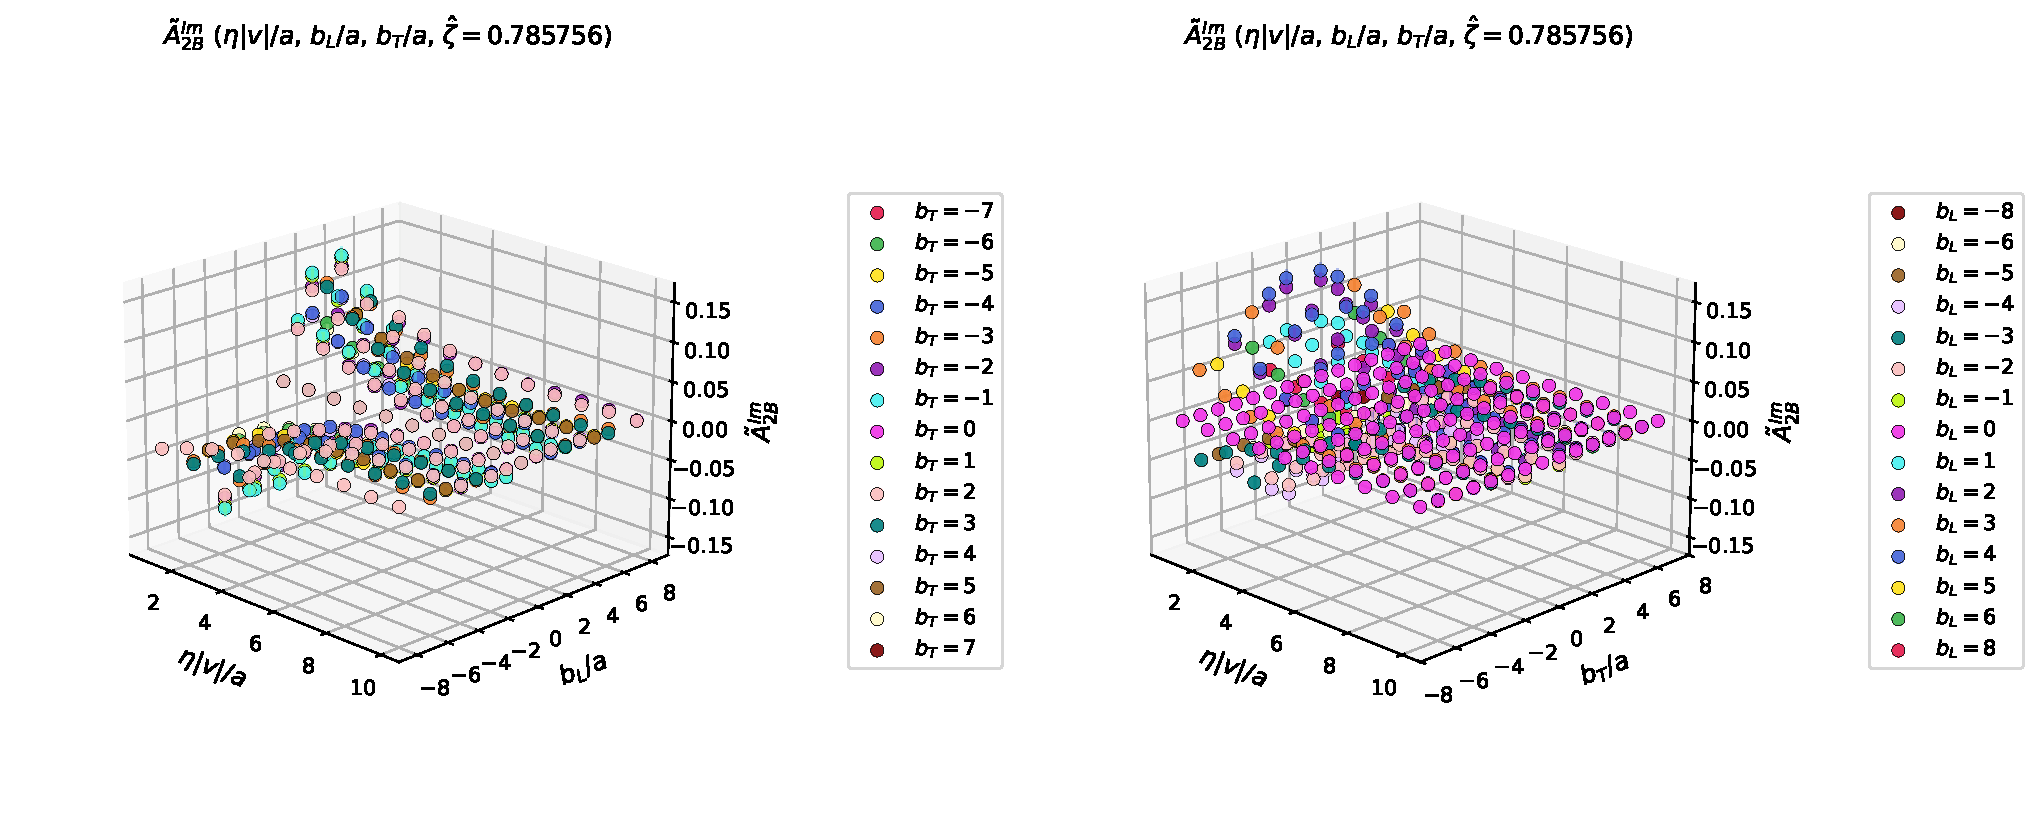
\includegraphics[width=0.7\linewidth]{plots/Amps_bL_bT/ImA2B_PL-4_3D.pdf}
    \caption{Caption}
    \label{fig:placeholder}
\end{figure}
\begin{figure}
    \centering
    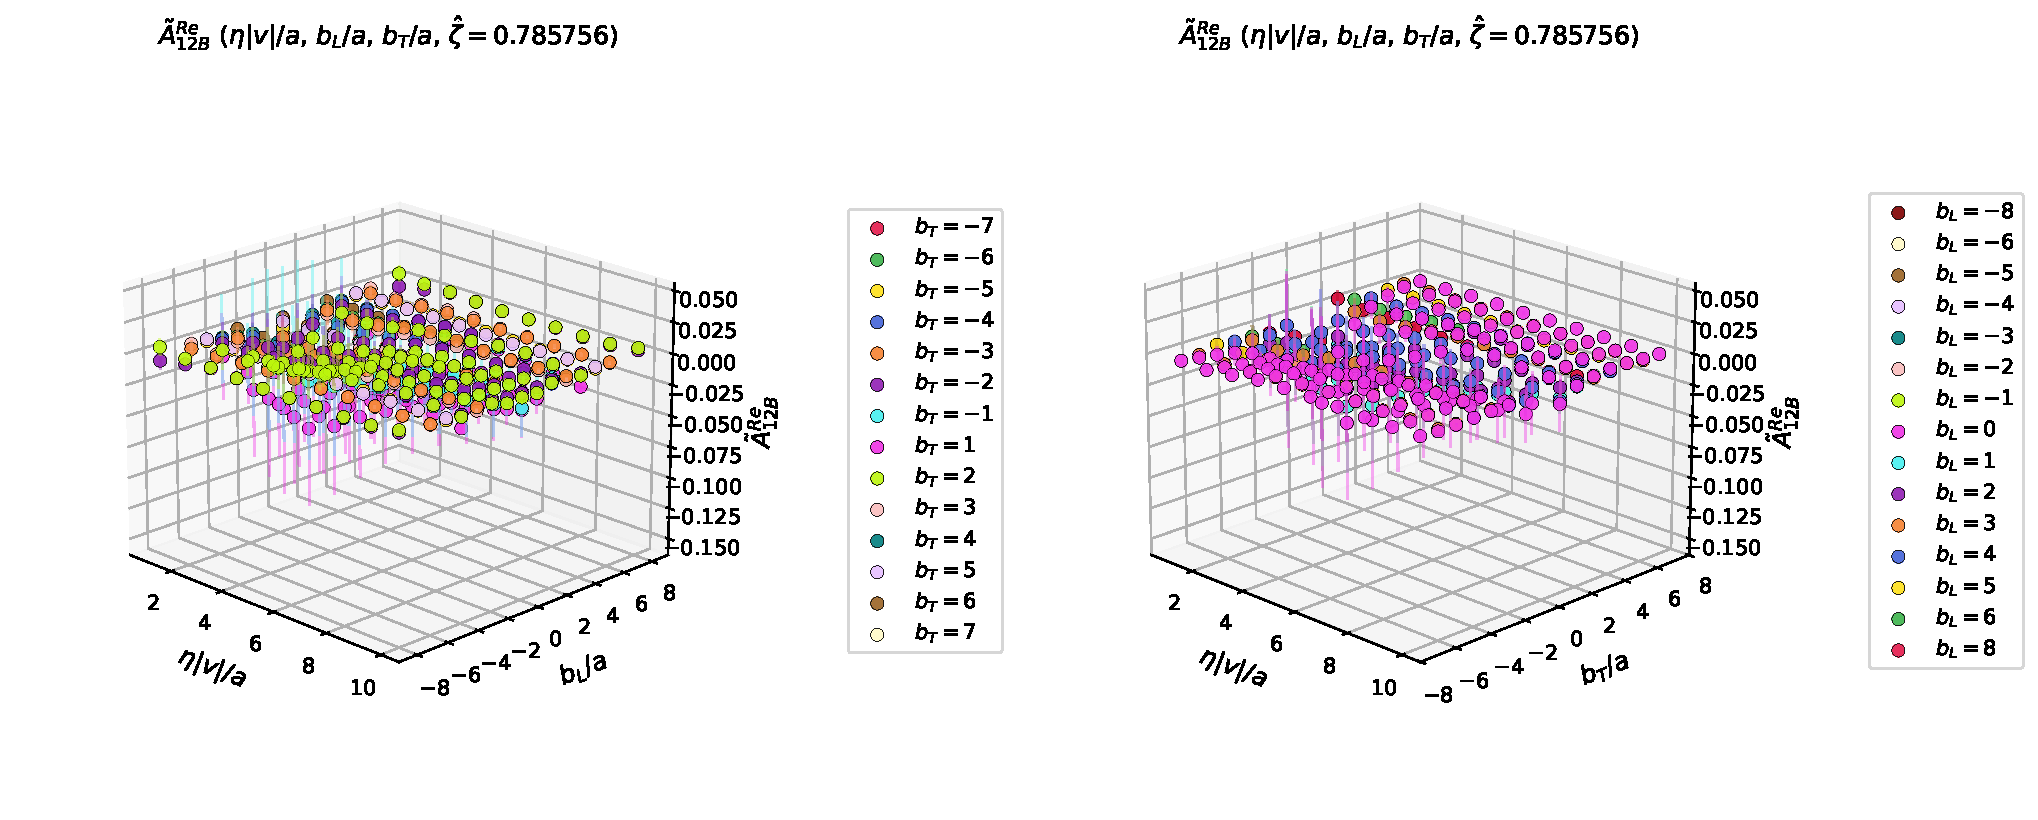
\includegraphics[width=0.7\linewidth]{plots/Amps_bL_bT/ReA12B_PL-4_3D.pdf}
    \caption{Caption}
    \label{fig:placeholder}
\end{figure}
\begin{figure}
    \centering
    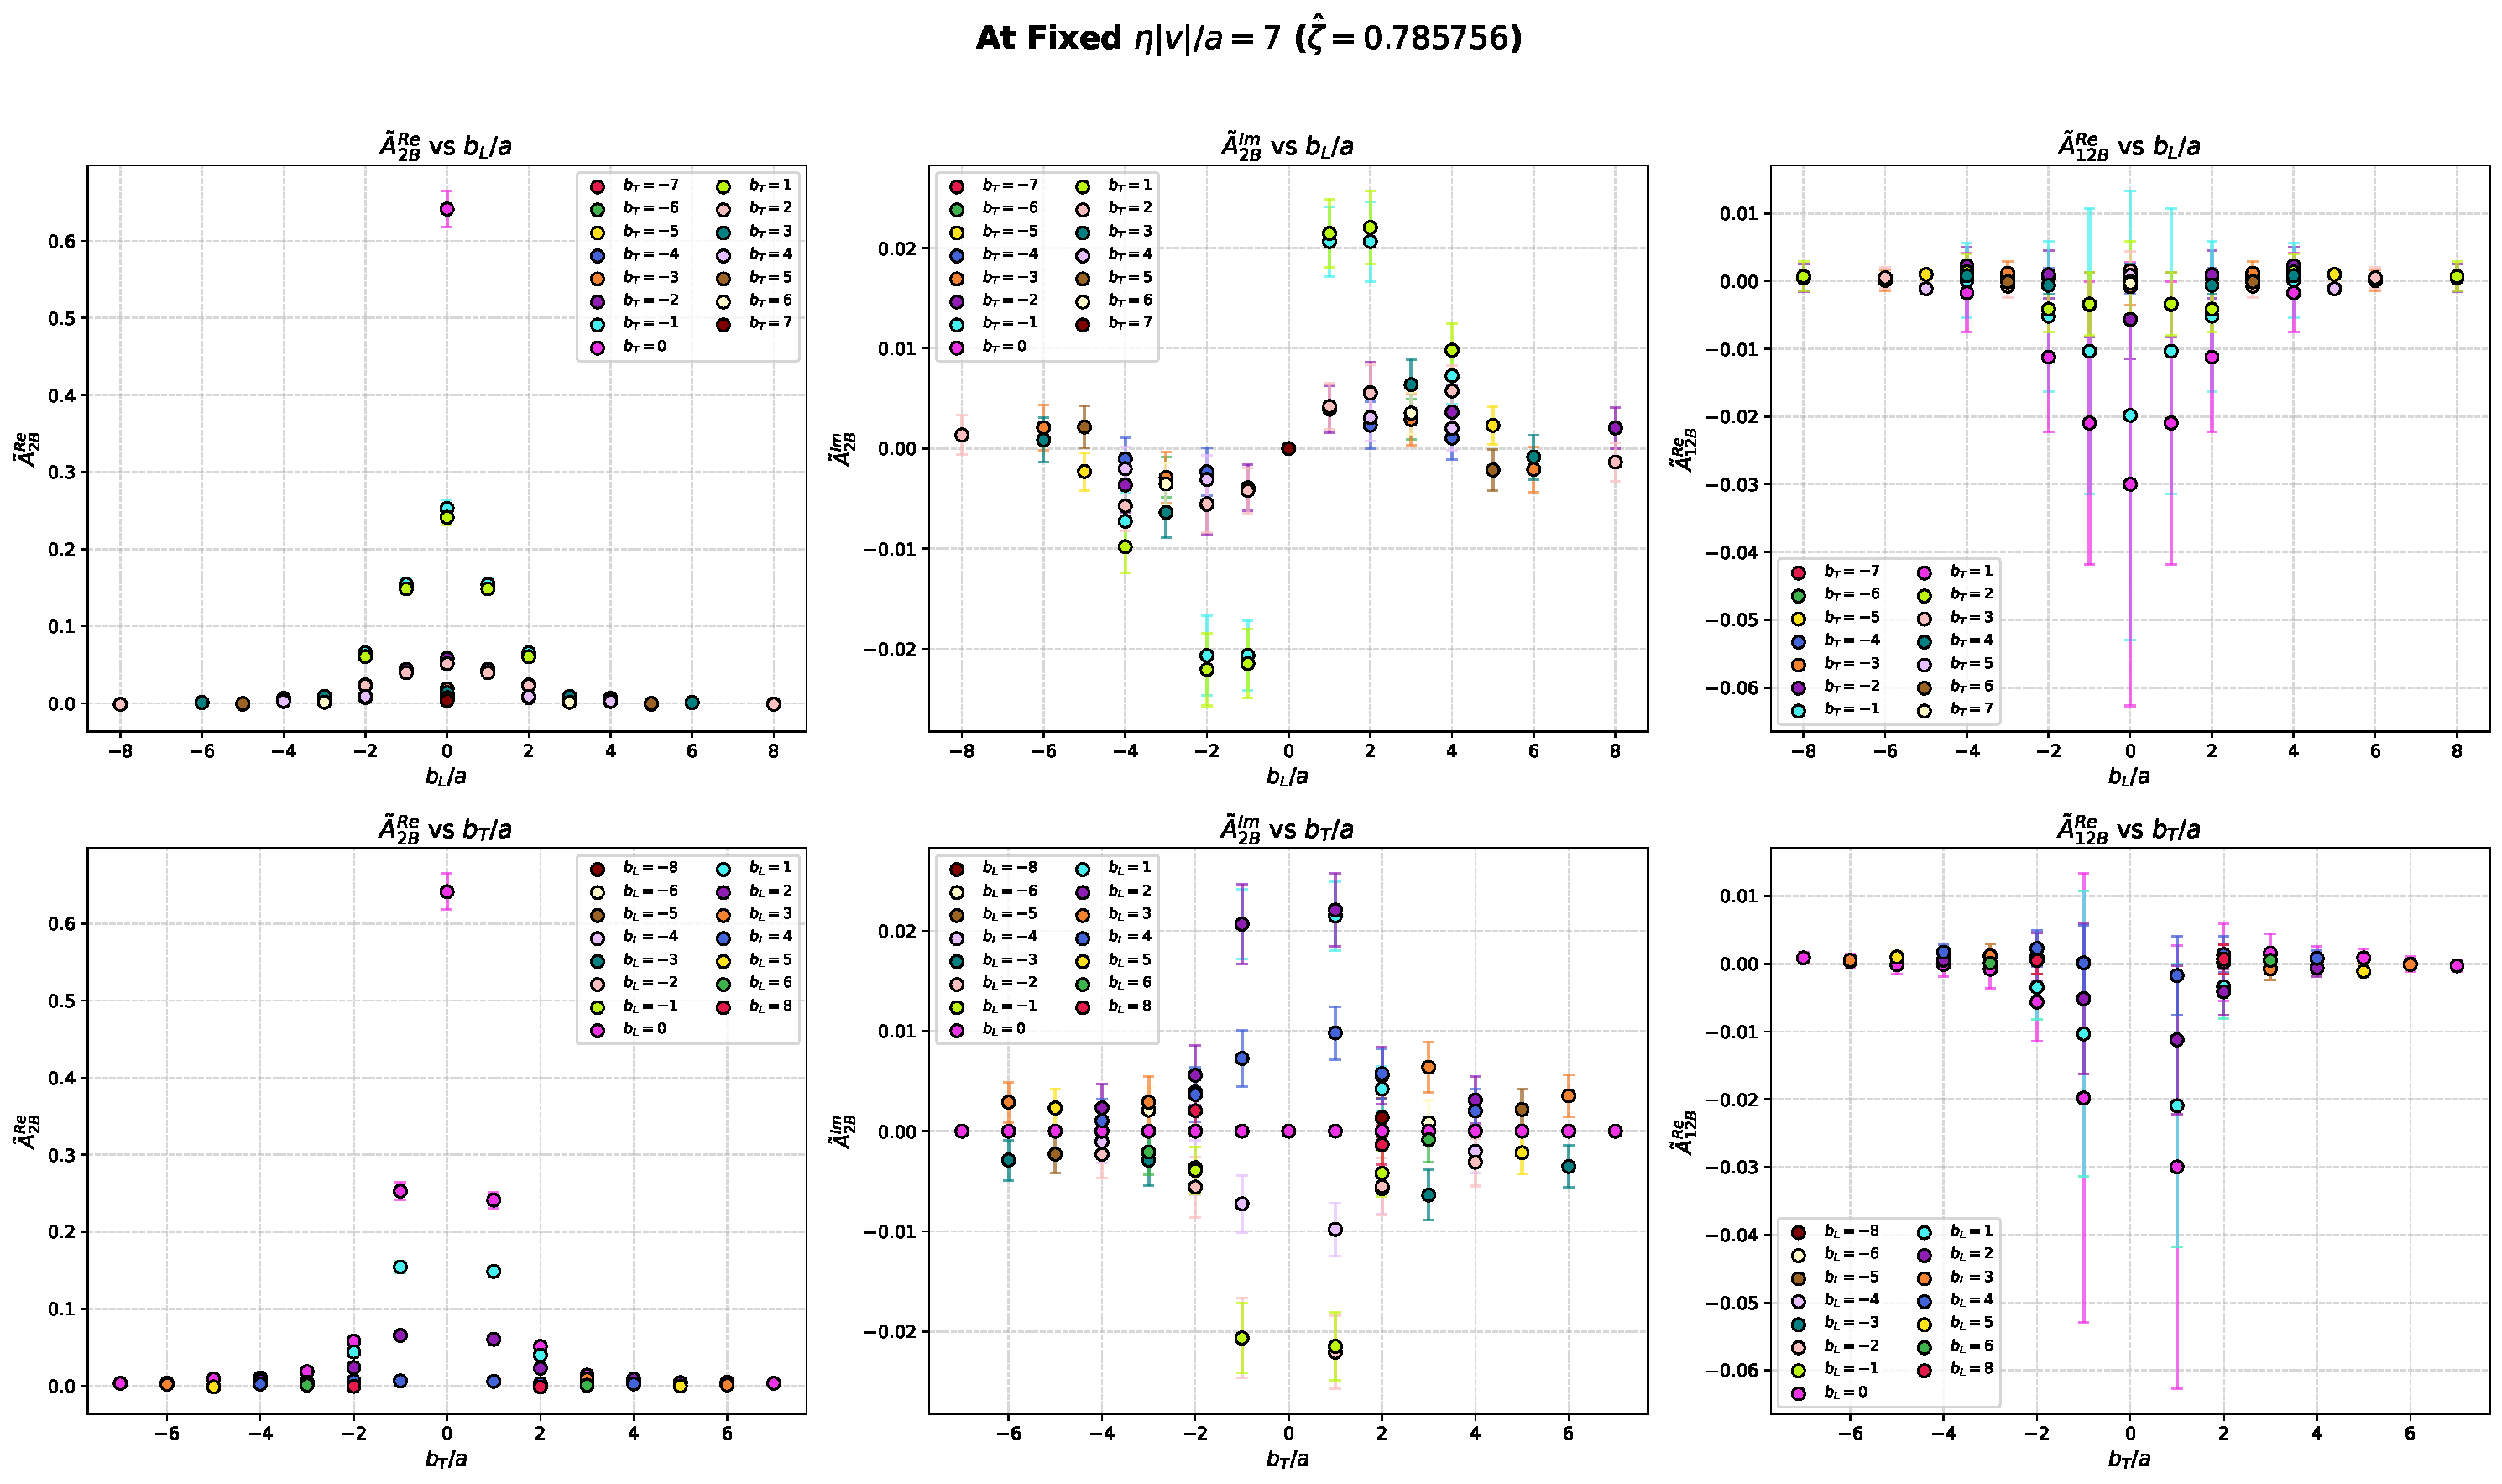
\includegraphics[width=0.7\linewidth]{plots/Amps_bL_bT/Combined_2D_eta7_PL-4.pdf}
    \caption{Caption}
    \label{fig:placeholder}
\end{figure}
